\documentclass[10pt]{article}
\usepackage[margin=2.2cm]{geometry}
\usepackage{booktabs,longtable,graphicx,array}
\usepackage[hidelinks]{hyperref}
\setlength{\tabcolsep}{4pt}
\newcommand{\stackcell}[1]{\begin{tabular}[t]{@{}l@{}}#1\end{tabular}}
\title{tropical: LIS}
\date{2026-10-25T23:07:27}
\begin{document}
\maketitle

\section{Key results}
This report covers 240 runs (5 seeds; 0 diverged) under frozen hash \texttt{69813b292d06}.
\paragraph{Where to look.} The headline metric is \texttt{ood\_len\_f1} (higher is better).
\autoref{fig:ood_len_f1} plots it against \texttt{fishr\_lambda}.
\autoref{tab:summary-ood_len_f1} gives every cell's mean with its 95\% bootstrap CI.
\autoref{tab:control-ood_len_f1} compares each level with the control.
\autoref{tab:trend-ood_len_f1} gives the trend.
\autoref{tab:paired-ood_len_f1} gives the paired contrasts.
Its tests take the parametric path: values away from the metric bounds.
Cells are compared within a seed: a seed index fixes the data and the initialization.
Comparisons are marked significant at $p < 0.05$ after the stated correction.

\subsection{\texttt{ood\_len\_f1}}
\begin{figure}[tbp]
\centering
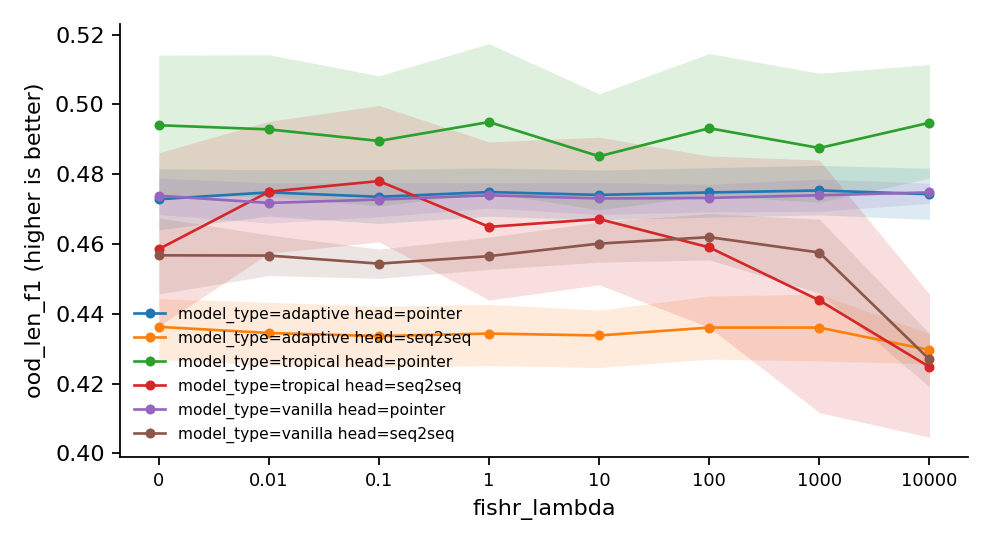
\includegraphics[width=\textwidth]{metric_ood_len_f1.png}
\caption{\texttt{ood\_len\_f1} against \texttt{fishr\_lambda}: the mean over seeds with a 95\% bootstrap CI, one line per combination of the other factors.}
\label{fig:ood_len_f1}
\end{figure}

{\small
\begin{longtable}{lllrlrrr}
\caption{\texttt{ood\_len\_f1} per cell: mean, 95\% bootstrap CI, SD, seeds, diverged runs.}\label{tab:summary-ood_len_f1}\\
\toprule
\texttt{model\_type} & \texttt{head} & \texttt{fishr\_lambda} & mean & 95\% CI & SD & $n$ & div.\\
\midrule
\endhead
adaptive & pointer & 0 & 0.4729 & [0.464, 0.482] & 0.0112 & 5 & 0\\
adaptive & pointer & 0.01 & 0.4748 & [0.468, 0.481] & 0.0086 & 5 & 0\\
adaptive & pointer & 0.1 & 0.4736 & [0.466, 0.481] & 0.00984 & 5 & 0\\
adaptive & pointer & 1 & 0.4749 & [0.468, 0.482] & 0.0088 & 5 & 0\\
adaptive & pointer & 10 & 0.4741 & [0.467, 0.481] & 0.00945 & 5 & 0\\
adaptive & pointer & 100 & 0.4748 & [0.468, 0.482] & 0.00893 & 5 & 0\\
adaptive & pointer & 1000 & 0.4754 & [0.468, 0.483] & 0.00916 & 5 & 0\\
adaptive & pointer & 1e+04 & 0.4743 & [0.467, 0.482] & 0.00988 & 5 & 0\\
adaptive & seq2seq & 0 & 0.4363 & [0.427, 0.444] & 0.0112 & 5 & 0\\
adaptive & seq2seq & 0.01 & 0.4345 & [0.425, 0.443] & 0.0118 & 5 & 0\\
adaptive & seq2seq & 0.1 & 0.4336 & [0.425, 0.442] & 0.0111 & 5 & 0\\
adaptive & seq2seq & 1 & 0.4344 & [0.425, 0.443] & 0.0107 & 5 & 0\\
adaptive & seq2seq & 10 & 0.4338 & [0.425, 0.441] & 0.0105 & 5 & 0\\
adaptive & seq2seq & 100 & 0.4361 & [0.427, 0.445] & 0.0118 & 5 & 0\\
adaptive & seq2seq & 1000 & 0.4361 & [0.427, 0.446] & 0.0123 & 5 & 0\\
adaptive & seq2seq & 1e+04 & 0.4296 & [0.426, 0.434] & 0.00566 & 5 & 0\\
tropical & pointer & 0 & 0.494 & [0.474, 0.514] & 0.0262 & 5 & 0\\
tropical & pointer & 0.01 & 0.4929 & [0.474, 0.514] & 0.0258 & 5 & 0\\
tropical & pointer & 0.1 & 0.4896 & [0.471, 0.508] & 0.0248 & 5 & 0\\
tropical & pointer & 1 & 0.495 & [0.475, 0.517] & 0.03 & 5 & 0\\
tropical & pointer & 10 & 0.4852 & [0.47, 0.503] & 0.0214 & 5 & 0\\
tropical & pointer & 100 & 0.4932 & [0.474, 0.515] & 0.0265 & 5 & 0\\
tropical & pointer & 1000 & 0.4875 & [0.472, 0.509] & 0.0253 & 5 & 0\\
tropical & pointer & 1e+04 & 0.4948 & [0.479, 0.511] & 0.0212 & 5 & 0\\
tropical & seq2seq & 0 & 0.4586 & [0.437, 0.486] & 0.0317 & 5 & 0\\
tropical & seq2seq & 0.01 & 0.475 & [0.457, 0.495] & 0.0265 & 5 & 0\\
tropical & seq2seq & 0.1 & 0.4781 & [0.461, 0.5] & 0.025 & 5 & 0\\
tropical & seq2seq & 1 & 0.4649 & [0.444, 0.489] & 0.0287 & 5 & 0\\
tropical & seq2seq & 10 & 0.4672 & [0.448, 0.491] & 0.028 & 5 & 0\\
tropical & seq2seq & 100 & 0.459 & [0.436, 0.485] & 0.0313 & 5 & 0\\
tropical & seq2seq & 1000 & 0.4439 & [0.412, 0.484] & 0.0475 & 5 & 0\\
tropical & seq2seq & 1e+04 & 0.4248 & [0.405, 0.446] & 0.0251 & 5 & 0\\
vanilla & pointer & 0 & 0.4739 & [0.468, 0.479] & 0.00705 & 5 & 0\\
vanilla & pointer & 0.01 & 0.4718 & [0.466, 0.478] & 0.00761 & 5 & 0\\
vanilla & pointer & 0.1 & 0.4728 & [0.468, 0.478] & 0.00653 & 5 & 0\\
vanilla & pointer & 1 & 0.474 & [0.47, 0.478] & 0.00479 & 5 & 0\\
vanilla & pointer & 10 & 0.4731 & [0.468, 0.478] & 0.00606 & 5 & 0\\
vanilla & pointer & 100 & 0.4732 & [0.469, 0.477] & 0.00525 & 5 & 0\\
vanilla & pointer & 1000 & 0.474 & [0.469, 0.479] & 0.00619 & 5 & 0\\
vanilla & pointer & 1e+04 & 0.4748 & [0.472, 0.477] & 0.00368 & 5 & 0\\
vanilla & seq2seq & 0 & 0.4568 & [0.446, 0.468] & 0.0137 & 5 & 0\\
vanilla & seq2seq & 0.01 & 0.4567 & [0.451, 0.463] & 0.00763 & 5 & 0\\
vanilla & seq2seq & 0.1 & 0.4544 & [0.45, 0.459] & 0.00544 & 5 & 0\\
vanilla & seq2seq & 1 & 0.4565 & [0.453, 0.462] & 0.00596 & 5 & 0\\
vanilla & seq2seq & 10 & 0.4601 & [0.455, 0.466] & 0.0075 & 5 & 0\\
vanilla & seq2seq & 100 & 0.462 & [0.455, 0.469] & 0.00874 & 5 & 0\\
vanilla & seq2seq & 1000 & 0.4576 & [0.446, 0.467] & 0.0139 & 5 & 0\\
vanilla & seq2seq & 1e+04 & 0.4269 & [0.419, 0.434] & 0.00985 & 5 & 0\\
\bottomrule
\end{longtable}
}

{\small
\begin{longtable}{lllrrrl}
\caption{\texttt{ood\_len\_f1}: each level of \texttt{fishr\_lambda} against its control (0), within each combination of the other factors. parametric: Dunnett vs control.}\label{tab:control-ood_len_f1}\\
\toprule
\texttt{model\_type} & \texttt{head} & \texttt{fishr\_lambda} & difference & 95\% CI & $p$ & \\
\midrule
\endhead
adaptive & pointer & 0.01 & 0.001966 & [-0.0147, 0.0186] & 0.9997 & \\
adaptive & pointer & 0.1 & $7.002\times10^{-4}$ & [-0.0159, 0.0173] & 1.0000 & \\
adaptive & pointer & 1 & 0.00205 & [-0.0146, 0.0187] & 0.9996 & \\
adaptive & pointer & 10 & 0.001234 & [-0.0154, 0.0179] & 1.0000 & \\
adaptive & pointer & 100 & 0.001936 & [-0.0147, 0.0186] & 0.9997 & \\
adaptive & pointer & 1000 & 0.00251 & [-0.0141, 0.0191] & 0.9985 & \\
adaptive & pointer & 1e+04 & 0.001455 & [-0.0152, 0.0181] & 1.0000 & \\
adaptive & seq2seq & 0.01 & -0.001755 & [-0.0206, 0.0171] & 0.9999 & \\
adaptive & seq2seq & 0.1 & -0.002651 & [-0.0215, 0.0162] & 0.9990 & \\
adaptive & seq2seq & 1 & -0.001922 & [-0.0208, 0.017] & 0.9999 & \\
adaptive & seq2seq & 10 & -0.00247 & [-0.0213, 0.0164] & 0.9994 & \\
adaptive & seq2seq & 100 & $-1.977\times10^{-4}$ & [-0.0191, 0.0187] & 1.0000 & \\
adaptive & seq2seq & 1000 & $-2.062\times10^{-4}$ & [-0.0191, 0.0187] & 1.0000 & \\
adaptive & seq2seq & 1e+04 & -0.006635 & [-0.0255, 0.0122] & 0.8702 & \\
tropical & pointer & 0.01 & -0.001179 & [-0.0454, 0.043] & 1.0000 & \\
tropical & pointer & 0.1 & -0.004494 & [-0.0487, 0.0397] & 0.9999 & \\
tropical & pointer & 1 & $9.210\times10^{-4}$ & [-0.0433, 0.0451] & 1.0000 & \\
tropical & pointer & 10 & -0.008895 & [-0.0531, 0.0353] & 0.9914 & \\
tropical & pointer & 100 & $-8.480\times10^{-4}$ & [-0.045, 0.0433] & 1.0000 & \\
tropical & pointer & 1000 & -0.006517 & [-0.0507, 0.0377] & 0.9987 & \\
tropical & pointer & 1e+04 & $7.178\times10^{-4}$ & [-0.0435, 0.0449] & 1.0000 & \\
tropical & seq2seq & 0.01 & 0.01644 & [-0.0381, 0.071] & 0.9321 & \\
tropical & seq2seq & 0.1 & 0.0195 & [-0.0351, 0.0741] & 0.8617 & \\
tropical & seq2seq & 1 & 0.006372 & [-0.0482, 0.0609] & 0.9997 & \\
tropical & seq2seq & 10 & 0.008602 & [-0.046, 0.0632] & 0.9980 & \\
tropical & seq2seq & 100 & $4.860\times10^{-4}$ & [-0.0541, 0.0551] & 1.0000 & \\
tropical & seq2seq & 1000 & -0.01468 & [-0.0693, 0.0399] & 0.9600 & \\
tropical & seq2seq & 1e+04 & -0.03377 & [-0.0883, 0.0208] & 0.3845 & \\
vanilla & pointer & 0.01 & -0.002072 & [-0.0126, 0.00843] & 0.9924 & \\
vanilla & pointer & 0.1 & -0.001092 & [-0.0116, 0.00941] & 0.9999 & \\
vanilla & pointer & 1 & $1.152\times10^{-4}$ & [-0.0104, 0.0106] & 1.0000 & \\
vanilla & pointer & 10 & $-7.854\times10^{-4}$ & [-0.0113, 0.00972] & 1.0000 & \\
vanilla & pointer & 100 & $-6.320\times10^{-4}$ & [-0.0111, 0.00987] & 1.0000 & \\
vanilla & pointer & 1000 & $1.260\times10^{-4}$ & [-0.0104, 0.0106] & 1.0000 & \\
vanilla & pointer & 1e+04 & $9.510\times10^{-4}$ & [-0.00955, 0.0115] & 0.9999 & \\
vanilla & seq2seq & 0.01 & $-6.422\times10^{-5}$ & [-0.0168, 0.0167] & 1.0000 & \\
vanilla & seq2seq & 0.1 & -0.002382 & [-0.0191, 0.0144] & 0.9989 & \\
vanilla & seq2seq & 1 & $-2.292\times10^{-4}$ & [-0.017, 0.0165] & 1.0000 & \\
vanilla & seq2seq & 10 & 0.00336 & [-0.0134, 0.0201] & 0.9916 & \\
vanilla & seq2seq & 100 & 0.005209 & [-0.0115, 0.0219] & 0.9215 & \\
vanilla & seq2seq & 1000 & $7.980\times10^{-4}$ & [-0.0159, 0.0175] & 1.0000 & \\
vanilla & seq2seq & 1e+04 & -0.02983 & [-0.0466, -0.0131] & 0.0002 & *\\
\bottomrule
\end{longtable}
}

{\small
\begin{longtable}{llrrrrr}
\caption{\texttt{ood\_len\_f1} against log10 \texttt{fishr\_lambda}: parametric: OLS slope t-test, seed-bootstrap CI, with the Jonckheere--Terpstra ordered-trend $\tau$ and $p$.}\label{tab:trend-ood_len_f1}\\
\toprule
\texttt{model\_type} & \texttt{head} & estimate & 95\% CI & $p$ & JT $\tau$ & JT $p$\\
\midrule
\endhead
adaptive & pointer & $7.052\times10^{-5}$ & [$-1.45\times10^{-4}$, $2.69\times10^{-4}$] & 0.9227 & 0.0514 & 0.7031\\
adaptive & seq2seq & $-2.867\times10^{-4}$ & [-0.00158, $9.51\times10^{-4}$] & 0.7392 & -0.0362 & 0.8090\\
tropical & pointer & $-4.458\times10^{-6}$ & [-0.00113, 0.00123] & 0.9982 & 0.0133 & 0.9312\\
tropical & seq2seq & -0.008031 & [-0.0106, -0.00582] & 0.0029 & -0.406 & 0.0020\\
vanilla & pointer & $3.842\times10^{-4}$ & [$-5.00\times10^{-5}$, $8.47\times10^{-4}$] & 0.4071 & 0.0781 & 0.5735\\
vanilla & seq2seq & -0.002768 & [-0.00451, -0.00103] & 0.0152 & -0.101 & 0.4489\\
\bottomrule
\end{longtable}
}

{\small
\begin{longtable}{lrrrl}
\caption{\texttt{ood\_len\_f1}: paired contrasts by seed, Holm-corrected across the cells. parametric: paired t-test by seed, Holm.}\label{tab:paired-ood_len_f1}\\
\toprule
contrast (within) & difference & 95\% CI & $p$ & \\
\midrule
\endhead
\stackcell{model\_type: tropical - vanilla\\\footnotesize head=pointer fishr\_lambda=0 } & 0.02019 & [-0.0132, 0.0536] & 1.0000 & \\
\stackcell{model\_type: tropical - vanilla\\\footnotesize head=pointer fishr\_lambda=0.01 } & 0.02108 & [-0.0152, 0.0574] & 1.0000 & \\
\stackcell{model\_type: tropical - vanilla\\\footnotesize head=pointer fishr\_lambda=0.1 } & 0.01679 & [-0.0173, 0.0508] & 1.0000 & \\
\stackcell{model\_type: tropical - vanilla\\\footnotesize head=pointer fishr\_lambda=1 } & 0.021 & [-0.0183, 0.0603] & 1.0000 & \\
\stackcell{model\_type: tropical - vanilla\\\footnotesize head=pointer fishr\_lambda=10 } & 0.01208 & [-0.016, 0.0402] & 1.0000 & \\
\stackcell{model\_type: tropical - vanilla\\\footnotesize head=pointer fishr\_lambda=100 } & 0.01998 & [-0.0146, 0.0545] & 1.0000 & \\
\stackcell{model\_type: tropical - vanilla\\\footnotesize head=pointer fishr\_lambda=1000 } & 0.01355 & [-0.0237, 0.0508] & 1.0000 & \\
\stackcell{model\_type: tropical - vanilla\\\footnotesize head=pointer fishr\_lambda=1e+04 } & 0.01996 & [-0.0094, 0.0493] & 1.0000 & \\
\stackcell{model\_type: tropical - vanilla\\\footnotesize head=seq2seq fishr\_lambda=0 } & 0.001784 & [-0.0369, 0.0405] & 1.0000 & \\
\stackcell{model\_type: tropical - vanilla\\\footnotesize head=seq2seq fishr\_lambda=0.01 } & 0.01829 & [-0.0162, 0.0527] & 1.0000 & \\
\stackcell{model\_type: tropical - vanilla\\\footnotesize head=seq2seq fishr\_lambda=0.1 } & 0.02366 & [-0.0108, 0.0581] & 1.0000 & \\
\stackcell{model\_type: tropical - vanilla\\\footnotesize head=seq2seq fishr\_lambda=1 } & 0.008385 & [-0.0332, 0.0499] & 1.0000 & \\
\stackcell{model\_type: tropical - vanilla\\\footnotesize head=seq2seq fishr\_lambda=10 } & 0.007026 & [-0.0328, 0.0469] & 1.0000 & \\
\stackcell{model\_type: tropical - vanilla\\\footnotesize head=seq2seq fishr\_lambda=100 } & -0.002939 & [-0.0383, 0.0324] & 1.0000 & \\
\stackcell{model\_type: tropical - vanilla\\\footnotesize head=seq2seq fishr\_lambda=1000 } & -0.0137 & [-0.0678, 0.0404] & 1.0000 & \\
\stackcell{model\_type: tropical - vanilla\\\footnotesize head=seq2seq fishr\_lambda=1e+04 } & -0.002155 & [-0.0247, 0.0204] & 1.0000 & \\
\stackcell{model\_type: adaptive - vanilla\\\footnotesize head=pointer fishr\_lambda=0 } & -0.001006 & [-0.0199, 0.0178] & 1.0000 & \\
\stackcell{model\_type: adaptive - vanilla\\\footnotesize head=pointer fishr\_lambda=0.01 } & 0.003031 & [-0.014, 0.02] & 1.0000 & \\
\stackcell{model\_type: adaptive - vanilla\\\footnotesize head=pointer fishr\_lambda=0.1 } & $7.865\times10^{-4}$ & [-0.0166, 0.0182] & 1.0000 & \\
\stackcell{model\_type: adaptive - vanilla\\\footnotesize head=pointer fishr\_lambda=1 } & $9.283\times10^{-4}$ & [-0.0138, 0.0157] & 1.0000 & \\
\stackcell{model\_type: adaptive - vanilla\\\footnotesize head=pointer fishr\_lambda=10 } & 0.001014 & [-0.0157, 0.0178] & 1.0000 & \\
\stackcell{model\_type: adaptive - vanilla\\\footnotesize head=pointer fishr\_lambda=100 } & 0.001562 & [-0.0138, 0.0169] & 1.0000 & \\
\stackcell{model\_type: adaptive - vanilla\\\footnotesize head=pointer fishr\_lambda=1000 } & 0.001378 & [-0.0154, 0.0181] & 1.0000 & \\
\stackcell{model\_type: adaptive - vanilla\\\footnotesize head=pointer fishr\_lambda=1e+04 } & $-5.025\times10^{-4}$ & [-0.0163, 0.0152] & 1.0000 & \\
\stackcell{model\_type: adaptive - vanilla\\\footnotesize head=seq2seq fishr\_lambda=0 } & -0.0205 & [-0.0481, 0.00709] & 1.0000 & \\
\stackcell{model\_type: adaptive - vanilla\\\footnotesize head=seq2seq fishr\_lambda=0.01 } & -0.02219 & [-0.0421, -0.00232] & 0.5068 & \\
\stackcell{model\_type: adaptive - vanilla\\\footnotesize head=seq2seq fishr\_lambda=0.1 } & -0.02077 & [-0.0396, -0.00194] & 0.5068 & \\
\stackcell{model\_type: adaptive - vanilla\\\footnotesize head=seq2seq fishr\_lambda=1 } & -0.02219 & [-0.0387, -0.00569] & 0.3031 & \\
\stackcell{model\_type: adaptive - vanilla\\\footnotesize head=seq2seq fishr\_lambda=10 } & -0.02633 & [-0.0442, -0.00845] & 0.2397 & \\
\stackcell{model\_type: adaptive - vanilla\\\footnotesize head=seq2seq fishr\_lambda=100 } & -0.0259 & [-0.0503, -0.00147] & 0.5071 & \\
\stackcell{model\_type: adaptive - vanilla\\\footnotesize head=seq2seq fishr\_lambda=1000 } & -0.0215 & [-0.0474, 0.0044] & 0.9075 & \\
\stackcell{model\_type: adaptive - vanilla\\\footnotesize head=seq2seq fishr\_lambda=1e+04 } & 0.002698 & [-0.0145, 0.0198] & 1.0000 & \\
\stackcell{head: pointer - seq2seq\\\footnotesize model\_type=adaptive fishr\_lambda=0 } & 0.03657 & [0.0116, 0.0615] & 0.1984 & \\
\stackcell{head: pointer - seq2seq\\\footnotesize model\_type=adaptive fishr\_lambda=0.01 } & 0.04029 & [0.0201, 0.0605] & 0.0987 & \\
\stackcell{head: pointer - seq2seq\\\footnotesize model\_type=adaptive fishr\_lambda=0.1 } & 0.03992 & [0.0198, 0.06] & 0.0987 & \\
\stackcell{head: pointer - seq2seq\\\footnotesize model\_type=adaptive fishr\_lambda=1 } & 0.04054 & [0.0216, 0.0595] & 0.0806 & \\
\stackcell{head: pointer - seq2seq\\\footnotesize model\_type=adaptive fishr\_lambda=10 } & 0.04028 & [0.0189, 0.0616] & 0.1076 & \\
\stackcell{head: pointer - seq2seq\\\footnotesize model\_type=adaptive fishr\_lambda=100 } & 0.03871 & [0.0162, 0.0612] & 0.1417 & \\
\stackcell{head: pointer - seq2seq\\\footnotesize model\_type=adaptive fishr\_lambda=1000 } & 0.03929 & [0.0151, 0.0634] & 0.1603 & \\
\stackcell{head: pointer - seq2seq\\\footnotesize model\_type=adaptive fishr\_lambda=1e+04 } & 0.04466 & [0.0293, 0.0601] & 0.0297 & *\\
\stackcell{head: pointer - seq2seq\\\footnotesize model\_type=tropical fishr\_lambda=0 } & 0.03549 & [0.00817, 0.0628] & 0.2716 & \\
\stackcell{head: pointer - seq2seq\\\footnotesize model\_type=tropical fishr\_lambda=0.01 } & 0.01787 & [-0.0233, 0.0591] & 0.7449 & \\
\stackcell{head: pointer - seq2seq\\\footnotesize model\_type=tropical fishr\_lambda=0.1 } & 0.0115 & [-0.0281, 0.0511] & 0.7449 & \\
\stackcell{head: pointer - seq2seq\\\footnotesize model\_type=tropical fishr\_lambda=1 } & 0.03004 & [-0.0179, 0.078] & 0.7449 & \\
\stackcell{head: pointer - seq2seq\\\footnotesize model\_type=tropical fishr\_lambda=10 } & 0.01799 & [-0.00956, 0.0455] & 0.7449 & \\
\stackcell{head: pointer - seq2seq\\\footnotesize model\_type=tropical fishr\_lambda=100 } & 0.03415 & [$-4.51\times10^{-4}$, 0.0688] & 0.4670 & \\
\stackcell{head: pointer - seq2seq\\\footnotesize model\_type=tropical fishr\_lambda=1000 } & 0.04365 & [-0.017, 0.104] & 0.7449 & \\
\stackcell{head: pointer - seq2seq\\\footnotesize model\_type=tropical fishr\_lambda=1e+04 } & 0.06998 & [0.0426, 0.0973] & 0.0457 & *\\
\stackcell{head: pointer - seq2seq\\\footnotesize model\_type=vanilla fishr\_lambda=0 } & 0.01708 & [-0.00452, 0.0387] & 0.7449 & \\
\stackcell{head: pointer - seq2seq\\\footnotesize model\_type=vanilla fishr\_lambda=0.01 } & 0.01507 & [$7.39\times10^{-4}$, 0.0294] & 0.4657 & \\
\stackcell{head: pointer - seq2seq\\\footnotesize model\_type=vanilla fishr\_lambda=0.1 } & 0.01837 & [0.00631, 0.0304] & 0.1872 & \\
\stackcell{head: pointer - seq2seq\\\footnotesize model\_type=vanilla fishr\_lambda=1 } & 0.01742 & [0.00995, 0.0249] & 0.0616 & \\
\stackcell{head: pointer - seq2seq\\\footnotesize model\_type=vanilla fishr\_lambda=10 } & 0.01293 & [$7.25\times10^{-4}$, 0.0251] & 0.4657 & \\
\stackcell{head: pointer - seq2seq\\\footnotesize model\_type=vanilla fishr\_lambda=100 } & 0.01124 & [-0.00545, 0.0279] & 0.7449 & \\
\stackcell{head: pointer - seq2seq\\\footnotesize model\_type=vanilla fishr\_lambda=1000 } & 0.01641 & [-0.00532, 0.0381] & 0.7449 & \\
\stackcell{head: pointer - seq2seq\\\footnotesize model\_type=vanilla fishr\_lambda=1e+04 } & 0.04786 & [0.0375, 0.0582] & 0.0051 & *\\
\bottomrule
\end{longtable}
}

\clearpage
\appendix
\section{Other metrics}
\subsection{\texttt{ood\_len\_exact}}
\begin{figure}[tbp]
\centering
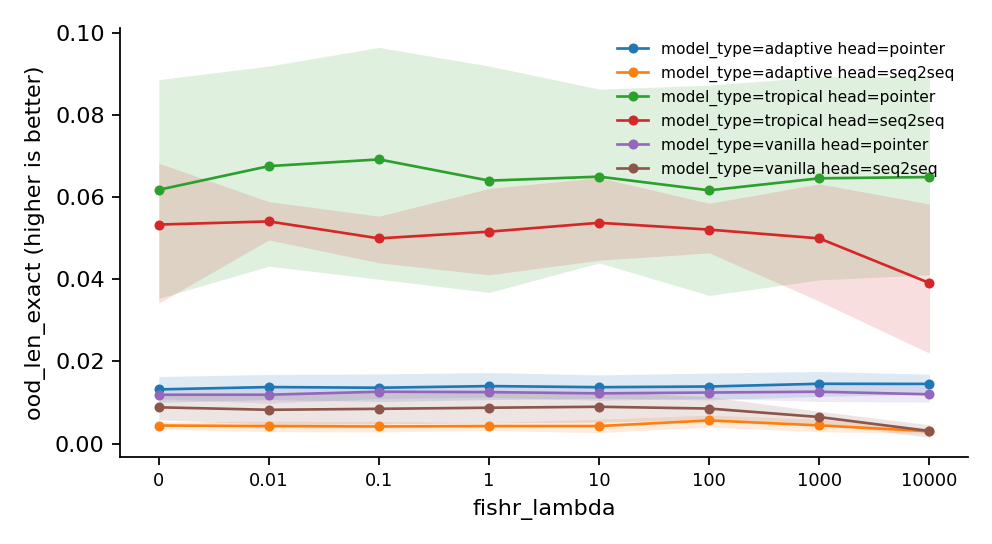
\includegraphics[width=\textwidth]{metric_ood_len_exact.png}
\caption{\texttt{ood\_len\_exact} against \texttt{fishr\_lambda}: the mean over seeds with a 95\% bootstrap CI, one line per combination of the other factors.}
\label{fig:ood_len_exact}
\end{figure}

{\small
\begin{longtable}{lllrlrrr}
\caption{\texttt{ood\_len\_exact} per cell: mean, 95\% bootstrap CI, SD, seeds, diverged runs.}\label{tab:summary-ood_len_exact}\\
\toprule
\texttt{model\_type} & \texttt{head} & \texttt{fishr\_lambda} & mean & 95\% CI & SD & $n$ & div.\\
\midrule
\endhead
adaptive & pointer & 0 & 0.0132 & [0.0101, 0.0163] & 0.00408 & 5 & 0\\
adaptive & pointer & 0.01 & 0.01377 & [0.0107, 0.0168] & 0.00385 & 5 & 0\\
adaptive & pointer & 0.1 & 0.0136 & [0.0102, 0.017] & 0.00424 & 5 & 0\\
adaptive & pointer & 1 & 0.014 & [0.0107, 0.0173] & 0.00425 & 5 & 0\\
adaptive & pointer & 10 & 0.01373 & [0.011, 0.0167] & 0.00378 & 5 & 0\\
adaptive & pointer & 100 & 0.0139 & [0.0106, 0.0172] & 0.00411 & 5 & 0\\
adaptive & pointer & 1000 & 0.01457 & [0.0115, 0.0176] & 0.00403 & 5 & 0\\
adaptive & pointer & 1e+04 & 0.01453 & [0.0121, 0.0169] & 0.0032 & 5 & 0\\
adaptive & seq2seq & 0 & 0.0044 & [0.00353, 0.00527] & 0.00113 & 5 & 0\\
adaptive & seq2seq & 0.01 & 0.004267 & [0.0029, 0.0055] & 0.00173 & 5 & 0\\
adaptive & seq2seq & 0.1 & 0.004167 & [0.00283, 0.0054] & 0.00163 & 5 & 0\\
adaptive & seq2seq & 1 & 0.004267 & [0.0032, 0.0051] & 0.00118 & 5 & 0\\
adaptive & seq2seq & 10 & 0.004267 & [0.00267, 0.00597] & 0.00208 & 5 & 0\\
adaptive & seq2seq & 100 & 0.005633 & [0.004, 0.00693] & 0.00182 & 5 & 0\\
adaptive & seq2seq & 1000 & 0.004433 & [0.0029, 0.00593] & 0.00191 & 5 & 0\\
adaptive & seq2seq & 1e+04 & 0.003 & [0.00247, 0.00363] & $7.26\times10^{-4}$ & 5 & 0\\
tropical & pointer & 0 & 0.0618 & [0.0354, 0.0886] & 0.0352 & 5 & 0\\
tropical & pointer & 0.01 & 0.06757 & [0.0432, 0.0919] & 0.0319 & 5 & 0\\
tropical & pointer & 0.1 & 0.0692 & [0.04, 0.0965] & 0.037 & 5 & 0\\
tropical & pointer & 1 & 0.06403 & [0.0368, 0.0919] & 0.035 & 5 & 0\\
tropical & pointer & 10 & 0.065 & [0.044, 0.0863] & 0.0275 & 5 & 0\\
tropical & pointer & 100 & 0.06167 & [0.0361, 0.0873] & 0.033 & 5 & 0\\
tropical & pointer & 1000 & 0.0646 & [0.0399, 0.0893] & 0.0321 & 5 & 0\\
tropical & pointer & 1e+04 & 0.0649 & [0.0411, 0.0893] & 0.0312 & 5 & 0\\
tropical & seq2seq & 0 & 0.05333 & [0.0342, 0.0683] & 0.0217 & 5 & 0\\
tropical & seq2seq & 0.01 & 0.0541 & [0.0496, 0.0589] & 0.00602 & 5 & 0\\
tropical & seq2seq & 0.1 & 0.04997 & [0.044, 0.0554] & 0.00747 & 5 & 0\\
tropical & seq2seq & 1 & 0.0516 & [0.0411, 0.0621] & 0.014 & 5 & 0\\
tropical & seq2seq & 10 & 0.05377 & [0.0447, 0.0648] & 0.0128 & 5 & 0\\
tropical & seq2seq & 100 & 0.0521 & [0.0464, 0.0585] & 0.00804 & 5 & 0\\
tropical & seq2seq & 1000 & 0.04997 & [0.0347, 0.0632] & 0.0173 & 5 & 0\\
tropical & seq2seq & 1e+04 & 0.0391 & [0.022, 0.0583] & 0.0226 & 5 & 0\\
vanilla & pointer & 0 & 0.0119 & [0.0109, 0.0131] & 0.00132 & 5 & 0\\
vanilla & pointer & 0.01 & 0.0119 & [0.00983, 0.0139] & 0.00263 & 5 & 0\\
vanilla & pointer & 0.1 & 0.01263 & [0.0109, 0.0142] & 0.00215 & 5 & 0\\
vanilla & pointer & 1 & 0.01253 & [0.0113, 0.0138] & 0.00163 & 5 & 0\\
vanilla & pointer & 10 & 0.01223 & [0.0105, 0.0137] & 0.00207 & 5 & 0\\
vanilla & pointer & 100 & 0.01243 & [0.0111, 0.0136] & 0.00171 & 5 & 0\\
vanilla & pointer & 1000 & 0.01263 & [0.0103, 0.015] & 0.00311 & 5 & 0\\
vanilla & pointer & 1e+04 & 0.012 & [0.0101, 0.0142] & 0.00268 & 5 & 0\\
vanilla & seq2seq & 0 & 0.008833 & [0.0058, 0.0121] & 0.00407 & 5 & 0\\
vanilla & seq2seq & 0.01 & 0.008233 & [0.0047, 0.0118] & 0.00472 & 5 & 0\\
vanilla & seq2seq & 0.1 & 0.008467 & [0.0048, 0.0128] & 0.00512 & 5 & 0\\
vanilla & seq2seq & 1 & 0.008733 & [0.00507, 0.0124] & 0.00483 & 5 & 0\\
vanilla & seq2seq & 10 & 0.008967 & [0.00523, 0.0127] & 0.00479 & 5 & 0\\
vanilla & seq2seq & 100 & 0.008533 & [0.0058, 0.0114] & 0.00369 & 5 & 0\\
vanilla & seq2seq & 1000 & 0.006467 & [0.00493, 0.00787] & 0.00186 & 5 & 0\\
vanilla & seq2seq & 1e+04 & 0.003067 & [0.0015, 0.0046] & 0.00192 & 5 & 0\\
\bottomrule
\end{longtable}
}

{\small
\begin{longtable}{lllrrrl}
\caption{\texttt{ood\_len\_exact}: each level of \texttt{fishr\_lambda} against its control (0), within each combination of the other factors. rank: Wilcoxon signed-rank by seed, Holm.}\label{tab:control-ood_len_exact}\\
\toprule
\texttt{model\_type} & \texttt{head} & \texttt{fishr\_lambda} & difference & 95\% CI & $p$ & \\
\midrule
\endhead
adaptive & pointer & 0.01 & 0.001167 & [$-5.00\times10^{-4}$, 0.00123] & 1.0000 & \\
adaptive & pointer & 0.1 & $1.667\times10^{-4}$ & [$-7.00\times10^{-4}$, 0.0015] & 1.0000 & \\
adaptive & pointer & 1 & $5.000\times10^{-4}$ & [$3.00\times10^{-4}$, 0.0014] & 0.4375 & \\
adaptive & pointer & 10 & $8.333\times10^{-4}$ & [$-4.67\times10^{-4}$, 0.00137] & 0.9375 & \\
adaptive & pointer & 100 & $8.333\times10^{-4}$ & [$3.33\times10^{-5}$, 0.00134] & 0.7500 & \\
adaptive & pointer & 1000 & 0.001833 & [$4.67\times10^{-4}$, 0.00207] & 0.7500 & \\
adaptive & pointer & 1e+04 & 0.001167 & [$6.67\times10^{-5}$, 0.00263] & 0.7500 & \\
adaptive & seq2seq & 0.01 & $-5.000\times10^{-4}$ & [$-6.33\times10^{-4}$, $5.33\times10^{-4}$] & 1.0000 & \\
adaptive & seq2seq & 0.1 & $-1.667\times10^{-4}$ & [$-6.33\times10^{-4}$, $2.00\times10^{-4}$] & 1.0000 & \\
adaptive & seq2seq & 1 & $-1.667\times10^{-4}$ & [$-2.33\times10^{-4}$, $-3.33\times10^{-5}$] & 1.0000 & \\
adaptive & seq2seq & 10 & $-6.667\times10^{-4}$ & [$-8.00\times10^{-4}$, $9.67\times10^{-4}$] & 1.0000 & \\
adaptive & seq2seq & 100 & 0.001333 & [$4.67\times10^{-4}$, 0.002] & 0.8750 & \\
adaptive & seq2seq & 1000 & 0 & [$-6.67\times10^{-4}$, $9.00\times10^{-4}$] & 1.0000 & \\
adaptive & seq2seq & 1e+04 & -0.001333 & [-0.00233, $-5.00\times10^{-4}$] & 0.8750 & \\
tropical & pointer & 0.01 & 0.006167 & [-0.00117, 0.0133] & 1.0000 & \\
tropical & pointer & 0.1 & 0.01133 & [-0.00307, 0.0179] & 1.0000 & \\
tropical & pointer & 1 & -0.002833 & [-0.00963, 0.0179] & 1.0000 & \\
tropical & pointer & 10 & 0.0025 & [-0.00707, 0.0148] & 1.0000 & \\
tropical & pointer & 100 & $-1.667\times10^{-4}$ & [-0.00644, 0.00753] & 1.0000 & \\
tropical & pointer & 1000 & 0.006833 & [-0.0068, 0.0127] & 1.0000 & \\
tropical & pointer & 1e+04 & 0.004667 & [-0.0095, 0.014] & 1.0000 & \\
tropical & seq2seq & 0.01 & -0.006667 & [-0.0127, 0.0166] & 1.0000 & \\
tropical & seq2seq & 0.1 & -0.01333 & [-0.0174, 0.0139] & 1.0000 & \\
tropical & seq2seq & 1 & -0.0065 & [-0.0161, 0.0145] & 1.0000 & \\
tropical & seq2seq & 10 & -0.004167 & [-0.0131, 0.0176] & 1.0000 & \\
tropical & seq2seq & 100 & -0.009 & [-0.0117, 0.0122] & 1.0000 & \\
tropical & seq2seq & 1000 & -0.005333 & [-0.00673, $8.67\times10^{-4}$] & 1.0000 & \\
tropical & seq2seq & 1e+04 & -0.01617 & [-0.021, -0.00743] & 0.4375 & \\
vanilla & pointer & 0.01 & $1.667\times10^{-4}$ & [-0.0016, 0.00153] & 1.0000 & \\
vanilla & pointer & 0.1 & $1.000\times10^{-3}$ & [$-2.67\times10^{-4}$, 0.0018] & 1.0000 & \\
vanilla & pointer & 1 & $3.333\times10^{-4}$ & [$-2.67\times10^{-4}$, 0.00177] & 1.0000 & \\
vanilla & pointer & 10 & $8.333\times10^{-4}$ & [-0.00103, 0.00127] & 1.0000 & \\
vanilla & pointer & 100 & 0.001333 & [$-8.37\times10^{-4}$, 0.00187] & 1.0000 & \\
vanilla & pointer & 1000 & 0.001833 & [$-9.00\times10^{-4}$, 0.00233] & 1.0000 & \\
vanilla & pointer & 1e+04 & $-1.667\times10^{-4}$ & [-0.00117, 0.00143] & 1.0000 & \\
vanilla & seq2seq & 0.01 & -0.001333 & [-0.00377, 0.00337] & 1.0000 & \\
vanilla & seq2seq & 0.1 & -0.0015 & [-0.00357, 0.00393] & 1.0000 & \\
vanilla & seq2seq & 1 & $-8.333\times10^{-4}$ & [-0.00323, 0.00387] & 1.0000 & \\
vanilla & seq2seq & 10 & -0.001 & [-0.00187, 0.0032] & 1.0000 & \\
vanilla & seq2seq & 100 & $-3.333\times10^{-4}$ & [-0.00113, $5.33\times10^{-4}$] & 1.0000 & \\
vanilla & seq2seq & 1000 & -0.001667 & [-0.00553, $9.33\times10^{-4}$] & 1.0000 & \\
vanilla & seq2seq & 1e+04 & -0.003 & [-0.00947, -0.00247] & 0.4375 & \\
\bottomrule
\end{longtable}
}

{\small
\begin{longtable}{llrrrrr}
\caption{\texttt{ood\_len\_exact} against log10 \texttt{fishr\_lambda}: rank: Spearman rho, seed-bootstrap CI, with the Jonckheere--Terpstra ordered-trend $\tau$ and $p$.}\label{tab:trend-ood_len_exact}\\
\toprule
\texttt{model\_type} & \texttt{head} & estimate & 95\% CI & $p$ & JT $\tau$ & JT $p$\\
\midrule
\endhead
adaptive & pointer & 0.05381 & [-0.258, 0.32] & 0.7588 & 0.0438 & 0.7375\\
adaptive & seq2seq & -0.131 & [-0.331, 0.0872] & 0.4530 & -0.0971 & 0.4781\\
tropical & pointer & -0.058 & [-0.244, 0.0815] & 0.7407 & -0.0362 & 0.7862\\
tropical & seq2seq & -0.198 & [-0.557, 0.186] & 0.2541 & -0.166 & 0.2282\\
vanilla & pointer & -0.02336 & [-0.151, 0.156] & 0.8940 & -0.00762 & 0.9628\\
vanilla & seq2seq & -0.3411 & [-0.688, 0.0277] & 0.0449 & -0.284 & 0.0312\\
\bottomrule
\end{longtable}
}

{\small
\begin{longtable}{lrrrl}
\caption{\texttt{ood\_len\_exact}: paired contrasts by seed, Holm-corrected across the cells. rank: Wilcoxon signed-rank by seed, Holm.}\label{tab:paired-ood_len_exact}\\
\toprule
contrast (within) & difference & 95\% CI & $p$ & \\
\midrule
\endhead
\stackcell{model\_type: tropical - vanilla\\\footnotesize head=pointer fishr\_lambda=0 } & 0.0499 & [0.00562, 0.0942] & 1.0000 & \\
\stackcell{model\_type: tropical - vanilla\\\footnotesize head=pointer fishr\_lambda=0.01 } & 0.05567 & [0.0163, 0.0951] & 1.0000 & \\
\stackcell{model\_type: tropical - vanilla\\\footnotesize head=pointer fishr\_lambda=0.1 } & 0.05657 & [0.0111, 0.102] & 1.0000 & \\
\stackcell{model\_type: tropical - vanilla\\\footnotesize head=pointer fishr\_lambda=1 } & 0.0515 & [0.0084, 0.0946] & 1.0000 & \\
\stackcell{model\_type: tropical - vanilla\\\footnotesize head=pointer fishr\_lambda=10 } & 0.05277 & [0.0195, 0.086] & 1.0000 & \\
\stackcell{model\_type: tropical - vanilla\\\footnotesize head=pointer fishr\_lambda=100 } & 0.04923 & [0.00859, 0.0899] & 1.0000 & \\
\stackcell{model\_type: tropical - vanilla\\\footnotesize head=pointer fishr\_lambda=1000 } & 0.05197 & [0.0119, 0.092] & 1.0000 & \\
\stackcell{model\_type: tropical - vanilla\\\footnotesize head=pointer fishr\_lambda=1e+04 } & 0.0529 & [0.0141, 0.0917] & 1.0000 & \\
\stackcell{model\_type: tropical - vanilla\\\footnotesize head=seq2seq fishr\_lambda=0 } & 0.0445 & [0.02, 0.069] & 1.0000 & \\
\stackcell{model\_type: tropical - vanilla\\\footnotesize head=seq2seq fishr\_lambda=0.01 } & 0.04587 & [0.0375, 0.0542] & 1.0000 & \\
\stackcell{model\_type: tropical - vanilla\\\footnotesize head=seq2seq fishr\_lambda=0.1 } & 0.0415 & [0.0317, 0.0513] & 1.0000 & \\
\stackcell{model\_type: tropical - vanilla\\\footnotesize head=seq2seq fishr\_lambda=1 } & 0.04287 & [0.0267, 0.059] & 1.0000 & \\
\stackcell{model\_type: tropical - vanilla\\\footnotesize head=seq2seq fishr\_lambda=10 } & 0.0448 & [0.0298, 0.0598] & 1.0000 & \\
\stackcell{model\_type: tropical - vanilla\\\footnotesize head=seq2seq fishr\_lambda=100 } & 0.04357 & [0.0342, 0.0529] & 1.0000 & \\
\stackcell{model\_type: tropical - vanilla\\\footnotesize head=seq2seq fishr\_lambda=1000 } & 0.0435 & [0.0212, 0.0658] & 1.0000 & \\
\stackcell{model\_type: tropical - vanilla\\\footnotesize head=seq2seq fishr\_lambda=1e+04 } & 0.03603 & [0.00969, 0.0624] & 1.0000 & \\
\stackcell{model\_type: adaptive - vanilla\\\footnotesize head=pointer fishr\_lambda=0 } & 0.0013 & [-0.00405, 0.00665] & 1.0000 & \\
\stackcell{model\_type: adaptive - vanilla\\\footnotesize head=pointer fishr\_lambda=0.01 } & 0.001867 & [-0.00345, 0.00719] & 1.0000 & \\
\stackcell{model\_type: adaptive - vanilla\\\footnotesize head=pointer fishr\_lambda=0.1 } & $9.667\times10^{-4}$ & [-0.00461, 0.00655] & 1.0000 & \\
\stackcell{model\_type: adaptive - vanilla\\\footnotesize head=pointer fishr\_lambda=1 } & 0.001467 & [-0.00388, 0.00682] & 1.0000 & \\
\stackcell{model\_type: adaptive - vanilla\\\footnotesize head=pointer fishr\_lambda=10 } & 0.0015 & [-0.00316, 0.00616] & 1.0000 & \\
\stackcell{model\_type: adaptive - vanilla\\\footnotesize head=pointer fishr\_lambda=100 } & 0.001467 & [-0.00332, 0.00625] & 1.0000 & \\
\stackcell{model\_type: adaptive - vanilla\\\footnotesize head=pointer fishr\_lambda=1000 } & 0.001933 & [-0.00419, 0.00806] & 1.0000 & \\
\stackcell{model\_type: adaptive - vanilla\\\footnotesize head=pointer fishr\_lambda=1e+04 } & 0.002533 & [-0.00202, 0.00708] & 1.0000 & \\
\stackcell{model\_type: adaptive - vanilla\\\footnotesize head=seq2seq fishr\_lambda=0 } & -0.004433 & [-0.0104, 0.00155] & 1.0000 & \\
\stackcell{model\_type: adaptive - vanilla\\\footnotesize head=seq2seq fishr\_lambda=0.01 } & -0.003967 & [-0.00967, 0.00173] & 1.0000 & \\
\stackcell{model\_type: adaptive - vanilla\\\footnotesize head=seq2seq fishr\_lambda=0.1 } & -0.0043 & [-0.0106, 0.00203] & 1.0000 & \\
\stackcell{model\_type: adaptive - vanilla\\\footnotesize head=seq2seq fishr\_lambda=1 } & -0.004467 & [-0.0107, 0.00178] & 1.0000 & \\
\stackcell{model\_type: adaptive - vanilla\\\footnotesize head=seq2seq fishr\_lambda=10 } & -0.0047 & [-0.0104, $9.96\times10^{-4}$] & 1.0000 & \\
\stackcell{model\_type: adaptive - vanilla\\\footnotesize head=seq2seq fishr\_lambda=100 } & -0.0029 & [-0.00779, 0.00199] & 1.0000 & \\
\stackcell{model\_type: adaptive - vanilla\\\footnotesize head=seq2seq fishr\_lambda=1000 } & -0.002033 & [-0.00413, $6.39\times10^{-5}$] & 1.0000 & \\
\stackcell{model\_type: adaptive - vanilla\\\footnotesize head=seq2seq fishr\_lambda=1e+04 } & $-6.667\times10^{-5}$ & [-0.00189, 0.00175] & 1.0000 & \\
\stackcell{head: pointer - seq2seq\\\footnotesize model\_type=adaptive fishr\_lambda=0 } & 0.0088 & [0.00268, 0.0149] & 1.0000 & \\
\stackcell{head: pointer - seq2seq\\\footnotesize model\_type=adaptive fishr\_lambda=0.01 } & 0.0095 & [0.00344, 0.0156] & 1.0000 & \\
\stackcell{head: pointer - seq2seq\\\footnotesize model\_type=adaptive fishr\_lambda=0.1 } & 0.009433 & [0.00288, 0.016] & 1.0000 & \\
\stackcell{head: pointer - seq2seq\\\footnotesize model\_type=adaptive fishr\_lambda=1 } & 0.009733 & [0.00344, 0.016] & 1.0000 & \\
\stackcell{head: pointer - seq2seq\\\footnotesize model\_type=adaptive fishr\_lambda=10 } & 0.009467 & [0.00287, 0.0161] & 1.0000 & \\
\stackcell{head: pointer - seq2seq\\\footnotesize model\_type=adaptive fishr\_lambda=100 } & 0.008267 & [0.00202, 0.0145] & 1.0000 & \\
\stackcell{head: pointer - seq2seq\\\footnotesize model\_type=adaptive fishr\_lambda=1000 } & 0.01013 & [0.00322, 0.017] & 1.0000 & \\
\stackcell{head: pointer - seq2seq\\\footnotesize model\_type=adaptive fishr\_lambda=1e+04 } & 0.01153 & [0.00746, 0.0156] & 1.0000 & \\
\stackcell{head: pointer - seq2seq\\\footnotesize model\_type=tropical fishr\_lambda=0 } & 0.008467 & [-0.0399, 0.0568] & 1.0000 & \\
\stackcell{head: pointer - seq2seq\\\footnotesize model\_type=tropical fishr\_lambda=0.01 } & 0.01347 & [-0.027, 0.0539] & 1.0000 & \\
\stackcell{head: pointer - seq2seq\\\footnotesize model\_type=tropical fishr\_lambda=0.1 } & 0.01923 & [-0.0317, 0.0702] & 1.0000 & \\
\stackcell{head: pointer - seq2seq\\\footnotesize model\_type=tropical fishr\_lambda=1 } & 0.01243 & [-0.038, 0.0629] & 1.0000 & \\
\stackcell{head: pointer - seq2seq\\\footnotesize model\_type=tropical fishr\_lambda=10 } & 0.01123 & [-0.0321, 0.0545] & 1.0000 & \\
\stackcell{head: pointer - seq2seq\\\footnotesize model\_type=tropical fishr\_lambda=100 } & 0.009567 & [-0.0342, 0.0533] & 1.0000 & \\
\stackcell{head: pointer - seq2seq\\\footnotesize model\_type=tropical fishr\_lambda=1000 } & 0.01463 & [-0.0246, 0.0539] & 1.0000 & \\
\stackcell{head: pointer - seq2seq\\\footnotesize model\_type=tropical fishr\_lambda=1e+04 } & 0.0258 & [-0.0261, 0.0777] & 1.0000 & \\
\stackcell{head: pointer - seq2seq\\\footnotesize model\_type=vanilla fishr\_lambda=0 } & 0.003067 & [-0.00273, 0.00886] & 1.0000 & \\
\stackcell{head: pointer - seq2seq\\\footnotesize model\_type=vanilla fishr\_lambda=0.01 } & 0.003667 & [-0.002, 0.00933] & 1.0000 & \\
\stackcell{head: pointer - seq2seq\\\footnotesize model\_type=vanilla fishr\_lambda=0.1 } & 0.004167 & [-0.00249, 0.0108] & 1.0000 & \\
\stackcell{head: pointer - seq2seq\\\footnotesize model\_type=vanilla fishr\_lambda=1 } & 0.0038 & [-0.00234, 0.00994] & 1.0000 & \\
\stackcell{head: pointer - seq2seq\\\footnotesize model\_type=vanilla fishr\_lambda=10 } & 0.003267 & [-0.0026, 0.00913] & 1.0000 & \\
\stackcell{head: pointer - seq2seq\\\footnotesize model\_type=vanilla fishr\_lambda=100 } & 0.0039 & [$-7.01\times10^{-4}$, 0.0085] & 1.0000 & \\
\stackcell{head: pointer - seq2seq\\\footnotesize model\_type=vanilla fishr\_lambda=1000 } & 0.006167 & [$1.10\times10^{-4}$, 0.0122] & 1.0000 & \\
\stackcell{head: pointer - seq2seq\\\footnotesize model\_type=vanilla fishr\_lambda=1e+04 } & 0.008933 & [0.00425, 0.0136] & 1.0000 & \\
\bottomrule
\end{longtable}
}

\subsection{\texttt{ood\_val\_f1}}
\begin{figure}[tbp]
\centering
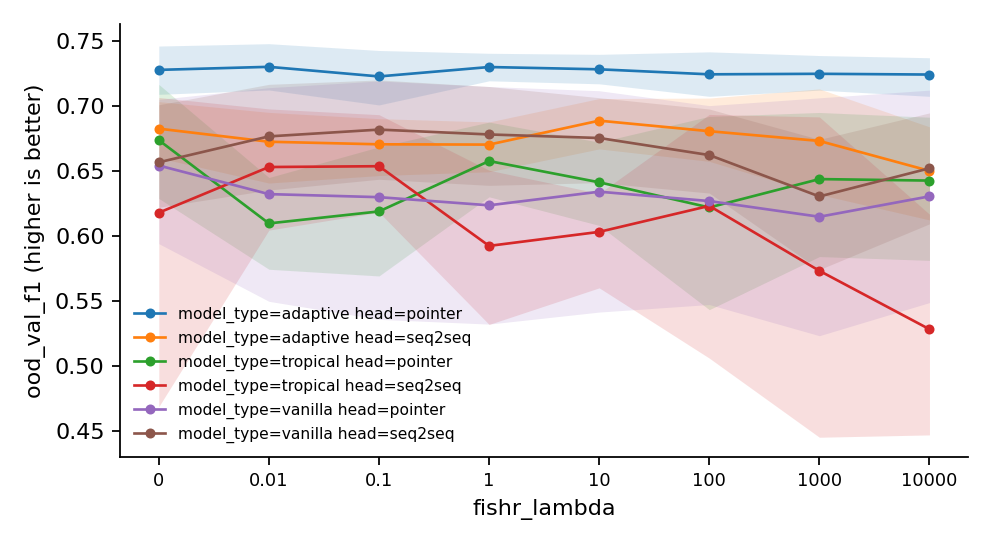
\includegraphics[width=\textwidth]{metric_ood_val_f1.png}
\caption{\texttt{ood\_val\_f1} against \texttt{fishr\_lambda}: the mean over seeds with a 95\% bootstrap CI, one line per combination of the other factors.}
\label{fig:ood_val_f1}
\end{figure}

{\small
\begin{longtable}{lllrlrrr}
\caption{\texttt{ood\_val\_f1} per cell: mean, 95\% bootstrap CI, SD, seeds, diverged runs.}\label{tab:summary-ood_val_f1}\\
\toprule
\texttt{model\_type} & \texttt{head} & \texttt{fishr\_lambda} & mean & 95\% CI & SD & $n$ & div.\\
\midrule
\endhead
adaptive & pointer & 0 & 0.7275 & [0.709, 0.746] & 0.0245 & 5 & 0\\
adaptive & pointer & 0.01 & 0.7298 & [0.712, 0.748] & 0.0224 & 5 & 0\\
adaptive & pointer & 0.1 & 0.7225 & [0.701, 0.742] & 0.0281 & 5 & 0\\
adaptive & pointer & 1 & 0.7297 & [0.719, 0.74] & 0.0143 & 5 & 0\\
adaptive & pointer & 10 & 0.7279 & [0.717, 0.739] & 0.0148 & 5 & 0\\
adaptive & pointer & 100 & 0.7241 & [0.707, 0.741] & 0.0217 & 5 & 0\\
adaptive & pointer & 1000 & 0.7245 & [0.712, 0.739] & 0.0168 & 5 & 0\\
adaptive & pointer & 1e+04 & 0.7239 & [0.707, 0.737] & 0.0192 & 5 & 0\\
adaptive & seq2seq & 0 & 0.6824 & [0.66, 0.703] & 0.0292 & 5 & 0\\
adaptive & seq2seq & 0.01 & 0.6723 & [0.641, 0.695] & 0.0366 & 5 & 0\\
adaptive & seq2seq & 0.1 & 0.6703 & [0.646, 0.69] & 0.0286 & 5 & 0\\
adaptive & seq2seq & 1 & 0.6701 & [0.649, 0.688] & 0.0243 & 5 & 0\\
adaptive & seq2seq & 10 & 0.6885 & [0.667, 0.705] & 0.0258 & 5 & 0\\
adaptive & seq2seq & 100 & 0.6804 & [0.657, 0.706] & 0.0322 & 5 & 0\\
adaptive & seq2seq & 1000 & 0.6729 & [0.632, 0.713] & 0.052 & 5 & 0\\
adaptive & seq2seq & 1e+04 & 0.6499 & [0.612, 0.684] & 0.0473 & 5 & 0\\
tropical & pointer & 0 & 0.6735 & [0.629, 0.716] & 0.058 & 5 & 0\\
tropical & pointer & 0.01 & 0.6096 & [0.574, 0.645] & 0.0476 & 5 & 0\\
tropical & pointer & 0.1 & 0.6188 & [0.569, 0.668] & 0.0623 & 5 & 0\\
tropical & pointer & 1 & 0.6575 & [0.63, 0.687] & 0.0384 & 5 & 0\\
tropical & pointer & 10 & 0.6412 & [0.608, 0.672] & 0.0419 & 5 & 0\\
tropical & pointer & 100 & 0.6219 & [0.543, 0.692] & 0.0974 & 5 & 0\\
tropical & pointer & 1000 & 0.6436 & [0.584, 0.695] & 0.0737 & 5 & 0\\
tropical & pointer & 1e+04 & 0.6425 & [0.581, 0.691] & 0.0649 & 5 & 0\\
tropical & seq2seq & 0 & 0.6178 & [0.469, 0.706] & 0.168 & 5 & 0\\
tropical & seq2seq & 0.01 & 0.6529 & [0.604, 0.698] & 0.0593 & 5 & 0\\
tropical & seq2seq & 0.1 & 0.6535 & [0.618, 0.693] & 0.0488 & 5 & 0\\
tropical & seq2seq & 1 & 0.5923 & [0.532, 0.65] & 0.079 & 5 & 0\\
tropical & seq2seq & 10 & 0.6031 & [0.56, 0.633] & 0.0471 & 5 & 0\\
tropical & seq2seq & 100 & 0.6231 & [0.506, 0.693] & 0.13 & 5 & 0\\
tropical & seq2seq & 1000 & 0.5732 & [0.445, 0.691] & 0.158 & 5 & 0\\
tropical & seq2seq & 1e+04 & 0.5283 & [0.447, 0.617] & 0.108 & 5 & 0\\
vanilla & pointer & 0 & 0.6541 & [0.594, 0.705] & 0.0691 & 5 & 0\\
vanilla & pointer & 0.01 & 0.6321 & [0.55, 0.714] & 0.105 & 5 & 0\\
vanilla & pointer & 0.1 & 0.6298 & [0.536, 0.719] & 0.116 & 5 & 0\\
vanilla & pointer & 1 & 0.6235 & [0.532, 0.715] & 0.115 & 5 & 0\\
vanilla & pointer & 10 & 0.634 & [0.542, 0.711] & 0.105 & 5 & 0\\
vanilla & pointer & 100 & 0.6268 & [0.547, 0.7] & 0.0985 & 5 & 0\\
vanilla & pointer & 1000 & 0.6147 & [0.523, 0.706] & 0.116 & 5 & 0\\
vanilla & pointer & 1e+04 & 0.6304 & [0.549, 0.712] & 0.104 & 5 & 0\\
vanilla & seq2seq & 0 & 0.6565 & [0.622, 0.701] & 0.0512 & 5 & 0\\
vanilla & seq2seq & 0.01 & 0.6764 & [0.635, 0.716] & 0.0535 & 5 & 0\\
vanilla & seq2seq & 0.1 & 0.6816 & [0.643, 0.72] & 0.0495 & 5 & 0\\
vanilla & seq2seq & 1 & 0.6779 & [0.639, 0.715] & 0.0493 & 5 & 0\\
vanilla & seq2seq & 10 & 0.6752 & [0.641, 0.706] & 0.0418 & 5 & 0\\
vanilla & seq2seq & 100 & 0.6621 & [0.633, 0.697] & 0.0415 & 5 & 0\\
vanilla & seq2seq & 1000 & 0.6303 & [0.574, 0.674] & 0.0676 & 5 & 0\\
vanilla & seq2seq & 1e+04 & 0.6519 & [0.609, 0.694] & 0.0551 & 5 & 0\\
\bottomrule
\end{longtable}
}

{\small
\begin{longtable}{lllrrrl}
\caption{\texttt{ood\_val\_f1}: each level of \texttt{fishr\_lambda} against its control (0), within each combination of the other factors. parametric: Dunnett vs control.}\label{tab:control-ood_val_f1}\\
\toprule
\texttt{model\_type} & \texttt{head} & \texttt{fishr\_lambda} & difference & 95\% CI & $p$ & \\
\midrule
\endhead
adaptive & pointer & 0.01 & 0.002339 & [-0.0339, 0.0385] & 1.0000 & \\
adaptive & pointer & 0.1 & -0.005037 & [-0.0412, 0.0312] & 0.9991 & \\
adaptive & pointer & 1 & 0.002188 & [-0.034, 0.0384] & 1.0000 & \\
adaptive & pointer & 10 & $4.367\times10^{-4}$ & [-0.0358, 0.0366] & 1.0000 & \\
adaptive & pointer & 100 & -0.003417 & [-0.0396, 0.0328] & 0.9999 & \\
adaptive & pointer & 1000 & -0.003015 & [-0.0392, 0.0332] & 1.0000 & \\
adaptive & pointer & 1e+04 & -0.003587 & [-0.0398, 0.0326] & 0.9999 & \\
adaptive & seq2seq & 0.01 & -0.01006 & [-0.0726, 0.0524] & 0.9977 & \\
adaptive & seq2seq & 0.1 & -0.01203 & [-0.0745, 0.0505] & 0.9934 & \\
adaptive & seq2seq & 1 & -0.01224 & [-0.0747, 0.0503] & 0.9927 & \\
adaptive & seq2seq & 10 & 0.006134 & [-0.0564, 0.0686] & 0.9999 & \\
adaptive & seq2seq & 100 & -0.001954 & [-0.0645, 0.0605] & 1.0000 & \\
adaptive & seq2seq & 1000 & -0.009445 & [-0.0719, 0.0531] & 0.9984 & \\
adaptive & seq2seq & 1e+04 & -0.03243 & [-0.0949, 0.0301] & 0.5644 & \\
tropical & pointer & 0.01 & -0.06392 & [-0.174, 0.0463] & 0.4509 & \\
tropical & pointer & 0.1 & -0.05472 & [-0.165, 0.0555] & 0.6086 & \\
tropical & pointer & 1 & -0.01603 & [-0.126, 0.0942] & 0.9988 & \\
tropical & pointer & 10 & -0.03235 & [-0.143, 0.0779] & 0.9398 & \\
tropical & pointer & 100 & -0.05167 & [-0.162, 0.0586] & 0.6625 & \\
tropical & pointer & 1000 & -0.02989 & [-0.14, 0.0804] & 0.9585 & \\
tropical & pointer & 1e+04 & -0.03104 & [-0.141, 0.0792] & 0.9503 & \\
tropical & seq2seq & 0.01 & 0.03507 & [-0.156, 0.227] & 0.9950 & \\
tropical & seq2seq & 0.1 & 0.0357 & [-0.156, 0.227] & 0.9945 & \\
tropical & seq2seq & 1 & -0.0255 & [-0.217, 0.166] & 0.9993 & \\
tropical & seq2seq & 10 & -0.01473 & [-0.206, 0.177] & 1.0000 & \\
tropical & seq2seq & 100 & 0.005224 & [-0.186, 0.197] & 1.0000 & \\
tropical & seq2seq & 1000 & -0.0446 & [-0.236, 0.147] & 0.9808 & \\
tropical & seq2seq & 1e+04 & -0.08949 & [-0.281, 0.102] & 0.6652 & \\
vanilla & pointer & 0.01 & -0.02196 & [-0.205, 0.161] & 0.9996 & \\
vanilla & pointer & 0.1 & -0.0243 & [-0.207, 0.158] & 0.9993 & \\
vanilla & pointer & 1 & -0.03056 & [-0.213, 0.152] & 0.9971 & \\
vanilla & pointer & 10 & -0.0201 & [-0.203, 0.163] & 0.9998 & \\
vanilla & pointer & 100 & -0.02729 & [-0.21, 0.155] & 0.9985 & \\
vanilla & pointer & 1000 & -0.03935 & [-0.222, 0.143] & 0.9874 & \\
vanilla & pointer & 1e+04 & -0.02368 & [-0.206, 0.159] & 0.9994 & \\
vanilla & seq2seq & 0.01 & 0.0199 & [-0.0706, 0.11] & 0.9859 & \\
vanilla & seq2seq & 0.1 & 0.02511 & [-0.0653, 0.116] & 0.9536 & \\
vanilla & seq2seq & 1 & 0.02138 & [-0.0691, 0.112] & 0.9793 & \\
vanilla & seq2seq & 10 & 0.01866 & [-0.0718, 0.109] & 0.9901 & \\
vanilla & seq2seq & 100 & 0.00555 & [-0.0849, 0.096] & 1.0000 & \\
vanilla & seq2seq & 1000 & -0.02624 & [-0.117, 0.0642] & 0.9428 & \\
vanilla & seq2seq & 1e+04 & -0.004593 & [-0.095, 0.0859] & 1.0000 & \\
\bottomrule
\end{longtable}
}

{\small
\begin{longtable}{llrrrrr}
\caption{\texttt{ood\_val\_f1} against log10 \texttt{fishr\_lambda}: parametric: OLS slope t-test, seed-bootstrap CI, with the Jonckheere--Terpstra ordered-trend $\tau$ and $p$.}\label{tab:trend-ood_val_f1}\\
\toprule
\texttt{model\_type} & \texttt{head} & estimate & 95\% CI & $p$ & JT $\tau$ & JT $p$\\
\midrule
\endhead
adaptive & pointer & $-6.907\times10^{-4}$ & [-0.00175, $6.53\times10^{-4}$] & 0.6650 & -0.0629 & 0.6371\\
adaptive & seq2seq & -0.001845 & [-0.0105, 0.00867] & 0.5412 & -0.0438 & 0.7632\\
tropical & pointer & 0.004023 & [-0.00338, 0.0106] & 0.4363 & 0.15 & 0.2649\\
tropical & seq2seq & -0.01798 & [-0.0343, -0.00171] & 0.0289 & -0.189 & 0.1554\\
vanilla & pointer & -0.001142 & [-0.00352, 0.00166] & 0.8936 & -0.0362 & 0.7930\\
vanilla & seq2seq & -0.006857 & [-0.0123, -0.00144] & 0.1069 & -0.177 & 0.1850\\
\bottomrule
\end{longtable}
}

{\small
\begin{longtable}{lrrrl}
\caption{\texttt{ood\_val\_f1}: paired contrasts by seed, Holm-corrected across the cells. parametric: paired t-test by seed, Holm.}\label{tab:paired-ood_val_f1}\\
\toprule
contrast (within) & difference & 95\% CI & $p$ & \\
\midrule
\endhead
\stackcell{model\_type: tropical - vanilla\\\footnotesize head=pointer fishr\_lambda=0 } & 0.01946 & [-0.0726, 0.112] & 1.0000 & \\
\stackcell{model\_type: tropical - vanilla\\\footnotesize head=pointer fishr\_lambda=0.01 } & -0.0225 & [-0.189, 0.144] & 1.0000 & \\
\stackcell{model\_type: tropical - vanilla\\\footnotesize head=pointer fishr\_lambda=0.1 } & -0.01095 & [-0.171, 0.149] & 1.0000 & \\
\stackcell{model\_type: tropical - vanilla\\\footnotesize head=pointer fishr\_lambda=1 } & 0.03399 & [-0.112, 0.18] & 1.0000 & \\
\stackcell{model\_type: tropical - vanilla\\\footnotesize head=pointer fishr\_lambda=10 } & 0.00722 & [-0.102, 0.116] & 1.0000 & \\
\stackcell{model\_type: tropical - vanilla\\\footnotesize head=pointer fishr\_lambda=100 } & -0.004914 & [-0.16, 0.15] & 1.0000 & \\
\stackcell{model\_type: tropical - vanilla\\\footnotesize head=pointer fishr\_lambda=1000 } & 0.02893 & [-0.124, 0.181] & 1.0000 & \\
\stackcell{model\_type: tropical - vanilla\\\footnotesize head=pointer fishr\_lambda=1e+04 } & 0.0121 & [-0.133, 0.157] & 1.0000 & \\
\stackcell{model\_type: tropical - vanilla\\\footnotesize head=seq2seq fishr\_lambda=0 } & -0.0387 & [-0.212, 0.135] & 1.0000 & \\
\stackcell{model\_type: tropical - vanilla\\\footnotesize head=seq2seq fishr\_lambda=0.01 } & -0.02353 & [-0.123, 0.0763] & 1.0000 & \\
\stackcell{model\_type: tropical - vanilla\\\footnotesize head=seq2seq fishr\_lambda=0.1 } & -0.02811 & [-0.124, 0.0679] & 1.0000 & \\
\stackcell{model\_type: tropical - vanilla\\\footnotesize head=seq2seq fishr\_lambda=1 } & -0.08558 & [-0.195, 0.0234] & 1.0000 & \\
\stackcell{model\_type: tropical - vanilla\\\footnotesize head=seq2seq fishr\_lambda=10 } & -0.07209 & [-0.149, 0.00445] & 0.9251 & \\
\stackcell{model\_type: tropical - vanilla\\\footnotesize head=seq2seq fishr\_lambda=100 } & -0.03902 & [-0.189, 0.111] & 1.0000 & \\
\stackcell{model\_type: tropical - vanilla\\\footnotesize head=seq2seq fishr\_lambda=1000 } & -0.05706 & [-0.222, 0.108] & 1.0000 & \\
\stackcell{model\_type: tropical - vanilla\\\footnotesize head=seq2seq fishr\_lambda=1e+04 } & -0.1236 & [-0.254, 0.00658] & 0.9251 & \\
\stackcell{model\_type: adaptive - vanilla\\\footnotesize head=pointer fishr\_lambda=0 } & 0.07344 & [-0.0176, 0.164] & 1.0000 & \\
\stackcell{model\_type: adaptive - vanilla\\\footnotesize head=pointer fishr\_lambda=0.01 } & 0.09774 & [-0.0312, 0.227] & 1.0000 & \\
\stackcell{model\_type: adaptive - vanilla\\\footnotesize head=pointer fishr\_lambda=0.1 } & 0.0927 & [-0.053, 0.238] & 1.0000 & \\
\stackcell{model\_type: adaptive - vanilla\\\footnotesize head=pointer fishr\_lambda=1 } & 0.1062 & [-0.0383, 0.251] & 1.0000 & \\
\stackcell{model\_type: adaptive - vanilla\\\footnotesize head=pointer fishr\_lambda=10 } & 0.09398 & [-0.0324, 0.22] & 1.0000 & \\
\stackcell{model\_type: adaptive - vanilla\\\footnotesize head=pointer fishr\_lambda=100 } & 0.09732 & [-0.0212, 0.216] & 1.0000 & \\
\stackcell{model\_type: adaptive - vanilla\\\footnotesize head=pointer fishr\_lambda=1000 } & 0.1098 & [-0.0311, 0.251] & 1.0000 & \\
\stackcell{model\_type: adaptive - vanilla\\\footnotesize head=pointer fishr\_lambda=1e+04 } & 0.09353 & [-0.0397, 0.227] & 1.0000 & \\
\stackcell{model\_type: adaptive - vanilla\\\footnotesize head=seq2seq fishr\_lambda=0 } & 0.02584 & [-0.0448, 0.0965] & 1.0000 & \\
\stackcell{model\_type: adaptive - vanilla\\\footnotesize head=seq2seq fishr\_lambda=0.01 } & -0.004114 & [-0.101, 0.0927] & 1.0000 & \\
\stackcell{model\_type: adaptive - vanilla\\\footnotesize head=seq2seq fishr\_lambda=0.1 } & -0.01129 & [-0.0887, 0.0661] & 1.0000 & \\
\stackcell{model\_type: adaptive - vanilla\\\footnotesize head=seq2seq fishr\_lambda=1 } & -0.007781 & [-0.088, 0.0725] & 1.0000 & \\
\stackcell{model\_type: adaptive - vanilla\\\footnotesize head=seq2seq fishr\_lambda=10 } & 0.01332 & [-0.0226, 0.0492] & 1.0000 & \\
\stackcell{model\_type: adaptive - vanilla\\\footnotesize head=seq2seq fishr\_lambda=100 } & 0.01834 & [-0.0177, 0.0543] & 1.0000 & \\
\stackcell{model\_type: adaptive - vanilla\\\footnotesize head=seq2seq fishr\_lambda=1000 } & 0.04264 & [-0.0353, 0.121] & 1.0000 & \\
\stackcell{model\_type: adaptive - vanilla\\\footnotesize head=seq2seq fishr\_lambda=1e+04 } & -0.001997 & [-0.0517, 0.0477] & 1.0000 & \\
\stackcell{head: pointer - seq2seq\\\footnotesize model\_type=adaptive fishr\_lambda=0 } & 0.04513 & [0.00707, 0.0832] & 0.6934 & \\
\stackcell{head: pointer - seq2seq\\\footnotesize model\_type=adaptive fishr\_lambda=0.01 } & 0.05753 & [0.00845, 0.107] & 0.6934 & \\
\stackcell{head: pointer - seq2seq\\\footnotesize model\_type=adaptive fishr\_lambda=0.1 } & 0.05212 & [-0.00209, 0.106] & 1.0000 & \\
\stackcell{head: pointer - seq2seq\\\footnotesize model\_type=adaptive fishr\_lambda=1 } & 0.05956 & [0.0239, 0.0953] & 0.2352 & \\
\stackcell{head: pointer - seq2seq\\\footnotesize model\_type=adaptive fishr\_lambda=10 } & 0.03943 & [-0.00848, 0.0873] & 1.0000 & \\
\stackcell{head: pointer - seq2seq\\\footnotesize model\_type=adaptive fishr\_lambda=100 } & 0.04367 & [-0.005, 0.0923] & 1.0000 & \\
\stackcell{head: pointer - seq2seq\\\footnotesize model\_type=adaptive fishr\_lambda=1000 } & 0.05156 & [-0.0254, 0.129] & 1.0000 & \\
\stackcell{head: pointer - seq2seq\\\footnotesize model\_type=adaptive fishr\_lambda=1e+04 } & 0.07397 & [0.0061, 0.142] & 0.8177 & \\
\stackcell{head: pointer - seq2seq\\\footnotesize model\_type=tropical fishr\_lambda=0 } & 0.05569 & [-0.15, 0.261] & 1.0000 & \\
\stackcell{head: pointer - seq2seq\\\footnotesize model\_type=tropical fishr\_lambda=0.01 } & -0.0433 & [-0.162, 0.0755] & 1.0000 & \\
\stackcell{head: pointer - seq2seq\\\footnotesize model\_type=tropical fishr\_lambda=0.1 } & -0.03472 & [-0.156, 0.0866] & 1.0000 & \\
\stackcell{head: pointer - seq2seq\\\footnotesize model\_type=tropical fishr\_lambda=1 } & 0.06517 & [-0.0483, 0.179] & 1.0000 & \\
\stackcell{head: pointer - seq2seq\\\footnotesize model\_type=tropical fishr\_lambda=10 } & 0.03808 & [-0.0342, 0.11] & 1.0000 & \\
\stackcell{head: pointer - seq2seq\\\footnotesize model\_type=tropical fishr\_lambda=100 } & -0.001205 & [-0.252, 0.25] & 1.0000 & \\
\stackcell{head: pointer - seq2seq\\\footnotesize model\_type=tropical fishr\_lambda=1000 } & 0.07041 & [-0.149, 0.29] & 1.0000 & \\
\stackcell{head: pointer - seq2seq\\\footnotesize model\_type=tropical fishr\_lambda=1e+04 } & 0.1141 & [-0.0805, 0.309] & 1.0000 & \\
\stackcell{head: pointer - seq2seq\\\footnotesize model\_type=vanilla fishr\_lambda=0 } & -0.002468 & [-0.0413, 0.0364] & 1.0000 & \\
\stackcell{head: pointer - seq2seq\\\footnotesize model\_type=vanilla fishr\_lambda=0.01 } & -0.04433 & [-0.18, 0.0912] & 1.0000 & \\
\stackcell{head: pointer - seq2seq\\\footnotesize model\_type=vanilla fishr\_lambda=0.1 } & -0.05188 & [-0.204, 0.1] & 1.0000 & \\
\stackcell{head: pointer - seq2seq\\\footnotesize model\_type=vanilla fishr\_lambda=1 } & -0.0544 & [-0.202, 0.0928] & 1.0000 & \\
\stackcell{head: pointer - seq2seq\\\footnotesize model\_type=vanilla fishr\_lambda=10 } & -0.04123 & [-0.184, 0.102] & 1.0000 & \\
\stackcell{head: pointer - seq2seq\\\footnotesize model\_type=vanilla fishr\_lambda=100 } & -0.03531 & [-0.146, 0.0755] & 1.0000 & \\
\stackcell{head: pointer - seq2seq\\\footnotesize model\_type=vanilla fishr\_lambda=1000 } & -0.01558 & [-0.155, 0.124] & 1.0000 & \\
\stackcell{head: pointer - seq2seq\\\footnotesize model\_type=vanilla fishr\_lambda=1e+04 } & -0.02155 & [-0.176, 0.132] & 1.0000 & \\
\bottomrule
\end{longtable}
}

\subsection{\texttt{ood\_val\_exact}}
\begin{figure}[tbp]
\centering
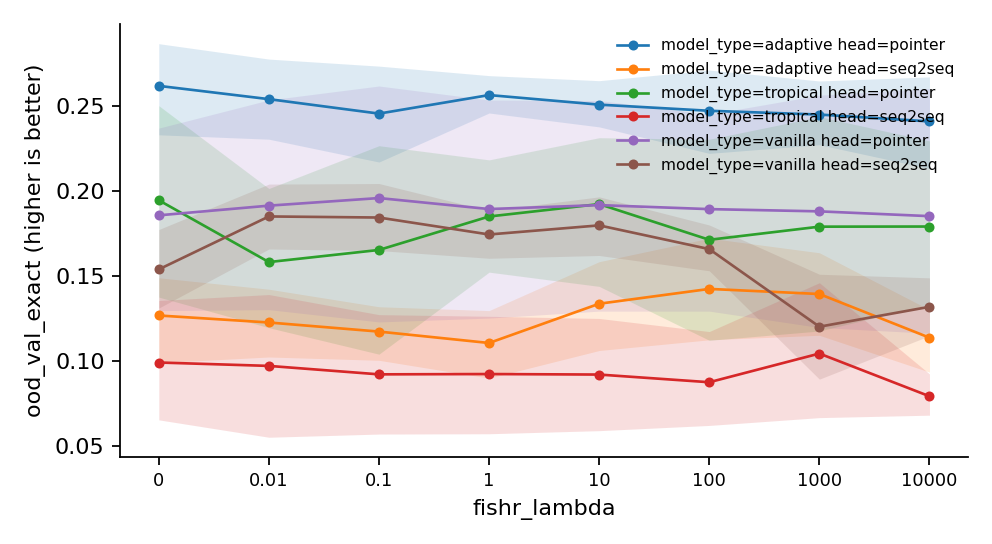
\includegraphics[width=\textwidth]{metric_ood_val_exact.png}
\caption{\texttt{ood\_val\_exact} against \texttt{fishr\_lambda}: the mean over seeds with a 95\% bootstrap CI, one line per combination of the other factors.}
\label{fig:ood_val_exact}
\end{figure}

{\small
\begin{longtable}{lllrlrrr}
\caption{\texttt{ood\_val\_exact} per cell: mean, 95\% bootstrap CI, SD, seeds, diverged runs.}\label{tab:summary-ood_val_exact}\\
\toprule
\texttt{model\_type} & \texttt{head} & \texttt{fishr\_lambda} & mean & 95\% CI & SD & $n$ & div.\\
\midrule
\endhead
adaptive & pointer & 0 & 0.2621 & [0.233, 0.287] & 0.035 & 5 & 0\\
adaptive & pointer & 0.01 & 0.2542 & [0.231, 0.278] & 0.032 & 5 & 0\\
adaptive & pointer & 0.1 & 0.2457 & [0.217, 0.274] & 0.0374 & 5 & 0\\
adaptive & pointer & 1 & 0.2566 & [0.246, 0.268] & 0.0144 & 5 & 0\\
adaptive & pointer & 10 & 0.251 & [0.238, 0.265] & 0.0178 & 5 & 0\\
adaptive & pointer & 100 & 0.2474 & [0.222, 0.271] & 0.0316 & 5 & 0\\
adaptive & pointer & 1000 & 0.2452 & [0.227, 0.265] & 0.0238 & 5 & 0\\
adaptive & pointer & 1e+04 & 0.2411 & [0.213, 0.267] & 0.033 & 5 & 0\\
adaptive & seq2seq & 0 & 0.1268 & [0.0989, 0.149] & 0.0326 & 5 & 0\\
adaptive & seq2seq & 0.01 & 0.1226 & [0.102, 0.142] & 0.0258 & 5 & 0\\
adaptive & seq2seq & 0.1 & 0.1173 & [0.1, 0.132] & 0.0204 & 5 & 0\\
adaptive & seq2seq & 1 & 0.1106 & [0.0898, 0.13] & 0.0237 & 5 & 0\\
adaptive & seq2seq & 10 & 0.1337 & [0.106, 0.158] & 0.0319 & 5 & 0\\
adaptive & seq2seq & 100 & 0.1424 & [0.112, 0.172] & 0.0398 & 5 & 0\\
adaptive & seq2seq & 1000 & 0.1394 & [0.115, 0.164] & 0.0325 & 5 & 0\\
adaptive & seq2seq & 1e+04 & 0.1137 & [0.0934, 0.13] & 0.0234 & 5 & 0\\
tropical & pointer & 0 & 0.1947 & [0.138, 0.25] & 0.0709 & 5 & 0\\
tropical & pointer & 0.01 & 0.1582 & [0.12, 0.202] & 0.0524 & 5 & 0\\
tropical & pointer & 0.1 & 0.1654 & [0.104, 0.227] & 0.0787 & 5 & 0\\
tropical & pointer & 1 & 0.1851 & [0.152, 0.218] & 0.045 & 5 & 0\\
tropical & pointer & 10 & 0.1924 & [0.144, 0.232] & 0.058 & 5 & 0\\
tropical & pointer & 100 & 0.1714 & [0.112, 0.231] & 0.0758 & 5 & 0\\
tropical & pointer & 1000 & 0.1791 & [0.118, 0.244] & 0.0784 & 5 & 0\\
tropical & pointer & 1e+04 & 0.1792 & [0.133, 0.23] & 0.0637 & 5 & 0\\
tropical & seq2seq & 0 & 0.09906 & [0.0653, 0.136] & 0.0461 & 5 & 0\\
tropical & seq2seq & 0.01 & 0.09706 & [0.055, 0.139] & 0.0538 & 5 & 0\\
tropical & seq2seq & 0.1 & 0.09208 & [0.0569, 0.127] & 0.0453 & 5 & 0\\
tropical & seq2seq & 1 & 0.09226 & [0.0571, 0.126] & 0.0452 & 5 & 0\\
tropical & seq2seq & 10 & 0.09196 & [0.0589, 0.125] & 0.0416 & 5 & 0\\
tropical & seq2seq & 100 & 0.08744 & [0.062, 0.117] & 0.0353 & 5 & 0\\
tropical & seq2seq & 1000 & 0.1043 & [0.0666, 0.146] & 0.0538 & 5 & 0\\
tropical & seq2seq & 1e+04 & 0.07918 & [0.068, 0.0924] & 0.0151 & 5 & 0\\
vanilla & pointer & 0 & 0.1858 & [0.13, 0.237] & 0.0653 & 5 & 0\\
vanilla & pointer & 0.01 & 0.1915 & [0.13, 0.254] & 0.0795 & 5 & 0\\
vanilla & pointer & 0.1 & 0.196 & [0.123, 0.262] & 0.0899 & 5 & 0\\
vanilla & pointer & 1 & 0.1895 & [0.125, 0.254] & 0.0824 & 5 & 0\\
vanilla & pointer & 10 & 0.1918 & [0.129, 0.253] & 0.0794 & 5 & 0\\
vanilla & pointer & 100 & 0.1894 & [0.129, 0.245] & 0.0734 & 5 & 0\\
vanilla & pointer & 1000 & 0.1881 & [0.12, 0.257] & 0.0877 & 5 & 0\\
vanilla & pointer & 1e+04 & 0.1853 & [0.116, 0.26] & 0.0932 & 5 & 0\\
vanilla & seq2seq & 0 & 0.1539 & [0.131, 0.177] & 0.0307 & 5 & 0\\
vanilla & seq2seq & 0.01 & 0.1851 & [0.166, 0.204] & 0.0245 & 5 & 0\\
vanilla & seq2seq & 0.1 & 0.1845 & [0.165, 0.205] & 0.0265 & 5 & 0\\
vanilla & seq2seq & 1 & 0.1745 & [0.16, 0.189] & 0.0183 & 5 & 0\\
vanilla & seq2seq & 10 & 0.1799 & [0.162, 0.197] & 0.0224 & 5 & 0\\
vanilla & seq2seq & 100 & 0.1659 & [0.153, 0.18] & 0.0175 & 5 & 0\\
vanilla & seq2seq & 1000 & 0.1202 & [0.0893, 0.151] & 0.0407 & 5 & 0\\
vanilla & seq2seq & 1e+04 & 0.1319 & [0.115, 0.149] & 0.0219 & 5 & 0\\
\bottomrule
\end{longtable}
}

{\small
\begin{longtable}{lllrrrl}
\caption{\texttt{ood\_val\_exact}: each level of \texttt{fishr\_lambda} against its control (0), within each combination of the other factors. parametric: Dunnett vs control.}\label{tab:control-ood_val_exact}\\
\toprule
\texttt{model\_type} & \texttt{head} & \texttt{fishr\_lambda} & difference & 95\% CI & $p$ & \\
\midrule
\endhead
adaptive & pointer & 0.01 & -0.00782 & [-0.0589, 0.0432] & 0.9983 & \\
adaptive & pointer & 0.1 & -0.01634 & [-0.0674, 0.0347] & 0.9114 & \\
adaptive & pointer & 1 & -0.00542 & [-0.0565, 0.0456] & 0.9998 & \\
adaptive & pointer & 10 & -0.01106 & [-0.0621, 0.04] & 0.9870 & \\
adaptive & pointer & 100 & -0.01468 & [-0.0657, 0.0364] & 0.9450 & \\
adaptive & pointer & 1000 & -0.0169 & [-0.0679, 0.0341] & 0.8978 & \\
adaptive & pointer & 1e+04 & -0.02094 & [-0.072, 0.0301] & 0.7736 & \\
adaptive & seq2seq & 0.01 & -0.00412 & [-0.0555, 0.0472] & 1.0000 & \\
adaptive & seq2seq & 0.1 & -0.00948 & [-0.0608, 0.0419] & 0.9948 & \\
adaptive & seq2seq & 1 & -0.0162 & [-0.0675, 0.0351] & 0.9167 & \\
adaptive & seq2seq & 10 & 0.00694 & [-0.0444, 0.0583] & 0.9992 & \\
adaptive & seq2seq & 100 & 0.01566 & [-0.0357, 0.067] & 0.9282 & \\
adaptive & seq2seq & 1000 & 0.01266 & [-0.0387, 0.064] & 0.9742 & \\
adaptive & seq2seq & 1e+04 & -0.01306 & [-0.0644, 0.0383] & 0.9698 & \\
tropical & pointer & 0.01 & -0.03642 & [-0.152, 0.0796] & 0.9186 & \\
tropical & pointer & 0.1 & -0.02928 & [-0.145, 0.0868] & 0.9710 & \\
tropical & pointer & 1 & -0.00956 & [-0.126, 0.106] & 1.0000 & \\
tropical & pointer & 10 & -0.00226 & [-0.118, 0.114] & 1.0000 & \\
tropical & pointer & 100 & -0.0233 & [-0.139, 0.0927] & 0.9915 & \\
tropical & pointer & 1000 & -0.01556 & [-0.132, 0.1] & 0.9993 & \\
tropical & pointer & 1e+04 & -0.01548 & [-0.132, 0.101] & 0.9993 & \\
tropical & seq2seq & 0.01 & -0.002 & [-0.0782, 0.0742] & 1.0000 & \\
tropical & seq2seq & 0.1 & -0.00698 & [-0.0831, 0.0692] & 0.9999 & \\
tropical & seq2seq & 1 & -0.0068 & [-0.083, 0.0694] & 0.9999 & \\
tropical & seq2seq & 10 & -0.0071 & [-0.0833, 0.0691] & 0.9999 & \\
tropical & seq2seq & 100 & -0.01162 & [-0.0878, 0.0645] & 0.9984 & \\
tropical & seq2seq & 1000 & 0.00528 & [-0.0709, 0.0814] & 1.0000 & \\
tropical & seq2seq & 1e+04 & -0.01988 & [-0.096, 0.0563] & 0.9656 & \\
vanilla & pointer & 0.01 & 0.0057 & [-0.137, 0.149] & 1.0000 & \\
vanilla & pointer & 0.1 & 0.01018 & [-0.133, 0.153] & 1.0000 & \\
vanilla & pointer & 1 & 0.0037 & [-0.139, 0.147] & 1.0000 & \\
vanilla & pointer & 10 & 0.00602 & [-0.137, 0.149] & 1.0000 & \\
vanilla & pointer & 100 & 0.00366 & [-0.139, 0.147] & 1.0000 & \\
vanilla & pointer & 1000 & 0.00234 & [-0.141, 0.145] & 1.0000 & \\
vanilla & pointer & 1e+04 & $-4.800\times10^{-4}$ & [-0.143, 0.142] & 1.0000 & \\
vanilla & seq2seq & 0.01 & 0.03118 & [-0.0147, 0.0771] & 0.2944 & \\
vanilla & seq2seq & 0.1 & 0.03054 & [-0.0154, 0.0765] & 0.3137 & \\
vanilla & seq2seq & 1 & 0.02056 & [-0.0254, 0.0665] & 0.7033 & \\
vanilla & seq2seq & 10 & 0.02592 & [-0.02, 0.0718] & 0.4784 & \\
vanilla & seq2seq & 100 & 0.01194 & [-0.034, 0.0579] & 0.9662 & \\
vanilla & seq2seq & 1000 & -0.03378 & [-0.0797, 0.0121] & 0.2241 & \\
vanilla & seq2seq & 1e+04 & -0.02206 & [-0.068, 0.0239] & 0.6396 & \\
\bottomrule
\end{longtable}
}

{\small
\begin{longtable}{llrrrrr}
\caption{\texttt{ood\_val\_exact} against log10 \texttt{fishr\_lambda}: parametric: OLS slope t-test, seed-bootstrap CI, with the Jonckheere--Terpstra ordered-trend $\tau$ and $p$.}\label{tab:trend-ood_val_exact}\\
\toprule
\texttt{model\_type} & \texttt{head} & estimate & 95\% CI & $p$ & JT $\tau$ & JT $p$\\
\midrule
\endhead
adaptive & pointer & -0.001776 & [-0.00274, $-1.68\times10^{-4}$] & 0.4302 & -0.131 & 0.3229\\
adaptive & seq2seq & 0.001761 & [$-8.20\times10^{-4}$, 0.00409] & 0.4785 & 0.101 & 0.4587\\
tropical & pointer & 0.002733 & [-0.00406, 0.01] & 0.6017 & 0.12 & 0.3749\\
tropical & seq2seq & -0.001212 & [-0.00607, 0.00452] & 0.7250 & -0.0324 & 0.8206\\
vanilla & pointer & -0.001224 & [-0.00277, $5.44\times10^{-4}$] & 0.8526 & -0.0533 & 0.6973\\
vanilla & seq2seq & -0.01061 & [-0.0168, -0.00455] & $<10^{-4}$ & -0.493 & 0.0004\\
\bottomrule
\end{longtable}
}

{\small
\begin{longtable}{lrrrl}
\caption{\texttt{ood\_val\_exact}: paired contrasts by seed, Holm-corrected across the cells. parametric: paired t-test by seed, Holm.}\label{tab:paired-ood_val_exact}\\
\toprule
contrast (within) & difference & 95\% CI & $p$ & \\
\midrule
\endhead
\stackcell{model\_type: tropical - vanilla\\\footnotesize head=pointer fishr\_lambda=0 } & 0.00888 & [-0.0926, 0.11] & 1.0000 & \\
\stackcell{model\_type: tropical - vanilla\\\footnotesize head=pointer fishr\_lambda=0.01 } & -0.03324 & [-0.167, 0.101] & 1.0000 & \\
\stackcell{model\_type: tropical - vanilla\\\footnotesize head=pointer fishr\_lambda=0.1 } & -0.03058 & [-0.171, 0.11] & 1.0000 & \\
\stackcell{model\_type: tropical - vanilla\\\footnotesize head=pointer fishr\_lambda=1 } & -0.00438 & [-0.109, 0.0997] & 1.0000 & \\
\stackcell{model\_type: tropical - vanilla\\\footnotesize head=pointer fishr\_lambda=10 } & $6.000\times10^{-4}$ & [-0.102, 0.103] & 1.0000 & \\
\stackcell{model\_type: tropical - vanilla\\\footnotesize head=pointer fishr\_lambda=100 } & -0.01808 & [-0.125, 0.0887] & 1.0000 & \\
\stackcell{model\_type: tropical - vanilla\\\footnotesize head=pointer fishr\_lambda=1000 } & -0.00902 & [-0.14, 0.121] & 1.0000 & \\
\stackcell{model\_type: tropical - vanilla\\\footnotesize head=pointer fishr\_lambda=1e+04 } & -0.00612 & [-0.0884, 0.0762] & 1.0000 & \\
\stackcell{model\_type: tropical - vanilla\\\footnotesize head=seq2seq fishr\_lambda=0 } & -0.05488 & [-0.117, 0.00684] & 0.6903 & \\
\stackcell{model\_type: tropical - vanilla\\\footnotesize head=seq2seq fishr\_lambda=0.01 } & -0.08806 & [-0.181, 0.00457] & 0.6337 & \\
\stackcell{model\_type: tropical - vanilla\\\footnotesize head=seq2seq fishr\_lambda=0.1 } & -0.0924 & [-0.168, -0.0172] & 0.3241 & \\
\stackcell{model\_type: tropical - vanilla\\\footnotesize head=seq2seq fishr\_lambda=1 } & -0.08224 & [-0.147, -0.0173] & 0.3191 & \\
\stackcell{model\_type: tropical - vanilla\\\footnotesize head=seq2seq fishr\_lambda=10 } & -0.0879 & [-0.156, -0.0201] & 0.3187 & \\
\stackcell{model\_type: tropical - vanilla\\\footnotesize head=seq2seq fishr\_lambda=100 } & -0.07844 & [-0.136, -0.0211] & 0.3055 & \\
\stackcell{model\_type: tropical - vanilla\\\footnotesize head=seq2seq fishr\_lambda=1000 } & -0.01582 & [-0.0709, 0.0393] & 1.0000 & \\
\stackcell{model\_type: tropical - vanilla\\\footnotesize head=seq2seq fishr\_lambda=1e+04 } & -0.0527 & [-0.0923, -0.0131] & 0.3148 & \\
\stackcell{model\_type: adaptive - vanilla\\\footnotesize head=pointer fishr\_lambda=0 } & 0.07628 & [0.00166, 0.151] & 0.6049 & \\
\stackcell{model\_type: adaptive - vanilla\\\footnotesize head=pointer fishr\_lambda=0.01 } & 0.06276 & [-0.0237, 0.149] & 1.0000 & \\
\stackcell{model\_type: adaptive - vanilla\\\footnotesize head=pointer fishr\_lambda=0.1 } & 0.04976 & [-0.0586, 0.158] & 1.0000 & \\
\stackcell{model\_type: adaptive - vanilla\\\footnotesize head=pointer fishr\_lambda=1 } & 0.06716 & [-0.0285, 0.163] & 1.0000 & \\
\stackcell{model\_type: adaptive - vanilla\\\footnotesize head=pointer fishr\_lambda=10 } & 0.0592 & [-0.0299, 0.148] & 1.0000 & \\
\stackcell{model\_type: adaptive - vanilla\\\footnotesize head=pointer fishr\_lambda=100 } & 0.05794 & [-0.0135, 0.129] & 0.8759 & \\
\stackcell{model\_type: adaptive - vanilla\\\footnotesize head=pointer fishr\_lambda=1000 } & 0.05704 & [-0.0403, 0.154] & 1.0000 & \\
\stackcell{model\_type: adaptive - vanilla\\\footnotesize head=pointer fishr\_lambda=1e+04 } & 0.05582 & [-0.055, 0.167] & 1.0000 & \\
\stackcell{model\_type: adaptive - vanilla\\\footnotesize head=seq2seq fishr\_lambda=0 } & -0.02718 & [-0.102, 0.048] & 1.0000 & \\
\stackcell{model\_type: adaptive - vanilla\\\footnotesize head=seq2seq fishr\_lambda=0.01 } & -0.06248 & [-0.123, -0.00155] & 0.6049 & \\
\stackcell{model\_type: adaptive - vanilla\\\footnotesize head=seq2seq fishr\_lambda=0.1 } & -0.0672 & [-0.116, -0.0188] & 0.2922 & \\
\stackcell{model\_type: adaptive - vanilla\\\footnotesize head=seq2seq fishr\_lambda=1 } & -0.06394 & [-0.112, -0.0158] & 0.3165 & \\
\stackcell{model\_type: adaptive - vanilla\\\footnotesize head=seq2seq fishr\_lambda=10 } & -0.04616 & [-0.0983, 0.00599] & 0.7686 & \\
\stackcell{model\_type: adaptive - vanilla\\\footnotesize head=seq2seq fishr\_lambda=100 } & -0.02346 & [-0.0936, 0.0466] & 1.0000 & \\
\stackcell{model\_type: adaptive - vanilla\\\footnotesize head=seq2seq fishr\_lambda=1000 } & 0.01926 & [-0.0325, 0.071] & 1.0000 & \\
\stackcell{model\_type: adaptive - vanilla\\\footnotesize head=seq2seq fishr\_lambda=1e+04 } & -0.01818 & [-0.0352, -0.00117] & 0.5775 & \\
\stackcell{head: pointer - seq2seq\\\footnotesize model\_type=adaptive fishr\_lambda=0 } & 0.1353 & [0.0718, 0.199] & 0.0735 & \\
\stackcell{head: pointer - seq2seq\\\footnotesize model\_type=adaptive fishr\_lambda=0.01 } & 0.1316 & [0.103, 0.161] & 0.0052 & *\\
\stackcell{head: pointer - seq2seq\\\footnotesize model\_type=adaptive fishr\_lambda=0.1 } & 0.1284 & [0.0933, 0.164] & 0.0117 & *\\
\stackcell{head: pointer - seq2seq\\\footnotesize model\_type=adaptive fishr\_lambda=1 } & 0.1461 & [0.116, 0.176] & 0.0042 & *\\
\stackcell{head: pointer - seq2seq\\\footnotesize model\_type=adaptive fishr\_lambda=10 } & 0.1173 & [0.0817, 0.153] & 0.0166 & *\\
\stackcell{head: pointer - seq2seq\\\footnotesize model\_type=adaptive fishr\_lambda=100 } & 0.105 & [0.0424, 0.168] & 0.1634 & \\
\stackcell{head: pointer - seq2seq\\\footnotesize model\_type=adaptive fishr\_lambda=1000 } & 0.1057 & [0.0595, 0.152] & 0.0599 & \\
\stackcell{head: pointer - seq2seq\\\footnotesize model\_type=adaptive fishr\_lambda=1e+04 } & 0.1274 & [0.0779, 0.177] & 0.0408 & *\\
\stackcell{head: pointer - seq2seq\\\footnotesize model\_type=tropical fishr\_lambda=0 } & 0.0956 & [-0.0138, 0.205] & 0.9395 & \\
\stackcell{head: pointer - seq2seq\\\footnotesize model\_type=tropical fishr\_lambda=0.01 } & 0.06118 & [-0.0531, 0.175] & 1.0000 & \\
\stackcell{head: pointer - seq2seq\\\footnotesize model\_type=tropical fishr\_lambda=0.1 } & 0.0733 & [-0.048, 0.195] & 1.0000 & \\
\stackcell{head: pointer - seq2seq\\\footnotesize model\_type=tropical fishr\_lambda=1 } & 0.09284 & [0.0187, 0.167] & 0.3561 & \\
\stackcell{head: pointer - seq2seq\\\footnotesize model\_type=tropical fishr\_lambda=10 } & 0.1004 & [0.0269, 0.174] & 0.2881 & \\
\stackcell{head: pointer - seq2seq\\\footnotesize model\_type=tropical fishr\_lambda=100 } & 0.08392 & [-0.0188, 0.187] & 1.0000 & \\
\stackcell{head: pointer - seq2seq\\\footnotesize model\_type=tropical fishr\_lambda=1000 } & 0.07476 & [-0.0415, 0.191] & 1.0000 & \\
\stackcell{head: pointer - seq2seq\\\footnotesize model\_type=tropical fishr\_lambda=1e+04 } & 0.1 & [0.0345, 0.165] & 0.2120 & \\
\stackcell{head: pointer - seq2seq\\\footnotesize model\_type=vanilla fishr\_lambda=0 } & 0.03184 & [-0.0144, 0.0781] & 1.0000 & \\
\stackcell{head: pointer - seq2seq\\\footnotesize model\_type=vanilla fishr\_lambda=0.01 } & 0.00636 & [-0.106, 0.119] & 1.0000 & \\
\stackcell{head: pointer - seq2seq\\\footnotesize model\_type=vanilla fishr\_lambda=0.1 } & 0.01148 & [-0.121, 0.144] & 1.0000 & \\
\stackcell{head: pointer - seq2seq\\\footnotesize model\_type=vanilla fishr\_lambda=1 } & 0.01498 & [-0.0852, 0.115] & 1.0000 & \\
\stackcell{head: pointer - seq2seq\\\footnotesize model\_type=vanilla fishr\_lambda=10 } & 0.01194 & [-0.102, 0.126] & 1.0000 & \\
\stackcell{head: pointer - seq2seq\\\footnotesize model\_type=vanilla fishr\_lambda=100 } & 0.02356 & [-0.0643, 0.111] & 1.0000 & \\
\stackcell{head: pointer - seq2seq\\\footnotesize model\_type=vanilla fishr\_lambda=1000 } & 0.06796 & [-0.0323, 0.168] & 1.0000 & \\
\stackcell{head: pointer - seq2seq\\\footnotesize model\_type=vanilla fishr\_lambda=1e+04 } & 0.05342 & [-0.0663, 0.173] & 1.0000 & \\
\bottomrule
\end{longtable}
}

\subsection{\texttt{ood\_noise\_f1}}
\begin{figure}[tbp]
\centering
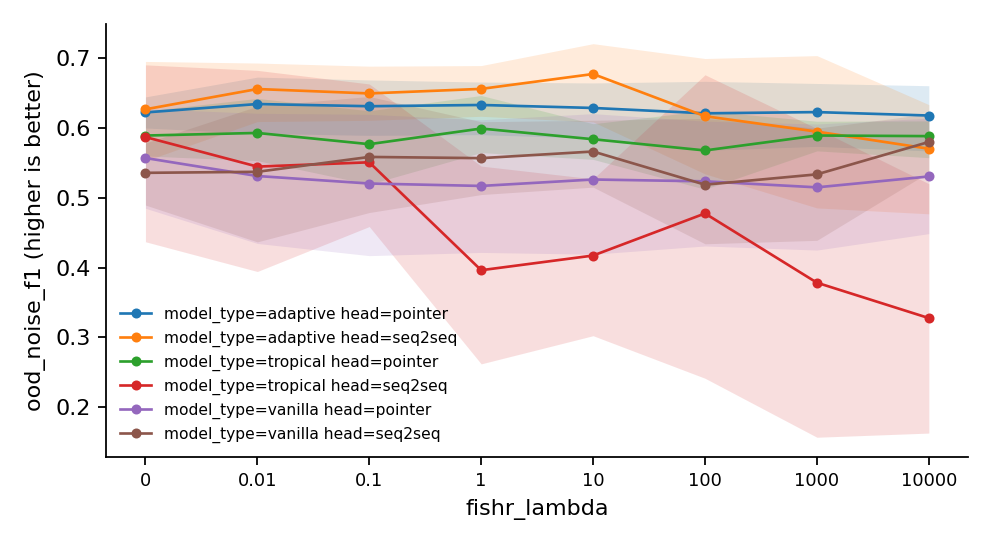
\includegraphics[width=\textwidth]{metric_ood_noise_f1.png}
\caption{\texttt{ood\_noise\_f1} against \texttt{fishr\_lambda}: the mean over seeds with a 95\% bootstrap CI, one line per combination of the other factors.}
\label{fig:ood_noise_f1}
\end{figure}

{\small
\begin{longtable}{lllrlrrr}
\caption{\texttt{ood\_noise\_f1} per cell: mean, 95\% bootstrap CI, SD, seeds, diverged runs.}\label{tab:summary-ood_noise_f1}\\
\toprule
\texttt{model\_type} & \texttt{head} & \texttt{fishr\_lambda} & mean & 95\% CI & SD & $n$ & div.\\
\midrule
\endhead
adaptive & pointer & 0 & 0.6224 & [0.6, 0.645] & 0.0297 & 5 & 0\\
adaptive & pointer & 0.01 & 0.6344 & [0.592, 0.673] & 0.0521 & 5 & 0\\
adaptive & pointer & 0.1 & 0.6313 & [0.589, 0.669] & 0.0526 & 5 & 0\\
adaptive & pointer & 1 & 0.6331 & [0.591, 0.666] & 0.0476 & 5 & 0\\
adaptive & pointer & 10 & 0.6288 & [0.586, 0.665] & 0.0508 & 5 & 0\\
adaptive & pointer & 100 & 0.6211 & [0.568, 0.667] & 0.0638 & 5 & 0\\
adaptive & pointer & 1000 & 0.6229 & [0.574, 0.664] & 0.0595 & 5 & 0\\
adaptive & pointer & 1e+04 & 0.618 & [0.567, 0.661] & 0.0641 & 5 & 0\\
adaptive & seq2seq & 0 & 0.6269 & [0.553, 0.696] & 0.096 & 5 & 0\\
adaptive & seq2seq & 0.01 & 0.656 & [0.609, 0.693] & 0.0544 & 5 & 0\\
adaptive & seq2seq & 0.1 & 0.6497 & [0.611, 0.689] & 0.0516 & 5 & 0\\
adaptive & seq2seq & 1 & 0.6562 & [0.617, 0.69] & 0.0466 & 5 & 0\\
adaptive & seq2seq & 10 & 0.6775 & [0.609, 0.721] & 0.0769 & 5 & 0\\
adaptive & seq2seq & 100 & 0.617 & [0.534, 0.7] & 0.107 & 5 & 0\\
adaptive & seq2seq & 1000 & 0.5949 & [0.486, 0.704] & 0.137 & 5 & 0\\
adaptive & seq2seq & 1e+04 & 0.5704 & [0.477, 0.634] & 0.104 & 5 & 0\\
tropical & pointer & 0 & 0.5893 & [0.56, 0.624] & 0.0424 & 5 & 0\\
tropical & pointer & 0.01 & 0.593 & [0.553, 0.643] & 0.0567 & 5 & 0\\
tropical & pointer & 0.1 & 0.5769 & [0.519, 0.625] & 0.067 & 5 & 0\\
tropical & pointer & 1 & 0.5993 & [0.565, 0.647] & 0.0546 & 5 & 0\\
tropical & pointer & 10 & 0.584 & [0.555, 0.606] & 0.0335 & 5 & 0\\
tropical & pointer & 100 & 0.5679 & [0.512, 0.625] & 0.0766 & 5 & 0\\
tropical & pointer & 1000 & 0.5893 & [0.567, 0.61] & 0.0286 & 5 & 0\\
tropical & pointer & 1e+04 & 0.5884 & [0.558, 0.61] & 0.0338 & 5 & 0\\
tropical & seq2seq & 0 & 0.5871 & [0.437, 0.691] & 0.167 & 5 & 0\\
tropical & seq2seq & 0.01 & 0.5447 & [0.394, 0.683] & 0.195 & 5 & 0\\
tropical & seq2seq & 0.1 & 0.5509 & [0.459, 0.663] & 0.133 & 5 & 0\\
tropical & seq2seq & 1 & 0.3962 & [0.262, 0.546] & 0.179 & 5 & 0\\
tropical & seq2seq & 10 & 0.4172 & [0.302, 0.527] & 0.153 & 5 & 0\\
tropical & seq2seq & 100 & 0.4776 & [0.241, 0.676] & 0.278 & 5 & 0\\
tropical & seq2seq & 1000 & 0.3783 & [0.157, 0.599] & 0.279 & 5 & 0\\
tropical & seq2seq & 1e+04 & 0.3276 & [0.163, 0.52] & 0.23 & 5 & 0\\
vanilla & pointer & 0 & 0.5571 & [0.485, 0.628] & 0.0875 & 5 & 0\\
vanilla & pointer & 0.01 & 0.5313 & [0.435, 0.621] & 0.121 & 5 & 0\\
vanilla & pointer & 0.1 & 0.5205 & [0.417, 0.62] & 0.128 & 5 & 0\\
vanilla & pointer & 1 & 0.517 & [0.422, 0.612] & 0.127 & 5 & 0\\
vanilla & pointer & 10 & 0.5263 & [0.419, 0.621] & 0.127 & 5 & 0\\
vanilla & pointer & 100 & 0.5236 & [0.431, 0.61] & 0.118 & 5 & 0\\
vanilla & pointer & 1000 & 0.515 & [0.425, 0.606] & 0.121 & 5 & 0\\
vanilla & pointer & 1e+04 & 0.5306 & [0.449, 0.614] & 0.107 & 5 & 0\\
vanilla & seq2seq & 0 & 0.5358 & [0.49, 0.579] & 0.0569 & 5 & 0\\
vanilla & seq2seq & 0.01 & 0.5373 & [0.437, 0.631] & 0.132 & 5 & 0\\
vanilla & seq2seq & 0.1 & 0.5586 & [0.479, 0.645] & 0.11 & 5 & 0\\
vanilla & seq2seq & 1 & 0.5569 & [0.505, 0.609] & 0.0687 & 5 & 0\\
vanilla & seq2seq & 10 & 0.5664 & [0.515, 0.611] & 0.0617 & 5 & 0\\
vanilla & seq2seq & 100 & 0.5188 & [0.434, 0.614] & 0.115 & 5 & 0\\
vanilla & seq2seq & 1000 & 0.5336 & [0.439, 0.6] & 0.106 & 5 & 0\\
vanilla & seq2seq & 1e+04 & 0.5801 & [0.537, 0.62] & 0.0549 & 5 & 0\\
\bottomrule
\end{longtable}
}

{\small
\begin{longtable}{lllrrrl}
\caption{\texttt{ood\_noise\_f1}: each level of \texttt{fishr\_lambda} against its control (0), within each combination of the other factors. parametric: Dunnett vs control.}\label{tab:control-ood_noise_f1}\\
\toprule
\texttt{model\_type} & \texttt{head} & \texttt{fishr\_lambda} & difference & 95\% CI & $p$ & \\
\midrule
\endhead
adaptive & pointer & 0.01 & 0.01205 & [-0.0815, 0.106] & 0.9994 & \\
adaptive & pointer & 0.1 & 0.008907 & [-0.0846, 0.102] & 0.9999 & \\
adaptive & pointer & 1 & 0.0107 & [-0.0828, 0.104] & 0.9997 & \\
adaptive & pointer & 10 & 0.006423 & [-0.0871, 0.0999] & 1.0000 & \\
adaptive & pointer & 100 & -0.001268 & [-0.0948, 0.0923] & 1.0000 & \\
adaptive & pointer & 1000 & $4.859\times10^{-4}$ & [-0.093, 0.094] & 1.0000 & \\
adaptive & pointer & 1e+04 & -0.00442 & [-0.0979, 0.0891] & 1.0000 & \\
adaptive & seq2seq & 0.01 & 0.02907 & [-0.127, 0.185] & 0.9946 & \\
adaptive & seq2seq & 0.1 & 0.02276 & [-0.134, 0.179] & 0.9988 & \\
adaptive & seq2seq & 1 & 0.02927 & [-0.127, 0.186] & 0.9943 & \\
adaptive & seq2seq & 10 & 0.0506 & [-0.106, 0.207] & 0.9070 & \\
adaptive & seq2seq & 100 & -0.009893 & [-0.166, 0.146] & 1.0000 & \\
adaptive & seq2seq & 1000 & -0.03199 & [-0.188, 0.124] & 0.9906 & \\
adaptive & seq2seq & 1e+04 & -0.05653 & [-0.213, 0.0997] & 0.8550 & \\
tropical & pointer & 0.01 & 0.003727 & [-0.0867, 0.0941] & 1.0000 & \\
tropical & pointer & 0.1 & -0.01237 & [-0.103, 0.078] & 0.9992 & \\
tropical & pointer & 1 & 0.01006 & [-0.0803, 0.1] & 0.9998 & \\
tropical & pointer & 10 & -0.00529 & [-0.0957, 0.0851] & 1.0000 & \\
tropical & pointer & 100 & -0.02136 & [-0.112, 0.069] & 0.9793 & \\
tropical & pointer & 1000 & $5.105\times10^{-5}$ & [-0.0903, 0.0904] & 1.0000 & \\
tropical & pointer & 1e+04 & $-8.351\times10^{-4}$ & [-0.0912, 0.0896] & 1.0000 & \\
tropical & seq2seq & 0.01 & -0.04238 & [-0.406, 0.321] & 0.9997 & \\
tropical & seq2seq & 0.1 & -0.0362 & [-0.4, 0.328] & 0.9999 & \\
tropical & seq2seq & 1 & -0.1909 & [-0.555, 0.173] & 0.5531 & \\
tropical & seq2seq & 10 & -0.1699 & [-0.534, 0.194] & 0.6660 & \\
tropical & seq2seq & 100 & -0.1095 & [-0.473, 0.254] & 0.9323 & \\
tropical & seq2seq & 1000 & -0.2088 & [-0.573, 0.155] & 0.4614 & \\
tropical & seq2seq & 1e+04 & -0.2595 & [-0.623, 0.104] & 0.2501 & \\
vanilla & pointer & 0.01 & -0.02581 & [-0.232, 0.18] & 0.9995 & \\
vanilla & pointer & 0.1 & -0.03657 & [-0.242, 0.169] & 0.9959 & \\
vanilla & pointer & 1 & -0.04004 & [-0.246, 0.166] & 0.9929 & \\
vanilla & pointer & 10 & -0.03082 & [-0.237, 0.175] & 0.9985 & \\
vanilla & pointer & 100 & -0.03344 & [-0.239, 0.172] & 0.9976 & \\
vanilla & pointer & 1000 & -0.04206 & [-0.248, 0.164] & 0.9906 & \\
vanilla & pointer & 1e+04 & -0.02648 & [-0.232, 0.179] & 0.9994 & \\
vanilla & seq2seq & 0.01 & 0.001473 & [-0.161, 0.164] & 1.0000 & \\
vanilla & seq2seq & 0.1 & 0.0228 & [-0.139, 0.185] & 0.9990 & \\
vanilla & seq2seq & 1 & 0.02106 & [-0.141, 0.183] & 0.9994 & \\
vanilla & seq2seq & 10 & 0.03056 & [-0.132, 0.193] & 0.9941 & \\
vanilla & seq2seq & 100 & -0.01698 & [-0.179, 0.145] & 0.9999 & \\
vanilla & seq2seq & 1000 & -0.002177 & [-0.164, 0.16] & 1.0000 & \\
vanilla & seq2seq & 1e+04 & 0.04425 & [-0.118, 0.206] & 0.9573 & \\
\bottomrule
\end{longtable}
}

{\small
\begin{longtable}{llrrrrr}
\caption{\texttt{ood\_noise\_f1} against log10 \texttt{fishr\_lambda}: parametric: OLS slope t-test, seed-bootstrap CI, with the Jonckheere--Terpstra ordered-trend $\tau$ and $p$.}\label{tab:trend-ood_noise_f1}\\
\toprule
\texttt{model\_type} & \texttt{head} & estimate & 95\% CI & $p$ & JT $\tau$ & JT $p$\\
\midrule
\endhead
adaptive & pointer & -0.002793 & [-0.00538, $-7.45\times10^{-4}$] & 0.5274 & -0.101 & 0.4545\\
adaptive & seq2seq & -0.01448 & [-0.0374, 0.00618] & 0.0502 & -0.128 & 0.3531\\
tropical & pointer & $-7.237\times10^{-4}$ & [-0.00816, 0.00661] & 0.8644 & 0.0476 & 0.7425\\
tropical & seq2seq & -0.03269 & [-0.0625, -0.00101] & 0.0641 & -0.211 & 0.1134\\
vanilla & pointer & $-2.281\times10^{-4}$ & [-0.00453, 0.00407] & 0.9809 & -0.0324 & 0.8248\\
vanilla & seq2seq & 0.001441 & [-0.0067, 0.00915] & 0.8533 & 0.04 & 0.7724\\
\bottomrule
\end{longtable}
}

{\small
\begin{longtable}{lrrrl}
\caption{\texttt{ood\_noise\_f1}: paired contrasts by seed, Holm-corrected across the cells. parametric: paired t-test by seed, Holm.}\label{tab:paired-ood_noise_f1}\\
\toprule
contrast (within) & difference & 95\% CI & $p$ & \\
\midrule
\endhead
\stackcell{model\_type: tropical - vanilla\\\footnotesize head=pointer fishr\_lambda=0 } & 0.0322 & [-0.0771, 0.142] & 1.0000 & \\
\stackcell{model\_type: tropical - vanilla\\\footnotesize head=pointer fishr\_lambda=0.01 } & 0.06174 & [-0.14, 0.263] & 1.0000 & \\
\stackcell{model\_type: tropical - vanilla\\\footnotesize head=pointer fishr\_lambda=0.1 } & 0.0564 & [-0.14, 0.253] & 1.0000 & \\
\stackcell{model\_type: tropical - vanilla\\\footnotesize head=pointer fishr\_lambda=1 } & 0.0823 & [-0.114, 0.278] & 1.0000 & \\
\stackcell{model\_type: tropical - vanilla\\\footnotesize head=pointer fishr\_lambda=10 } & 0.05773 & [-0.102, 0.217] & 1.0000 & \\
\stackcell{model\_type: tropical - vanilla\\\footnotesize head=pointer fishr\_lambda=100 } & 0.04428 & [-0.125, 0.214] & 1.0000 & \\
\stackcell{model\_type: tropical - vanilla\\\footnotesize head=pointer fishr\_lambda=1000 } & 0.07432 & [-0.0722, 0.221] & 1.0000 & \\
\stackcell{model\_type: tropical - vanilla\\\footnotesize head=pointer fishr\_lambda=1e+04 } & 0.05784 & [-0.0898, 0.206] & 1.0000 & \\
\stackcell{model\_type: tropical - vanilla\\\footnotesize head=seq2seq fishr\_lambda=0 } & 0.05131 & [-0.0941, 0.197] & 1.0000 & \\
\stackcell{model\_type: tropical - vanilla\\\footnotesize head=seq2seq fishr\_lambda=0.01 } & 0.00745 & [-0.183, 0.198] & 1.0000 & \\
\stackcell{model\_type: tropical - vanilla\\\footnotesize head=seq2seq fishr\_lambda=0.1 } & -0.007687 & [-0.153, 0.137] & 1.0000 & \\
\stackcell{model\_type: tropical - vanilla\\\footnotesize head=seq2seq fishr\_lambda=1 } & -0.1607 & [-0.386, 0.0648] & 1.0000 & \\
\stackcell{model\_type: tropical - vanilla\\\footnotesize head=seq2seq fishr\_lambda=10 } & -0.1491 & [-0.313, 0.0143] & 1.0000 & \\
\stackcell{model\_type: tropical - vanilla\\\footnotesize head=seq2seq fishr\_lambda=100 } & -0.04124 & [-0.291, 0.209] & 1.0000 & \\
\stackcell{model\_type: tropical - vanilla\\\footnotesize head=seq2seq fishr\_lambda=1000 } & -0.1553 & [-0.441, 0.131] & 1.0000 & \\
\stackcell{model\_type: tropical - vanilla\\\footnotesize head=seq2seq fishr\_lambda=1e+04 } & -0.2525 & [-0.533, 0.0283] & 1.0000 & \\
\stackcell{model\_type: adaptive - vanilla\\\footnotesize head=pointer fishr\_lambda=0 } & 0.06533 & [-0.0393, 0.17] & 1.0000 & \\
\stackcell{model\_type: adaptive - vanilla\\\footnotesize head=pointer fishr\_lambda=0.01 } & 0.1032 & [-0.0473, 0.254] & 1.0000 & \\
\stackcell{model\_type: adaptive - vanilla\\\footnotesize head=pointer fishr\_lambda=0.1 } & 0.1108 & [-0.0382, 0.26] & 1.0000 & \\
\stackcell{model\_type: adaptive - vanilla\\\footnotesize head=pointer fishr\_lambda=1 } & 0.1161 & [-0.0394, 0.272] & 1.0000 & \\
\stackcell{model\_type: adaptive - vanilla\\\footnotesize head=pointer fishr\_lambda=10 } & 0.1026 & [-0.0582, 0.263] & 1.0000 & \\
\stackcell{model\_type: adaptive - vanilla\\\footnotesize head=pointer fishr\_lambda=100 } & 0.0975 & [-0.037, 0.232] & 1.0000 & \\
\stackcell{model\_type: adaptive - vanilla\\\footnotesize head=pointer fishr\_lambda=1000 } & 0.1079 & [-0.042, 0.258] & 1.0000 & \\
\stackcell{model\_type: adaptive - vanilla\\\footnotesize head=pointer fishr\_lambda=1e+04 } & 0.08738 & [-0.0668, 0.242] & 1.0000 & \\
\stackcell{model\_type: adaptive - vanilla\\\footnotesize head=seq2seq fishr\_lambda=0 } & 0.09108 & [-0.0327, 0.215] & 1.0000 & \\
\stackcell{model\_type: adaptive - vanilla\\\footnotesize head=seq2seq fishr\_lambda=0.01 } & 0.1187 & [-0.0687, 0.306] & 1.0000 & \\
\stackcell{model\_type: adaptive - vanilla\\\footnotesize head=seq2seq fishr\_lambda=0.1 } & 0.09104 & [-0.057, 0.239] & 1.0000 & \\
\stackcell{model\_type: adaptive - vanilla\\\footnotesize head=seq2seq fishr\_lambda=1 } & 0.09929 & [-0.0162, 0.215] & 1.0000 & \\
\stackcell{model\_type: adaptive - vanilla\\\footnotesize head=seq2seq fishr\_lambda=10 } & 0.1111 & [0.0526, 0.17] & 0.0929 & \\
\stackcell{model\_type: adaptive - vanilla\\\footnotesize head=seq2seq fishr\_lambda=100 } & 0.09817 & [0.0548, 0.142] & 0.0526 & \\
\stackcell{model\_type: adaptive - vanilla\\\footnotesize head=seq2seq fishr\_lambda=1000 } & 0.06127 & [-0.0584, 0.181] & 1.0000 & \\
\stackcell{model\_type: adaptive - vanilla\\\footnotesize head=seq2seq fishr\_lambda=1e+04 } & -0.009702 & [-0.0942, 0.0748] & 1.0000 & \\
\stackcell{head: pointer - seq2seq\\\footnotesize model\_type=adaptive fishr\_lambda=0 } & -0.004495 & [-0.137, 0.128] & 1.0000 & \\
\stackcell{head: pointer - seq2seq\\\footnotesize model\_type=adaptive fishr\_lambda=0.01 } & -0.02152 & [-0.0351, -0.0079] & 0.2719 & \\
\stackcell{head: pointer - seq2seq\\\footnotesize model\_type=adaptive fishr\_lambda=0.1 } & -0.01835 & [-0.0498, 0.0131] & 1.0000 & \\
\stackcell{head: pointer - seq2seq\\\footnotesize model\_type=adaptive fishr\_lambda=1 } & -0.02306 & [-0.0346, -0.0115] & 0.1240 & \\
\stackcell{head: pointer - seq2seq\\\footnotesize model\_type=adaptive fishr\_lambda=10 } & -0.04867 & [-0.157, 0.0594] & 1.0000 & \\
\stackcell{head: pointer - seq2seq\\\footnotesize model\_type=adaptive fishr\_lambda=100 } & 0.00413 & [-0.165, 0.173] & 1.0000 & \\
\stackcell{head: pointer - seq2seq\\\footnotesize model\_type=adaptive fishr\_lambda=1000 } & 0.02798 & [-0.165, 0.221] & 1.0000 & \\
\stackcell{head: pointer - seq2seq\\\footnotesize model\_type=adaptive fishr\_lambda=1e+04 } & 0.04761 & [-0.112, 0.208] & 1.0000 & \\
\stackcell{head: pointer - seq2seq\\\footnotesize model\_type=tropical fishr\_lambda=0 } & 0.002152 & [-0.201, 0.205] & 1.0000 & \\
\stackcell{head: pointer - seq2seq\\\footnotesize model\_type=tropical fishr\_lambda=0.01 } & 0.04826 & [-0.225, 0.321] & 1.0000 & \\
\stackcell{head: pointer - seq2seq\\\footnotesize model\_type=tropical fishr\_lambda=0.1 } & 0.02598 & [-0.211, 0.263] & 1.0000 & \\
\stackcell{head: pointer - seq2seq\\\footnotesize model\_type=tropical fishr\_lambda=1 } & 0.2031 & [-0.0692, 0.475] & 1.0000 & \\
\stackcell{head: pointer - seq2seq\\\footnotesize model\_type=tropical fishr\_lambda=10 } & 0.1667 & [-0.05, 0.383] & 1.0000 & \\
\stackcell{head: pointer - seq2seq\\\footnotesize model\_type=tropical fishr\_lambda=100 } & 0.09032 & [-0.334, 0.515] & 1.0000 & \\
\stackcell{head: pointer - seq2seq\\\footnotesize model\_type=tropical fishr\_lambda=1000 } & 0.211 & [-0.142, 0.564] & 1.0000 & \\
\stackcell{head: pointer - seq2seq\\\footnotesize model\_type=tropical fishr\_lambda=1e+04 } & 0.2609 & [-0.0514, 0.573] & 1.0000 & \\
\stackcell{head: pointer - seq2seq\\\footnotesize model\_type=vanilla fishr\_lambda=0 } & 0.02126 & [-0.0559, 0.0984] & 1.0000 & \\
\stackcell{head: pointer - seq2seq\\\footnotesize model\_type=vanilla fishr\_lambda=0.01 } & -0.006029 & [-0.161, 0.149] & 1.0000 & \\
\stackcell{head: pointer - seq2seq\\\footnotesize model\_type=vanilla fishr\_lambda=0.1 } & -0.03811 & [-0.209, 0.133] & 1.0000 & \\
\stackcell{head: pointer - seq2seq\\\footnotesize model\_type=vanilla fishr\_lambda=1 } & -0.03984 & [-0.234, 0.154] & 1.0000 & \\
\stackcell{head: pointer - seq2seq\\\footnotesize model\_type=vanilla fishr\_lambda=10 } & -0.04012 & [-0.222, 0.142] & 1.0000 & \\
\stackcell{head: pointer - seq2seq\\\footnotesize model\_type=vanilla fishr\_lambda=100 } & 0.004803 & [-0.136, 0.145] & 1.0000 & \\
\stackcell{head: pointer - seq2seq\\\footnotesize model\_type=vanilla fishr\_lambda=1000 } & -0.01863 & [-0.156, 0.119] & 1.0000 & \\
\stackcell{head: pointer - seq2seq\\\footnotesize model\_type=vanilla fishr\_lambda=1e+04 } & -0.04947 & [-0.18, 0.0813] & 1.0000 & \\
\bottomrule
\end{longtable}
}

\subsection{\texttt{ood\_noise\_exact}}
\begin{figure}[tbp]
\centering
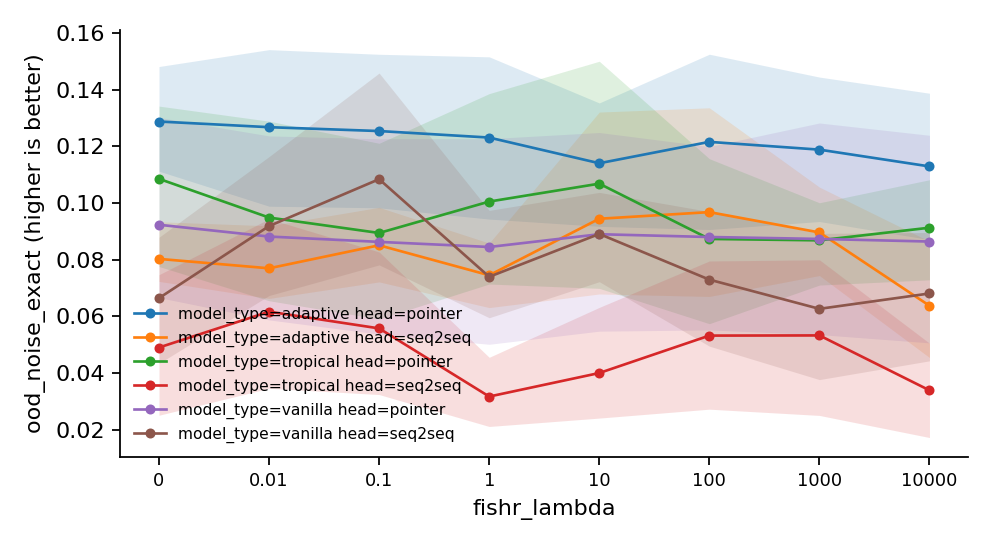
\includegraphics[width=\textwidth]{metric_ood_noise_exact.png}
\caption{\texttt{ood\_noise\_exact} against \texttt{fishr\_lambda}: the mean over seeds with a 95\% bootstrap CI, one line per combination of the other factors.}
\label{fig:ood_noise_exact}
\end{figure}

{\small
\begin{longtable}{lllrlrrr}
\caption{\texttt{ood\_noise\_exact} per cell: mean, 95\% bootstrap CI, SD, seeds, diverged runs.}\label{tab:summary-ood_noise_exact}\\
\toprule
\texttt{model\_type} & \texttt{head} & \texttt{fishr\_lambda} & mean & 95\% CI & SD & $n$ & div.\\
\midrule
\endhead
adaptive & pointer & 0 & 0.1287 & [0.111, 0.148] & 0.0243 & 5 & 0\\
adaptive & pointer & 0.01 & 0.1267 & [0.0988, 0.154] & 0.0359 & 5 & 0\\
adaptive & pointer & 0.1 & 0.1254 & [0.0983, 0.152] & 0.0356 & 5 & 0\\
adaptive & pointer & 1 & 0.1231 & [0.0943, 0.152] & 0.038 & 5 & 0\\
adaptive & pointer & 10 & 0.114 & [0.0917, 0.135] & 0.0279 & 5 & 0\\
adaptive & pointer & 100 & 0.1215 & [0.0906, 0.152] & 0.0398 & 5 & 0\\
adaptive & pointer & 1000 & 0.1188 & [0.0934, 0.144] & 0.033 & 5 & 0\\
adaptive & pointer & 1e+04 & 0.1129 & [0.0871, 0.139] & 0.036 & 5 & 0\\
adaptive & seq2seq & 0 & 0.08026 & [0.0723, 0.0934] & 0.0147 & 5 & 0\\
adaptive & seq2seq & 0.01 & 0.07694 & [0.0663, 0.0919] & 0.0176 & 5 & 0\\
adaptive & seq2seq & 0.1 & 0.08506 & [0.0721, 0.0984] & 0.0174 & 5 & 0\\
adaptive & seq2seq & 1 & 0.07448 & [0.0631, 0.0858] & 0.0143 & 5 & 0\\
adaptive & seq2seq & 10 & 0.09442 & [0.0679, 0.132] & 0.0431 & 5 & 0\\
adaptive & seq2seq & 100 & 0.09676 & [0.067, 0.134] & 0.0448 & 5 & 0\\
adaptive & seq2seq & 1000 & 0.08958 & [0.0744, 0.106] & 0.0204 & 5 & 0\\
adaptive & seq2seq & 1e+04 & 0.06374 & [0.0455, 0.0865] & 0.0276 & 5 & 0\\
tropical & pointer & 0 & 0.1085 & [0.0776, 0.134] & 0.0358 & 5 & 0\\
tropical & pointer & 0.01 & 0.09484 & [0.0655, 0.129] & 0.0408 & 5 & 0\\
tropical & pointer & 0.1 & 0.0894 & [0.0591, 0.121] & 0.0394 & 5 & 0\\
tropical & pointer & 1 & 0.1005 & [0.0714, 0.139] & 0.0435 & 5 & 0\\
tropical & pointer & 10 & 0.1068 & [0.0699, 0.15] & 0.0496 & 5 & 0\\
tropical & pointer & 100 & 0.0873 & [0.0574, 0.116] & 0.0382 & 5 & 0\\
tropical & pointer & 1000 & 0.0868 & [0.071, 0.1] & 0.019 & 5 & 0\\
tropical & pointer & 1e+04 & 0.09126 & [0.0729, 0.108] & 0.0234 & 5 & 0\\
tropical & seq2seq & 0 & 0.049 & [0.0251, 0.0747] & 0.0332 & 5 & 0\\
tropical & seq2seq & 0.01 & 0.06164 & [0.0346, 0.0944] & 0.0385 & 5 & 0\\
tropical & seq2seq & 0.1 & 0.05574 & [0.0324, 0.0827] & 0.0325 & 5 & 0\\
tropical & seq2seq & 1 & 0.0317 & [0.0211, 0.0455] & 0.0163 & 5 & 0\\
tropical & seq2seq & 10 & 0.04 & [0.0241, 0.0631] & 0.0254 & 5 & 0\\
tropical & seq2seq & 100 & 0.0532 & [0.0272, 0.0795] & 0.0338 & 5 & 0\\
tropical & seq2seq & 1000 & 0.05326 & [0.025, 0.0799] & 0.0356 & 5 & 0\\
tropical & seq2seq & 1e+04 & 0.0339 & [0.0172, 0.0505] & 0.0217 & 5 & 0\\
vanilla & pointer & 0 & 0.0923 & [0.0666, 0.13] & 0.0429 & 5 & 0\\
vanilla & pointer & 0.01 & 0.08814 & [0.0587, 0.124] & 0.0412 & 5 & 0\\
vanilla & pointer & 0.1 & 0.08626 & [0.0537, 0.123] & 0.0455 & 5 & 0\\
vanilla & pointer & 1 & 0.08446 & [0.0501, 0.123] & 0.0469 & 5 & 0\\
vanilla & pointer & 10 & 0.08896 & [0.0548, 0.125] & 0.0463 & 5 & 0\\
vanilla & pointer & 100 & 0.08798 & [0.0552, 0.12] & 0.0426 & 5 & 0\\
vanilla & pointer & 1000 & 0.0873 & [0.0536, 0.128] & 0.0475 & 5 & 0\\
vanilla & pointer & 1e+04 & 0.08638 & [0.0506, 0.124] & 0.0481 & 5 & 0\\
vanilla & seq2seq & 0 & 0.06642 & [0.0434, 0.0879] & 0.029 & 5 & 0\\
vanilla & seq2seq & 0.01 & 0.09184 & [0.0673, 0.116] & 0.0328 & 5 & 0\\
vanilla & seq2seq & 0.1 & 0.1084 & [0.0781, 0.146] & 0.0463 & 5 & 0\\
vanilla & seq2seq & 1 & 0.07394 & [0.0595, 0.0974] & 0.0259 & 5 & 0\\
vanilla & seq2seq & 10 & 0.08906 & [0.0722, 0.104] & 0.0211 & 5 & 0\\
vanilla & seq2seq & 100 & 0.07294 & [0.0495, 0.097] & 0.0307 & 5 & 0\\
vanilla & seq2seq & 1000 & 0.06264 & [0.0377, 0.0893] & 0.0326 & 5 & 0\\
vanilla & seq2seq & 1e+04 & 0.06806 & [0.0443, 0.0896] & 0.0297 & 5 & 0\\
\bottomrule
\end{longtable}
}

{\small
\begin{longtable}{lllrrrl}
\caption{\texttt{ood\_noise\_exact}: each level of \texttt{fishr\_lambda} against its control (0), within each combination of the other factors. parametric: Dunnett vs control.}\label{tab:control-ood_noise_exact}\\
\toprule
\texttt{model\_type} & \texttt{head} & \texttt{fishr\_lambda} & difference & 95\% CI & $p$ & \\
\midrule
\endhead
adaptive & pointer & 0.01 & -0.002 & [-0.0617, 0.0577] & 1.0000 & \\
adaptive & pointer & 0.1 & -0.00336 & [-0.063, 0.0563] & 1.0000 & \\
adaptive & pointer & 1 & -0.00566 & [-0.0653, 0.054] & 0.9999 & \\
adaptive & pointer & 10 & -0.01472 & [-0.0744, 0.045] & 0.9742 & \\
adaptive & pointer & 100 & -0.00718 & [-0.0669, 0.0525] & 0.9996 & \\
adaptive & pointer & 1000 & -0.00992 & [-0.0696, 0.0498] & 0.9972 & \\
adaptive & pointer & 1e+04 & -0.01584 & [-0.0755, 0.0438] & 0.9626 & \\
adaptive & seq2seq & 0.01 & -0.00332 & [-0.0514, 0.0448] & 1.0000 & \\
adaptive & seq2seq & 0.1 & 0.0048 & [-0.0433, 0.0529] & 0.9999 & \\
adaptive & seq2seq & 1 & -0.00578 & [-0.0539, 0.0423] & 0.9996 & \\
adaptive & seq2seq & 10 & 0.01416 & [-0.034, 0.0623] & 0.9390 & \\
adaptive & seq2seq & 100 & 0.0165 & [-0.0316, 0.0646] & 0.8822 & \\
adaptive & seq2seq & 1000 & 0.00932 & [-0.0388, 0.0574] & 0.9931 & \\
adaptive & seq2seq & 1e+04 & -0.01652 & [-0.0646, 0.0316] & 0.8818 & \\
tropical & pointer & 0.01 & -0.01366 & [-0.0791, 0.0518] & 0.9895 & \\
tropical & pointer & 0.1 & -0.0191 & [-0.0845, 0.0463] & 0.9412 & \\
tropical & pointer & 1 & -0.00802 & [-0.0734, 0.0574] & 0.9996 & \\
tropical & pointer & 10 & -0.0017 & [-0.0671, 0.0637] & 1.0000 & \\
tropical & pointer & 100 & -0.0212 & [-0.0866, 0.0442] & 0.9067 & \\
tropical & pointer & 1000 & -0.0217 & [-0.0871, 0.0437] & 0.8972 & \\
tropical & pointer & 1e+04 & -0.01724 & [-0.0827, 0.0482] & 0.9640 & \\
tropical & seq2seq & 0.01 & 0.01264 & [-0.0406, 0.0659] & 0.9788 & \\
tropical & seq2seq & 0.1 & 0.00674 & [-0.0465, 0.06] & 0.9995 & \\
tropical & seq2seq & 1 & -0.0173 & [-0.0705, 0.0359] & 0.9056 & \\
tropical & seq2seq & 10 & -0.009 & [-0.0622, 0.0442] & 0.9969 & \\
tropical & seq2seq & 100 & 0.0042 & [-0.049, 0.0574] & 1.0000 & \\
tropical & seq2seq & 1000 & 0.00426 & [-0.049, 0.0575] & 1.0000 & \\
tropical & seq2seq & 1e+04 & -0.0151 & [-0.0683, 0.0381] & 0.9486 & \\
vanilla & pointer & 0.01 & -0.00416 & [-0.0831, 0.0748] & 1.0000 & \\
vanilla & pointer & 0.1 & -0.00604 & [-0.085, 0.0729] & 1.0000 & \\
vanilla & pointer & 1 & -0.00784 & [-0.0868, 0.0711] & 0.9999 & \\
vanilla & pointer & 10 & -0.00334 & [-0.0823, 0.0756] & 1.0000 & \\
vanilla & pointer & 100 & -0.00432 & [-0.0833, 0.0746] & 1.0000 & \\
vanilla & pointer & 1000 & -0.005 & [-0.0839, 0.0739] & 1.0000 & \\
vanilla & pointer & 1e+04 & -0.00592 & [-0.0849, 0.073] & 1.0000 & \\
vanilla & seq2seq & 0.01 & 0.02542 & [-0.03, 0.0809] & 0.6827 & \\
vanilla & seq2seq & 0.1 & 0.04196 & [-0.0135, 0.0974] & 0.2015 & \\
vanilla & seq2seq & 1 & 0.00752 & [-0.0479, 0.063] & 0.9992 & \\
vanilla & seq2seq & 10 & 0.02264 & [-0.0328, 0.0781] & 0.7772 & \\
vanilla & seq2seq & 100 & 0.00652 & [-0.0489, 0.062] & 0.9997 & \\
vanilla & seq2seq & 1000 & -0.00378 & [-0.0592, 0.0517] & 1.0000 & \\
vanilla & seq2seq & 1e+04 & 0.00164 & [-0.0538, 0.0571] & 1.0000 & \\
\bottomrule
\end{longtable}
}

{\small
\begin{longtable}{llrrrrr}
\caption{\texttt{ood\_noise\_exact} against log10 \texttt{fishr\_lambda}: parametric: OLS slope t-test, seed-bootstrap CI, with the Jonckheere--Terpstra ordered-trend $\tau$ and $p$.}\label{tab:trend-ood_noise_exact}\\
\toprule
\texttt{model\_type} & \texttt{head} & estimate & 95\% CI & $p$ & JT $\tau$ & JT $p$\\
\midrule
\endhead
adaptive & pointer & -0.002006 & [-0.00292, -0.00111] & 0.4732 & -0.0895 & 0.5039\\
adaptive & seq2seq & $-2.957\times10^{-4}$ & [-0.00491, 0.00432] & 0.9045 & -0.0171 & 0.9048\\
tropical & pointer & -0.00104 & [-0.00539, 0.00244] & 0.7301 & -0.0019 & 1.0000\\
tropical & seq2seq & -0.002381 & [-0.00984, 0.00244] & 0.3457 & -0.177 & 0.1886\\
vanilla & pointer & $1.143\times10^{-5}$ & [-0.002, 0.00249] & 0.9974 & -0.0533 & 0.6931\\
vanilla & seq2seq & -0.005851 & [-0.0103, -0.00146] & 0.0328 & -0.23 & 0.0864\\
\bottomrule
\end{longtable}
}

{\small
\begin{longtable}{lrrrl}
\caption{\texttt{ood\_noise\_exact}: paired contrasts by seed, Holm-corrected across the cells. parametric: paired t-test by seed, Holm.}\label{tab:paired-ood_noise_exact}\\
\toprule
contrast (within) & difference & 95\% CI & $p$ & \\
\midrule
\endhead
\stackcell{model\_type: tropical - vanilla\\\footnotesize head=pointer fishr\_lambda=0 } & 0.0162 & [-0.0355, 0.0679] & 1.0000 & \\
\stackcell{model\_type: tropical - vanilla\\\footnotesize head=pointer fishr\_lambda=0.01 } & 0.0067 & [-0.0763, 0.0897] & 1.0000 & \\
\stackcell{model\_type: tropical - vanilla\\\footnotesize head=pointer fishr\_lambda=0.1 } & 0.00314 & [-0.0672, 0.0735] & 1.0000 & \\
\stackcell{model\_type: tropical - vanilla\\\footnotesize head=pointer fishr\_lambda=1 } & 0.01602 & [-0.0602, 0.0922] & 1.0000 & \\
\stackcell{model\_type: tropical - vanilla\\\footnotesize head=pointer fishr\_lambda=10 } & 0.01784 & [-0.0695, 0.105] & 1.0000 & \\
\stackcell{model\_type: tropical - vanilla\\\footnotesize head=pointer fishr\_lambda=100 } & $-6.800\times10^{-4}$ & [-0.0597, 0.0583] & 1.0000 & \\
\stackcell{model\_type: tropical - vanilla\\\footnotesize head=pointer fishr\_lambda=1000 } & $-5.000\times10^{-4}$ & [-0.048, 0.047] & 1.0000 & \\
\stackcell{model\_type: tropical - vanilla\\\footnotesize head=pointer fishr\_lambda=1e+04 } & 0.00488 & [-0.0504, 0.0602] & 1.0000 & \\
\stackcell{model\_type: tropical - vanilla\\\footnotesize head=seq2seq fishr\_lambda=0 } & -0.01742 & [-0.0729, 0.038] & 1.0000 & \\
\stackcell{model\_type: tropical - vanilla\\\footnotesize head=seq2seq fishr\_lambda=0.01 } & -0.0302 & [-0.0783, 0.0179] & 1.0000 & \\
\stackcell{model\_type: tropical - vanilla\\\footnotesize head=seq2seq fishr\_lambda=0.1 } & -0.05264 & [-0.129, 0.0242] & 1.0000 & \\
\stackcell{model\_type: tropical - vanilla\\\footnotesize head=seq2seq fishr\_lambda=1 } & -0.04224 & [-0.0788, -0.00566] & 0.4579 & \\
\stackcell{model\_type: tropical - vanilla\\\footnotesize head=seq2seq fishr\_lambda=10 } & -0.04906 & [-0.0901, -0.00802] & 0.4520 & \\
\stackcell{model\_type: tropical - vanilla\\\footnotesize head=seq2seq fishr\_lambda=100 } & -0.01974 & [-0.036, -0.00344] & 0.4520 & \\
\stackcell{model\_type: tropical - vanilla\\\footnotesize head=seq2seq fishr\_lambda=1000 } & -0.00938 & [-0.0689, 0.0501] & 1.0000 & \\
\stackcell{model\_type: tropical - vanilla\\\footnotesize head=seq2seq fishr\_lambda=1e+04 } & -0.03416 & [-0.0887, 0.0204] & 1.0000 & \\
\stackcell{model\_type: adaptive - vanilla\\\footnotesize head=pointer fishr\_lambda=0 } & 0.03642 & [-0.0201, 0.0929] & 1.0000 & \\
\stackcell{model\_type: adaptive - vanilla\\\footnotesize head=pointer fishr\_lambda=0.01 } & 0.03858 & [-0.0282, 0.105] & 1.0000 & \\
\stackcell{model\_type: adaptive - vanilla\\\footnotesize head=pointer fishr\_lambda=0.1 } & 0.0391 & [-0.0268, 0.105] & 1.0000 & \\
\stackcell{model\_type: adaptive - vanilla\\\footnotesize head=pointer fishr\_lambda=1 } & 0.0386 & [-0.0317, 0.109] & 1.0000 & \\
\stackcell{model\_type: adaptive - vanilla\\\footnotesize head=pointer fishr\_lambda=10 } & 0.02504 & [-0.0474, 0.0975] & 1.0000 & \\
\stackcell{model\_type: adaptive - vanilla\\\footnotesize head=pointer fishr\_lambda=100 } & 0.03356 & [-0.0235, 0.0906] & 1.0000 & \\
\stackcell{model\_type: adaptive - vanilla\\\footnotesize head=pointer fishr\_lambda=1000 } & 0.0315 & [-0.0377, 0.101] & 1.0000 & \\
\stackcell{model\_type: adaptive - vanilla\\\footnotesize head=pointer fishr\_lambda=1e+04 } & 0.0265 & [-0.0504, 0.103] & 1.0000 & \\
\stackcell{model\_type: adaptive - vanilla\\\footnotesize head=seq2seq fishr\_lambda=0 } & 0.01384 & [-0.0311, 0.0588] & 1.0000 & \\
\stackcell{model\_type: adaptive - vanilla\\\footnotesize head=seq2seq fishr\_lambda=0.01 } & -0.0149 & [-0.0401, 0.0103] & 1.0000 & \\
\stackcell{model\_type: adaptive - vanilla\\\footnotesize head=seq2seq fishr\_lambda=0.1 } & -0.02332 & [-0.0714, 0.0248] & 1.0000 & \\
\stackcell{model\_type: adaptive - vanilla\\\footnotesize head=seq2seq fishr\_lambda=1 } & $5.400\times10^{-4}$ & [-0.0278, 0.0289] & 1.0000 & \\
\stackcell{model\_type: adaptive - vanilla\\\footnotesize head=seq2seq fishr\_lambda=10 } & 0.00536 & [-0.0405, 0.0512] & 1.0000 & \\
\stackcell{model\_type: adaptive - vanilla\\\footnotesize head=seq2seq fishr\_lambda=100 } & 0.02382 & [-0.0375, 0.0852] & 1.0000 & \\
\stackcell{model\_type: adaptive - vanilla\\\footnotesize head=seq2seq fishr\_lambda=1000 } & 0.02694 & [-0.012, 0.0659] & 1.0000 & \\
\stackcell{model\_type: adaptive - vanilla\\\footnotesize head=seq2seq fishr\_lambda=1e+04 } & -0.00432 & [-0.0278, 0.0192] & 1.0000 & \\
\stackcell{head: pointer - seq2seq\\\footnotesize model\_type=adaptive fishr\_lambda=0 } & 0.04846 & [0.0141, 0.0828] & 0.3807 & \\
\stackcell{head: pointer - seq2seq\\\footnotesize model\_type=adaptive fishr\_lambda=0.01 } & 0.04978 & [0.016, 0.0835] & 0.3427 & \\
\stackcell{head: pointer - seq2seq\\\footnotesize model\_type=adaptive fishr\_lambda=0.1 } & 0.0403 & [-0.00354, 0.0841] & 1.0000 & \\
\stackcell{head: pointer - seq2seq\\\footnotesize model\_type=adaptive fishr\_lambda=1 } & 0.04858 & [0.0061, 0.0911] & 0.6996 & \\
\stackcell{head: pointer - seq2seq\\\footnotesize model\_type=adaptive fishr\_lambda=10 } & 0.01958 & [-0.0583, 0.0975] & 1.0000 & \\
\stackcell{head: pointer - seq2seq\\\footnotesize model\_type=adaptive fishr\_lambda=100 } & 0.02478 & [-0.0607, 0.11] & 1.0000 & \\
\stackcell{head: pointer - seq2seq\\\footnotesize model\_type=adaptive fishr\_lambda=1000 } & 0.02922 & [-0.013, 0.0715] & 1.0000 & \\
\stackcell{head: pointer - seq2seq\\\footnotesize model\_type=adaptive fishr\_lambda=1e+04 } & 0.04914 & [0.00383, 0.0945] & 0.7378 & \\
\stackcell{head: pointer - seq2seq\\\footnotesize model\_type=tropical fishr\_lambda=0 } & 0.0595 & [0.00496, 0.114] & 0.7378 & \\
\stackcell{head: pointer - seq2seq\\\footnotesize model\_type=tropical fishr\_lambda=0.01 } & 0.0332 & [-0.0593, 0.126] & 1.0000 & \\
\stackcell{head: pointer - seq2seq\\\footnotesize model\_type=tropical fishr\_lambda=0.1 } & 0.03366 & [-0.0533, 0.121] & 1.0000 & \\
\stackcell{head: pointer - seq2seq\\\footnotesize model\_type=tropical fishr\_lambda=1 } & 0.06878 & [0.00886, 0.129] & 0.6996 & \\
\stackcell{head: pointer - seq2seq\\\footnotesize model\_type=tropical fishr\_lambda=10 } & 0.0668 & [-0.0114, 0.145] & 1.0000 & \\
\stackcell{head: pointer - seq2seq\\\footnotesize model\_type=tropical fishr\_lambda=100 } & 0.0341 & [-0.037, 0.105] & 1.0000 & \\
\stackcell{head: pointer - seq2seq\\\footnotesize model\_type=tropical fishr\_lambda=1000 } & 0.03354 & [-0.00504, 0.0721] & 1.0000 & \\
\stackcell{head: pointer - seq2seq\\\footnotesize model\_type=tropical fishr\_lambda=1e+04 } & 0.05736 & [0.0233, 0.0915] & 0.2286 & \\
\stackcell{head: pointer - seq2seq\\\footnotesize model\_type=vanilla fishr\_lambda=0 } & 0.02588 & [-0.0158, 0.0675] & 1.0000 & \\
\stackcell{head: pointer - seq2seq\\\footnotesize model\_type=vanilla fishr\_lambda=0.01 } & -0.0037 & [-0.0719, 0.0645] & 1.0000 & \\
\stackcell{head: pointer - seq2seq\\\footnotesize model\_type=vanilla fishr\_lambda=0.1 } & -0.02212 & [-0.104, 0.0602] & 1.0000 & \\
\stackcell{head: pointer - seq2seq\\\footnotesize model\_type=vanilla fishr\_lambda=1 } & 0.01052 & [-0.0658, 0.0868] & 1.0000 & \\
\stackcell{head: pointer - seq2seq\\\footnotesize model\_type=vanilla fishr\_lambda=10 } & $-1.000\times10^{-4}$ & [-0.0761, 0.0759] & 1.0000 & \\
\stackcell{head: pointer - seq2seq\\\footnotesize model\_type=vanilla fishr\_lambda=100 } & 0.01504 & [-0.0305, 0.0606] & 1.0000 & \\
\stackcell{head: pointer - seq2seq\\\footnotesize model\_type=vanilla fishr\_lambda=1000 } & 0.02466 & [-0.0495, 0.0988] & 1.0000 & \\
\stackcell{head: pointer - seq2seq\\\footnotesize model\_type=vanilla fishr\_lambda=1e+04 } & 0.01832 & [-0.0534, 0.0901] & 1.0000 & \\
\bottomrule
\end{longtable}
}

\subsection{\texttt{id\_f1}}
\begin{figure}[tbp]
\centering
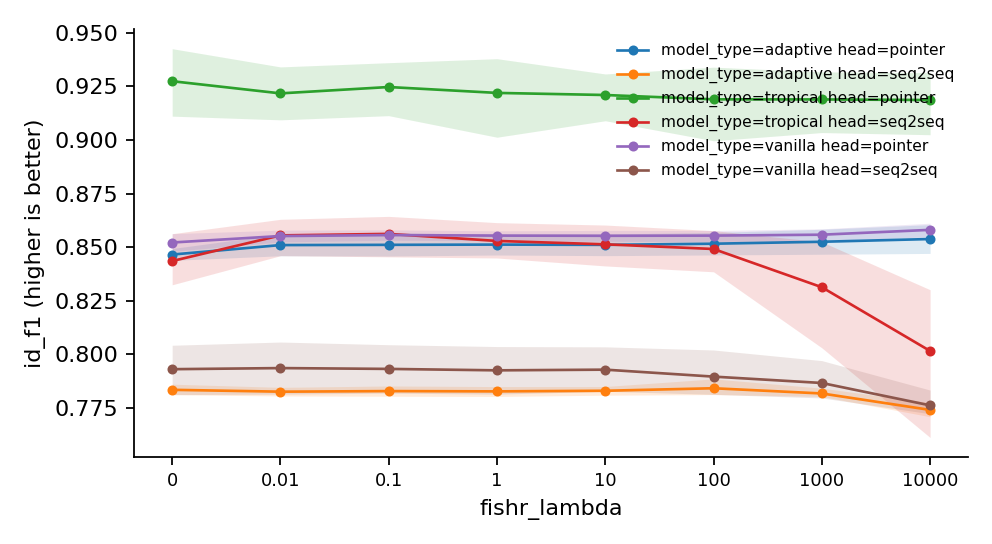
\includegraphics[width=\textwidth]{metric_id_f1.png}
\caption{\texttt{id\_f1} against \texttt{fishr\_lambda}: the mean over seeds with a 95\% bootstrap CI, one line per combination of the other factors.}
\label{fig:id_f1}
\end{figure}

{\small
\begin{longtable}{lllrlrrr}
\caption{\texttt{id\_f1} per cell: mean, 95\% bootstrap CI, SD, seeds, diverged runs.}\label{tab:summary-id_f1}\\
\toprule
\texttt{model\_type} & \texttt{head} & \texttt{fishr\_lambda} & mean & 95\% CI & SD & $n$ & div.\\
\midrule
\endhead
adaptive & pointer & 0 & 0.8466 & [0.844, 0.849] & 0.00361 & 5 & 0\\
adaptive & pointer & 0.01 & 0.851 & [0.846, 0.856] & 0.00681 & 5 & 0\\
adaptive & pointer & 0.1 & 0.8511 & [0.846, 0.857] & 0.00702 & 5 & 0\\
adaptive & pointer & 1 & 0.8512 & [0.846, 0.856] & 0.00651 & 5 & 0\\
adaptive & pointer & 10 & 0.8511 & [0.846, 0.856] & 0.00657 & 5 & 0\\
adaptive & pointer & 100 & 0.8516 & [0.846, 0.857] & 0.00692 & 5 & 0\\
adaptive & pointer & 1000 & 0.8525 & [0.847, 0.858] & 0.00769 & 5 & 0\\
adaptive & pointer & 1e+04 & 0.8538 & [0.847, 0.861] & 0.00893 & 5 & 0\\
adaptive & seq2seq & 0 & 0.7834 & [0.781, 0.786] & 0.00322 & 5 & 0\\
adaptive & seq2seq & 0.01 & 0.7826 & [0.781, 0.785] & 0.00253 & 5 & 0\\
adaptive & seq2seq & 0.1 & 0.7828 & [0.78, 0.785] & 0.00305 & 5 & 0\\
adaptive & seq2seq & 1 & 0.7827 & [0.78, 0.785] & 0.003 & 5 & 0\\
adaptive & seq2seq & 10 & 0.783 & [0.781, 0.785] & 0.00265 & 5 & 0\\
adaptive & seq2seq & 100 & 0.7842 & [0.781, 0.789] & 0.00479 & 5 & 0\\
adaptive & seq2seq & 1000 & 0.7817 & [0.78, 0.784] & 0.00275 & 5 & 0\\
adaptive & seq2seq & 1e+04 & 0.7741 & [0.771, 0.777] & 0.00425 & 5 & 0\\
tropical & pointer & 0 & 0.9274 & [0.911, 0.943] & 0.0204 & 5 & 0\\
tropical & pointer & 0.01 & 0.9218 & [0.909, 0.934] & 0.0166 & 5 & 0\\
tropical & pointer & 0.1 & 0.9247 & [0.911, 0.936] & 0.0163 & 5 & 0\\
tropical & pointer & 1 & 0.922 & [0.901, 0.938] & 0.0248 & 5 & 0\\
tropical & pointer & 10 & 0.921 & [0.909, 0.931] & 0.0137 & 5 & 0\\
tropical & pointer & 100 & 0.919 & [0.9, 0.934] & 0.023 & 5 & 0\\
tropical & pointer & 1000 & 0.9189 & [0.903, 0.932] & 0.0187 & 5 & 0\\
tropical & pointer & 1e+04 & 0.9187 & [0.902, 0.931] & 0.0192 & 5 & 0\\
tropical & seq2seq & 0 & 0.8435 & [0.832, 0.856] & 0.0152 & 5 & 0\\
tropical & seq2seq & 0.01 & 0.8555 & [0.846, 0.863] & 0.0104 & 5 & 0\\
tropical & seq2seq & 0.1 & 0.8562 & [0.845, 0.864] & 0.0116 & 5 & 0\\
tropical & seq2seq & 1 & 0.8529 & [0.845, 0.861] & 0.0109 & 5 & 0\\
tropical & seq2seq & 10 & 0.8513 & [0.841, 0.86] & 0.0118 & 5 & 0\\
tropical & seq2seq & 100 & 0.8492 & [0.839, 0.858] & 0.0122 & 5 & 0\\
tropical & seq2seq & 1000 & 0.8313 & [0.803, 0.852] & 0.0318 & 5 & 0\\
tropical & seq2seq & 1e+04 & 0.8016 & [0.761, 0.83] & 0.0449 & 5 & 0\\
vanilla & pointer & 0 & 0.8522 & [0.848, 0.856] & 0.00537 & 5 & 0\\
vanilla & pointer & 0.01 & 0.8552 & [0.852, 0.858] & 0.00346 & 5 & 0\\
vanilla & pointer & 0.1 & 0.8556 & [0.853, 0.858] & 0.00305 & 5 & 0\\
vanilla & pointer & 1 & 0.8554 & [0.853, 0.858] & 0.00305 & 5 & 0\\
vanilla & pointer & 10 & 0.8553 & [0.853, 0.858] & 0.00328 & 5 & 0\\
vanilla & pointer & 100 & 0.8554 & [0.853, 0.858] & 0.0033 & 5 & 0\\
vanilla & pointer & 1000 & 0.8558 & [0.853, 0.859] & 0.00344 & 5 & 0\\
vanilla & pointer & 1e+04 & 0.8581 & [0.855, 0.861] & 0.00414 & 5 & 0\\
vanilla & seq2seq & 0 & 0.7931 & [0.781, 0.804] & 0.0141 & 5 & 0\\
vanilla & seq2seq & 0.01 & 0.7936 & [0.781, 0.806] & 0.0156 & 5 & 0\\
vanilla & seq2seq & 0.1 & 0.7932 & [0.782, 0.804] & 0.0145 & 5 & 0\\
vanilla & seq2seq & 1 & 0.7925 & [0.781, 0.804] & 0.014 & 5 & 0\\
vanilla & seq2seq & 10 & 0.7928 & [0.783, 0.803] & 0.0139 & 5 & 0\\
vanilla & seq2seq & 100 & 0.7896 & [0.781, 0.802] & 0.014 & 5 & 0\\
vanilla & seq2seq & 1000 & 0.7866 & [0.78, 0.797] & 0.0117 & 5 & 0\\
vanilla & seq2seq & 1e+04 & 0.7762 & [0.772, 0.783] & 0.00792 & 5 & 0\\
\bottomrule
\end{longtable}
}

{\small
\begin{longtable}{lllrrrl}
\caption{\texttt{id\_f1}: each level of \texttt{fishr\_lambda} against its control (0), within each combination of the other factors. parametric: Dunnett vs control.}\label{tab:control-id_f1}\\
\toprule
\texttt{model\_type} & \texttt{head} & \texttt{fishr\_lambda} & difference & 95\% CI & $p$ & \\
\midrule
\endhead
adaptive & pointer & 0.01 & 0.004422 & [-0.00763, 0.0165] & 0.8472 & \\
adaptive & pointer & 0.1 & 0.004536 & [-0.00752, 0.0166] & 0.8323 & \\
adaptive & pointer & 1 & 0.004648 & [-0.00741, 0.0167] & 0.8167 & \\
adaptive & pointer & 10 & 0.004526 & [-0.00753, 0.0166] & 0.8335 & \\
adaptive & pointer & 100 & 0.005063 & [-0.00699, 0.0171] & 0.7558 & \\
adaptive & pointer & 1000 & 0.005969 & [-0.00609, 0.018] & 0.6108 & \\
adaptive & pointer & 1e+04 & 0.007245 & [-0.00481, 0.0193] & 0.4142 & \\
adaptive & seq2seq & 0.01 & $-8.623\times10^{-4}$ & [-0.00674, 0.00502] & 0.9987 & \\
adaptive & seq2seq & 0.1 & $-5.981\times10^{-4}$ & [-0.00648, 0.00528] & 0.9999 & \\
adaptive & seq2seq & 1 & $-7.256\times10^{-4}$ & [-0.00661, 0.00516] & 0.9996 & \\
adaptive & seq2seq & 10 & $-4.405\times10^{-4}$ & [-0.00632, 0.00544] & 1.0000 & \\
adaptive & seq2seq & 100 & $7.306\times10^{-4}$ & [-0.00515, 0.00661] & 0.9996 & \\
adaptive & seq2seq & 1000 & -0.0017 & [-0.00758, 0.00418] & 0.9438 & \\
adaptive & seq2seq & 1e+04 & -0.009373 & [-0.0153, -0.00349] & 0.0007 & *\\
tropical & pointer & 0.01 & -0.005681 & [-0.0395, 0.0282] & 0.9970 & \\
tropical & pointer & 0.1 & -0.002717 & [-0.0366, 0.0311] & 1.0000 & \\
tropical & pointer & 1 & -0.005464 & [-0.0393, 0.0284] & 0.9977 & \\
tropical & pointer & 10 & -0.006443 & [-0.0403, 0.0274] & 0.9938 & \\
tropical & pointer & 100 & -0.00846 & [-0.0423, 0.0254] & 0.9723 & \\
tropical & pointer & 1000 & -0.008507 & [-0.0424, 0.0253] & 0.9715 & \\
tropical & pointer & 1e+04 & -0.008788 & [-0.0426, 0.0251] & 0.9665 & \\
tropical & seq2seq & 0.01 & 0.01198 & [-0.0266, 0.0506] & 0.9224 & \\
tropical & seq2seq & 0.1 & 0.01267 & [-0.0259, 0.0513] & 0.9014 & \\
tropical & seq2seq & 1 & 0.009382 & [-0.0292, 0.048] & 0.9760 & \\
tropical & seq2seq & 10 & 0.00781 & [-0.0308, 0.0464] & 0.9912 & \\
tropical & seq2seq & 100 & 0.00563 & [-0.033, 0.0442] & 0.9988 & \\
tropical & seq2seq & 1000 & -0.01222 & [-0.0508, 0.0264] & 0.9155 & \\
tropical & seq2seq & 1e+04 & -0.04196 & [-0.0805, -0.00337] & 0.0286 & *\\
vanilla & pointer & 0.01 & 0.003017 & [-0.00346, 0.00949] & 0.6684 & \\
vanilla & pointer & 0.1 & 0.003464 & [-0.00301, 0.00994] & 0.5339 & \\
vanilla & pointer & 1 & 0.003222 & [-0.00325, 0.0097] & 0.6062 & \\
vanilla & pointer & 10 & 0.003136 & [-0.00334, 0.00961] & 0.6321 & \\
vanilla & pointer & 100 & 0.003223 & [-0.00325, 0.0097] & 0.6060 & \\
vanilla & pointer & 1000 & 0.003644 & [-0.00283, 0.0101] & 0.4820 & \\
vanilla & pointer & 1e+04 & 0.005903 & [$-5.74\times10^{-4}$, 0.0124] & 0.0859 & \\
vanilla & seq2seq & 0.01 & $5.151\times10^{-4}$ & [-0.0229, 0.0239] & 1.0000 & \\
vanilla & seq2seq & 0.1 & $1.334\times10^{-4}$ & [-0.0233, 0.0236] & 1.0000 & \\
vanilla & seq2seq & 1 & $-5.367\times10^{-4}$ & [-0.024, 0.0229] & 1.0000 & \\
vanilla & seq2seq & 10 & $-2.149\times10^{-4}$ & [-0.0236, 0.0232] & 1.0000 & \\
vanilla & seq2seq & 100 & -0.003464 & [-0.0269, 0.02] & 0.9986 & \\
vanilla & seq2seq & 1000 & -0.006436 & [-0.0299, 0.017] & 0.9557 & \\
vanilla & seq2seq & 1e+04 & -0.01688 & [-0.0403, 0.00654] & 0.2413 & \\
\bottomrule
\end{longtable}
}

{\small
\begin{longtable}{llrrrrr}
\caption{\texttt{id\_f1} against log10 \texttt{fishr\_lambda}: parametric: OLS slope t-test, seed-bootstrap CI, with the Jonckheere--Terpstra ordered-trend $\tau$ and $p$.}\label{tab:trend-id_f1}\\
\toprule
\texttt{model\_type} & \texttt{head} & estimate & 95\% CI & $p$ & JT $\tau$ & JT $p$\\
\midrule
\endhead
adaptive & pointer & $4.197\times10^{-4}$ & [$1.06\times10^{-4}$, $6.70\times10^{-4}$] & 0.4637 & 0.116 & 0.3827\\
adaptive & seq2seq & $-9.386\times10^{-4}$ & [-0.00125, $-6.29\times10^{-4}$] & 0.0099 & -0.288 & 0.0282\\
tropical & pointer & $-8.533\times10^{-4}$ & [-0.00174, $4.13\times10^{-5}$] & 0.5734 & -0.0819 & 0.5553\\
tropical & seq2seq & -0.007691 & [-0.0124, -0.00433] & 0.0005 & -0.482 & 0.0006\\
vanilla & pointer & $3.221\times10^{-4}$ & [$1.79\times10^{-4}$, $4.66\times10^{-4}$] & 0.2442 & 0.192 & 0.1488\\
vanilla & seq2seq & -0.002438 & [-0.00404, $-9.38\times10^{-4}$] & 0.0295 & -0.28 & 0.0398\\
\bottomrule
\end{longtable}
}

{\small
\begin{longtable}{lrrrl}
\caption{\texttt{id\_f1}: paired contrasts by seed, Holm-corrected across the cells. parametric: paired t-test by seed, Holm.}\label{tab:paired-id_f1}\\
\toprule
contrast (within) & difference & 95\% CI & $p$ & \\
\midrule
\endhead
\stackcell{model\_type: tropical - vanilla\\\footnotesize head=pointer fishr\_lambda=0 } & 0.07527 & [0.0475, 0.103] & 0.0155 & *\\
\stackcell{model\_type: tropical - vanilla\\\footnotesize head=pointer fishr\_lambda=0.01 } & 0.06658 & [0.0451, 0.0881] & 0.0131 & *\\
\stackcell{model\_type: tropical - vanilla\\\footnotesize head=pointer fishr\_lambda=0.1 } & 0.06909 & [0.0487, 0.0894] & 0.0106 & *\\
\stackcell{model\_type: tropical - vanilla\\\footnotesize head=pointer fishr\_lambda=1 } & 0.06659 & [0.0363, 0.0969] & 0.0155 & *\\
\stackcell{model\_type: tropical - vanilla\\\footnotesize head=pointer fishr\_lambda=10 } & 0.06569 & [0.0488, 0.0826] & 0.0067 & *\\
\stackcell{model\_type: tropical - vanilla\\\footnotesize head=pointer fishr\_lambda=100 } & 0.06359 & [0.0363, 0.0908] & 0.0155 & *\\
\stackcell{model\_type: tropical - vanilla\\\footnotesize head=pointer fishr\_lambda=1000 } & 0.06312 & [0.0403, 0.086] & 0.0155 & *\\
\stackcell{model\_type: tropical - vanilla\\\footnotesize head=pointer fishr\_lambda=1e+04 } & 0.06058 & [0.0387, 0.0825] & 0.0155 & *\\
\stackcell{model\_type: tropical - vanilla\\\footnotesize head=seq2seq fishr\_lambda=0 } & 0.05046 & [0.0239, 0.0771] & 0.0187 & *\\
\stackcell{model\_type: tropical - vanilla\\\footnotesize head=seq2seq fishr\_lambda=0.01 } & 0.06193 & [0.0419, 0.082] & 0.0131 & *\\
\stackcell{model\_type: tropical - vanilla\\\footnotesize head=seq2seq fishr\_lambda=0.1 } & 0.063 & [0.0443, 0.0817] & 0.0106 & *\\
\stackcell{model\_type: tropical - vanilla\\\footnotesize head=seq2seq fishr\_lambda=1 } & 0.06038 & [0.0356, 0.0852] & 0.0155 & *\\
\stackcell{model\_type: tropical - vanilla\\\footnotesize head=seq2seq fishr\_lambda=10 } & 0.05849 & [0.036, 0.081] & 0.0155 & *\\
\stackcell{model\_type: tropical - vanilla\\\footnotesize head=seq2seq fishr\_lambda=100 } & 0.05956 & [0.0387, 0.0804] & 0.0151 & *\\
\stackcell{model\_type: tropical - vanilla\\\footnotesize head=seq2seq fishr\_lambda=1000 } & 0.04468 & [0.00764, 0.0817] & 0.0572 & \\
\stackcell{model\_type: tropical - vanilla\\\footnotesize head=seq2seq fishr\_lambda=1e+04 } & 0.02539 & [-0.0282, 0.0789] & 0.2584 & \\
\stackcell{model\_type: adaptive - vanilla\\\footnotesize head=pointer fishr\_lambda=0 } & -0.005623 & [-0.0108, $-4.59\times10^{-4}$] & 0.6248 & \\
\stackcell{model\_type: adaptive - vanilla\\\footnotesize head=pointer fishr\_lambda=0.01 } & -0.004218 & [-0.011, 0.00255] & 1.0000 & \\
\stackcell{model\_type: adaptive - vanilla\\\footnotesize head=pointer fishr\_lambda=0.1 } & -0.004551 & [-0.0111, 0.00196] & 1.0000 & \\
\stackcell{model\_type: adaptive - vanilla\\\footnotesize head=pointer fishr\_lambda=1 } & -0.004196 & [-0.0105, 0.00213] & 1.0000 & \\
\stackcell{model\_type: adaptive - vanilla\\\footnotesize head=pointer fishr\_lambda=10 } & -0.004233 & [-0.0102, 0.00178] & 1.0000 & \\
\stackcell{model\_type: adaptive - vanilla\\\footnotesize head=pointer fishr\_lambda=100 } & -0.003782 & [-0.0114, 0.0038] & 1.0000 & \\
\stackcell{model\_type: adaptive - vanilla\\\footnotesize head=pointer fishr\_lambda=1000 } & -0.003297 & [-0.0109, 0.00427] & 1.0000 & \\
\stackcell{model\_type: adaptive - vanilla\\\footnotesize head=pointer fishr\_lambda=1e+04 } & -0.004281 & [-0.0145, 0.00592] & 1.0000 & \\
\stackcell{model\_type: adaptive - vanilla\\\footnotesize head=seq2seq fishr\_lambda=0 } & -0.009627 & [-0.0277, 0.00845] & 1.0000 & \\
\stackcell{model\_type: adaptive - vanilla\\\footnotesize head=seq2seq fishr\_lambda=0.01 } & -0.011 & [-0.0306, 0.0086] & 1.0000 & \\
\stackcell{model\_type: adaptive - vanilla\\\footnotesize head=seq2seq fishr\_lambda=0.1 } & -0.01036 & [-0.0287, 0.00797] & 1.0000 & \\
\stackcell{model\_type: adaptive - vanilla\\\footnotesize head=seq2seq fishr\_lambda=1 } & -0.009816 & [-0.028, 0.00839] & 1.0000 & \\
\stackcell{model\_type: adaptive - vanilla\\\footnotesize head=seq2seq fishr\_lambda=10 } & -0.009853 & [-0.0283, 0.0086] & 1.0000 & \\
\stackcell{model\_type: adaptive - vanilla\\\footnotesize head=seq2seq fishr\_lambda=100 } & -0.005432 & [-0.0243, 0.0135] & 1.0000 & \\
\stackcell{model\_type: adaptive - vanilla\\\footnotesize head=seq2seq fishr\_lambda=1000 } & -0.00489 & [-0.0203, 0.0105] & 1.0000 & \\
\stackcell{model\_type: adaptive - vanilla\\\footnotesize head=seq2seq fishr\_lambda=1e+04 } & -0.00212 & [-0.0149, 0.0107] & 1.0000 & \\
\stackcell{head: pointer - seq2seq\\\footnotesize model\_type=adaptive fishr\_lambda=0 } & 0.06312 & [0.0562, 0.07] & 0.0003 & *\\
\stackcell{head: pointer - seq2seq\\\footnotesize model\_type=adaptive fishr\_lambda=0.01 } & 0.06841 & [0.0591, 0.0777] & 0.0007 & *\\
\stackcell{head: pointer - seq2seq\\\footnotesize model\_type=adaptive fishr\_lambda=0.1 } & 0.06826 & [0.0591, 0.0774] & 0.0007 & *\\
\stackcell{head: pointer - seq2seq\\\footnotesize model\_type=adaptive fishr\_lambda=1 } & 0.0685 & [0.0593, 0.0777] & 0.0007 & *\\
\stackcell{head: pointer - seq2seq\\\footnotesize model\_type=adaptive fishr\_lambda=10 } & 0.06809 & [0.0582, 0.078] & 0.0008 & *\\
\stackcell{head: pointer - seq2seq\\\footnotesize model\_type=adaptive fishr\_lambda=100 } & 0.06745 & [0.0545, 0.0804] & 0.0022 & *\\
\stackcell{head: pointer - seq2seq\\\footnotesize model\_type=adaptive fishr\_lambda=1000 } & 0.07079 & [0.0591, 0.0825] & 0.0013 & *\\
\stackcell{head: pointer - seq2seq\\\footnotesize model\_type=adaptive fishr\_lambda=1e+04 } & 0.07974 & [0.0689, 0.0906] & 0.0007 & *\\
\stackcell{head: pointer - seq2seq\\\footnotesize model\_type=tropical fishr\_lambda=0 } & 0.08393 & [0.0593, 0.109] & 0.0090 & *\\
\stackcell{head: pointer - seq2seq\\\footnotesize model\_type=tropical fishr\_lambda=0.01 } & 0.06627 & [0.0422, 0.0904] & 0.0091 & *\\
\stackcell{head: pointer - seq2seq\\\footnotesize model\_type=tropical fishr\_lambda=0.1 } & 0.06854 & [0.0459, 0.0912] & 0.0091 & *\\
\stackcell{head: pointer - seq2seq\\\footnotesize model\_type=tropical fishr\_lambda=1 } & 0.06908 & [0.0454, 0.0928] & 0.0091 & *\\
\stackcell{head: pointer - seq2seq\\\footnotesize model\_type=tropical fishr\_lambda=10 } & 0.06968 & [0.0501, 0.0892] & 0.0082 & *\\
\stackcell{head: pointer - seq2seq\\\footnotesize model\_type=tropical fishr\_lambda=100 } & 0.06984 & [0.0398, 0.0999] & 0.0091 & *\\
\stackcell{head: pointer - seq2seq\\\footnotesize model\_type=tropical fishr\_lambda=1000 } & 0.08764 & [0.0455, 0.13] & 0.0091 & *\\
\stackcell{head: pointer - seq2seq\\\footnotesize model\_type=tropical fishr\_lambda=1e+04 } & 0.1171 & [0.0582, 0.176] & 0.0091 & *\\
\stackcell{head: pointer - seq2seq\\\footnotesize model\_type=vanilla fishr\_lambda=0 } & 0.05912 & [0.0409, 0.0773] & 0.0091 & *\\
\stackcell{head: pointer - seq2seq\\\footnotesize model\_type=vanilla fishr\_lambda=0.01 } & 0.06162 & [0.04, 0.0832] & 0.0091 & *\\
\stackcell{head: pointer - seq2seq\\\footnotesize model\_type=vanilla fishr\_lambda=0.1 } & 0.06245 & [0.0428, 0.0821] & 0.0091 & *\\
\stackcell{head: pointer - seq2seq\\\footnotesize model\_type=vanilla fishr\_lambda=1 } & 0.06288 & [0.044, 0.0817] & 0.0091 & *\\
\stackcell{head: pointer - seq2seq\\\footnotesize model\_type=vanilla fishr\_lambda=10 } & 0.06247 & [0.0433, 0.0816] & 0.0091 & *\\
\stackcell{head: pointer - seq2seq\\\footnotesize model\_type=vanilla fishr\_lambda=100 } & 0.0658 & [0.0453, 0.0863] & 0.0091 & *\\
\stackcell{head: pointer - seq2seq\\\footnotesize model\_type=vanilla fishr\_lambda=1000 } & 0.0692 & [0.0516, 0.0868] & 0.0060 & *\\
\stackcell{head: pointer - seq2seq\\\footnotesize model\_type=vanilla fishr\_lambda=1e+04 } & 0.0819 & [0.0683, 0.0955] & 0.0013 & *\\
\bottomrule
\end{longtable}
}

\subsection{\texttt{id\_exact}}
\begin{figure}[tbp]
\centering
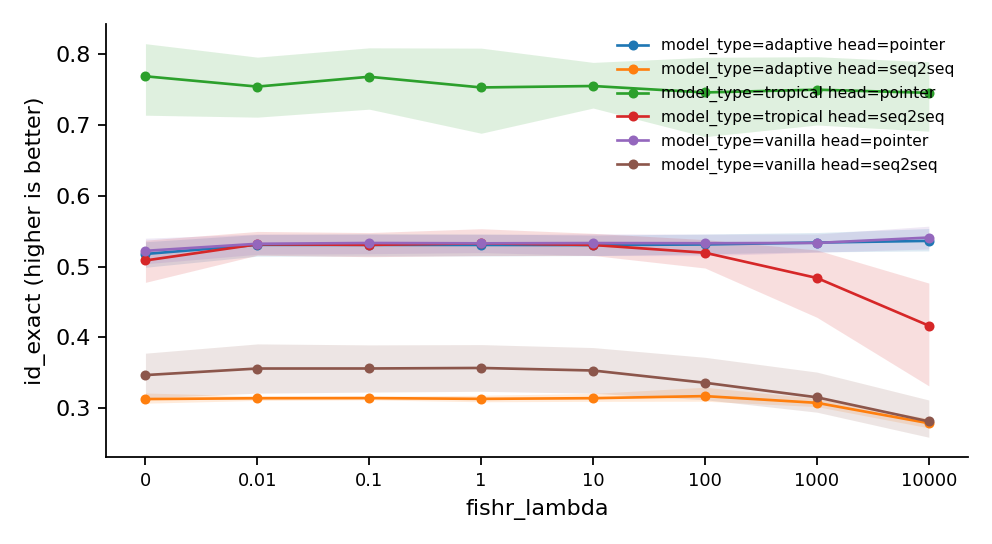
\includegraphics[width=\textwidth]{metric_id_exact.png}
\caption{\texttt{id\_exact} against \texttt{fishr\_lambda}: the mean over seeds with a 95\% bootstrap CI, one line per combination of the other factors.}
\label{fig:id_exact}
\end{figure}

{\small
\begin{longtable}{lllrlrrr}
\caption{\texttt{id\_exact} per cell: mean, 95\% bootstrap CI, SD, seeds, diverged runs.}\label{tab:summary-id_exact}\\
\toprule
\texttt{model\_type} & \texttt{head} & \texttt{fishr\_lambda} & mean & 95\% CI & SD & $n$ & div.\\
\midrule
\endhead
adaptive & pointer & 0 & 0.5179 & [0.499, 0.535] & 0.0237 & 5 & 0\\
adaptive & pointer & 0.01 & 0.5308 & [0.515, 0.545] & 0.0194 & 5 & 0\\
adaptive & pointer & 0.1 & 0.5307 & [0.515, 0.547] & 0.021 & 5 & 0\\
adaptive & pointer & 1 & 0.5307 & [0.515, 0.546] & 0.0216 & 5 & 0\\
adaptive & pointer & 10 & 0.5305 & [0.516, 0.545] & 0.0199 & 5 & 0\\
adaptive & pointer & 100 & 0.5313 & [0.518, 0.546] & 0.0188 & 5 & 0\\
adaptive & pointer & 1000 & 0.534 & [0.521, 0.548] & 0.0181 & 5 & 0\\
adaptive & pointer & 1e+04 & 0.5364 & [0.522, 0.554] & 0.0202 & 5 & 0\\
adaptive & seq2seq & 0 & 0.3131 & [0.307, 0.322] & 0.00972 & 5 & 0\\
adaptive & seq2seq & 0.01 & 0.3143 & [0.311, 0.318] & 0.00433 & 5 & 0\\
adaptive & seq2seq & 0.1 & 0.3145 & [0.312, 0.317] & 0.00341 & 5 & 0\\
adaptive & seq2seq & 1 & 0.3134 & [0.309, 0.318] & 0.00573 & 5 & 0\\
adaptive & seq2seq & 10 & 0.3143 & [0.31, 0.321] & 0.00762 & 5 & 0\\
adaptive & seq2seq & 100 & 0.3173 & [0.31, 0.33] & 0.0136 & 5 & 0\\
adaptive & seq2seq & 1000 & 0.3078 & [0.302, 0.314] & 0.00727 & 5 & 0\\
adaptive & seq2seq & 1e+04 & 0.279 & [0.272, 0.286] & 0.00851 & 5 & 0\\
tropical & pointer & 0 & 0.7687 & [0.714, 0.815] & 0.0663 & 5 & 0\\
tropical & pointer & 0.01 & 0.7542 & [0.711, 0.796] & 0.058 & 5 & 0\\
tropical & pointer & 0.1 & 0.7681 & [0.722, 0.809] & 0.0558 & 5 & 0\\
tropical & pointer & 1 & 0.753 & [0.688, 0.809] & 0.0808 & 5 & 0\\
tropical & pointer & 10 & 0.755 & [0.724, 0.788] & 0.0415 & 5 & 0\\
tropical & pointer & 100 & 0.7459 & [0.683, 0.796] & 0.0753 & 5 & 0\\
tropical & pointer & 1000 & 0.7498 & [0.7, 0.796] & 0.0625 & 5 & 0\\
tropical & pointer & 1e+04 & 0.7454 & [0.691, 0.789] & 0.0645 & 5 & 0\\
tropical & seq2seq & 0 & 0.5087 & [0.478, 0.537] & 0.0404 & 5 & 0\\
tropical & seq2seq & 0.01 & 0.5316 & [0.516, 0.55] & 0.0222 & 5 & 0\\
tropical & seq2seq & 0.1 & 0.5308 & [0.514, 0.548] & 0.0217 & 5 & 0\\
tropical & seq2seq & 1 & 0.5329 & [0.516, 0.554] & 0.0247 & 5 & 0\\
tropical & seq2seq & 10 & 0.5306 & [0.516, 0.547] & 0.0201 & 5 & 0\\
tropical & seq2seq & 100 & 0.5197 & [0.498, 0.538] & 0.0253 & 5 & 0\\
tropical & seq2seq & 1000 & 0.484 & [0.428, 0.523] & 0.0625 & 5 & 0\\
tropical & seq2seq & 1e+04 & 0.4167 & [0.332, 0.477] & 0.0953 & 5 & 0\\
vanilla & pointer & 0 & 0.5223 & [0.504, 0.54] & 0.022 & 5 & 0\\
vanilla & pointer & 0.01 & 0.5323 & [0.517, 0.546] & 0.0187 & 5 & 0\\
vanilla & pointer & 0.1 & 0.5334 & [0.518, 0.546] & 0.0171 & 5 & 0\\
vanilla & pointer & 1 & 0.5329 & [0.52, 0.545] & 0.0176 & 5 & 0\\
vanilla & pointer & 10 & 0.5333 & [0.516, 0.546] & 0.0185 & 5 & 0\\
vanilla & pointer & 100 & 0.5331 & [0.516, 0.546] & 0.0182 & 5 & 0\\
vanilla & pointer & 1000 & 0.5335 & [0.52, 0.546] & 0.0175 & 5 & 0\\
vanilla & pointer & 1e+04 & 0.5411 & [0.525, 0.557] & 0.0219 & 5 & 0\\
vanilla & seq2seq & 0 & 0.3469 & [0.315, 0.378] & 0.0393 & 5 & 0\\
vanilla & seq2seq & 0.01 & 0.3562 & [0.321, 0.391] & 0.0455 & 5 & 0\\
vanilla & seq2seq & 0.1 & 0.3563 & [0.323, 0.39] & 0.0446 & 5 & 0\\
vanilla & seq2seq & 1 & 0.357 & [0.324, 0.39] & 0.0425 & 5 & 0\\
vanilla & seq2seq & 10 & 0.3534 & [0.321, 0.386] & 0.0426 & 5 & 0\\
vanilla & seq2seq & 100 & 0.3361 & [0.312, 0.372] & 0.0396 & 5 & 0\\
vanilla & seq2seq & 1000 & 0.3156 & [0.295, 0.351] & 0.04 & 5 & 0\\
vanilla & seq2seq & 1e+04 & 0.2816 & [0.259, 0.312] & 0.0354 & 5 & 0\\
\bottomrule
\end{longtable}
}

{\small
\begin{longtable}{lllrrrl}
\caption{\texttt{id\_exact}: each level of \texttt{fishr\_lambda} against its control (0), within each combination of the other factors. parametric: Dunnett vs control.}\label{tab:control-id_exact}\\
\toprule
\texttt{model\_type} & \texttt{head} & \texttt{fishr\_lambda} & difference & 95\% CI & $p$ & \\
\midrule
\endhead
adaptive & pointer & 0.01 & 0.01286 & [-0.0228, 0.0485] & 0.8559 & \\
adaptive & pointer & 0.1 & 0.0128 & [-0.0228, 0.0484] & 0.8586 & \\
adaptive & pointer & 1 & 0.01274 & [-0.0229, 0.0484] & 0.8610 & \\
adaptive & pointer & 10 & 0.01256 & [-0.0231, 0.0482] & 0.8684 & \\
adaptive & pointer & 100 & 0.01342 & [-0.0222, 0.049] & 0.8312 & \\
adaptive & pointer & 1000 & 0.0161 & [-0.0195, 0.0517] & 0.6950 & \\
adaptive & pointer & 1e+04 & 0.01848 & [-0.0171, 0.0541] & 0.5645 & \\
adaptive & seq2seq & 0.01 & 0.00116 & [-0.013, 0.0153] & 1.0000 & \\
adaptive & seq2seq & 0.1 & 0.00136 & [-0.0128, 0.0155] & 0.9999 & \\
adaptive & seq2seq & 1 & $2.800\times10^{-4}$ & [-0.0139, 0.0145] & 1.0000 & \\
adaptive & seq2seq & 10 & 0.00124 & [-0.0129, 0.0154] & 1.0000 & \\
adaptive & seq2seq & 100 & 0.00416 & [-0.01, 0.0183] & 0.9397 & \\
adaptive & seq2seq & 1000 & -0.00534 & [-0.0195, 0.00883] & 0.8313 & \\
adaptive & seq2seq & 1e+04 & -0.0341 & [-0.0483, -0.0199] & $<10^{-4}$ & *\\
tropical & pointer & 0.01 & -0.01454 & [-0.126, 0.0974] & 0.9994 & \\
tropical & pointer & 0.1 & $-6.600\times10^{-4}$ & [-0.113, 0.111] & 1.0000 & \\
tropical & pointer & 1 & -0.01576 & [-0.128, 0.0962] & 0.9990 & \\
tropical & pointer & 10 & -0.01372 & [-0.126, 0.0982] & 0.9996 & \\
tropical & pointer & 100 & -0.02282 & [-0.135, 0.0891] & 0.9908 & \\
tropical & pointer & 1000 & -0.01892 & [-0.131, 0.093] & 0.9969 & \\
tropical & pointer & 1e+04 & -0.02336 & [-0.135, 0.0886] & 0.9895 & \\
tropical & seq2seq & 0.01 & 0.02288 & [-0.0582, 0.104] & 0.9498 & \\
tropical & seq2seq & 0.1 & 0.02204 & [-0.059, 0.103] & 0.9580 & \\
tropical & seq2seq & 1 & 0.02422 & [-0.0569, 0.105] & 0.9346 & \\
tropical & seq2seq & 10 & 0.0219 & [-0.0592, 0.103] & 0.9593 & \\
tropical & seq2seq & 100 & 0.01094 & [-0.0701, 0.092] & 0.9992 & \\
tropical & seq2seq & 1000 & -0.02468 & [-0.106, 0.0564] & 0.9289 & \\
tropical & seq2seq & 1e+04 & -0.09202 & [-0.173, -0.0109] & 0.0208 & *\\
vanilla & pointer & 0.01 & 0.00996 & [-0.0233, 0.0432] & 0.9337 & \\
vanilla & pointer & 0.1 & 0.01106 & [-0.0222, 0.0443] & 0.8958 & \\
vanilla & pointer & 1 & 0.0106 & [-0.0226, 0.0438] & 0.9128 & \\
vanilla & pointer & 10 & 0.01096 & [-0.0223, 0.0442] & 0.8996 & \\
vanilla & pointer & 100 & 0.01074 & [-0.0225, 0.044] & 0.9078 & \\
vanilla & pointer & 1000 & 0.01114 & [-0.0221, 0.0444] & 0.8926 & \\
vanilla & pointer & 1e+04 & 0.01878 & [-0.0145, 0.052] & 0.4776 & \\
vanilla & seq2seq & 0.01 & 0.00926 & [-0.0629, 0.0814] & 0.9994 & \\
vanilla & seq2seq & 0.1 & 0.00932 & [-0.0628, 0.0814] & 0.9994 & \\
vanilla & seq2seq & 1 & 0.01006 & [-0.0621, 0.0822] & 0.9991 & \\
vanilla & seq2seq & 10 & 0.00646 & [-0.0657, 0.0786] & 0.9999 & \\
vanilla & seq2seq & 100 & -0.01082 & [-0.0829, 0.0613] & 0.9985 & \\
vanilla & seq2seq & 1000 & -0.03136 & [-0.103, 0.0408] & 0.7281 & \\
vanilla & seq2seq & 1e+04 & -0.06534 & [-0.137, 0.00678] & 0.0887 & \\
\bottomrule
\end{longtable}
}

{\small
\begin{longtable}{llrrrrr}
\caption{\texttt{id\_exact} against log10 \texttt{fishr\_lambda}: parametric: OLS slope t-test, seed-bootstrap CI, with the Jonckheere--Terpstra ordered-trend $\tau$ and $p$.}\label{tab:trend-id_exact}\\
\toprule
\texttt{model\_type} & \texttt{head} & estimate & 95\% CI & $p$ & JT $\tau$ & JT $p$\\
\midrule
\endhead
adaptive & pointer & $8.621\times10^{-4}$ & [$2.71\times10^{-5}$, 0.00161] & 0.5821 & 0.0495 & 0.7237\\
adaptive & seq2seq & -0.004118 & [-0.00508, -0.00328] & 0.0003 & -0.491 & 0.0002\\
tropical & pointer & -0.002501 & [-0.00487, $-1.34\times10^{-4}$] & 0.6191 & -0.0438 & 0.7580\\
tropical & seq2seq & -0.01612 & [-0.0271, -0.0082] & 0.0006 & -0.45 & 0.0012\\
vanilla & pointer & $9.557\times10^{-4}$ & [$5.24\times10^{-4}$, 0.00138] & 0.5164 & 0.137 & 0.3109\\
vanilla & seq2seq & -0.01164 & [-0.0182, -0.00509] & 0.0018 & -0.413 & 0.0028\\
\bottomrule
\end{longtable}
}

{\small
\begin{longtable}{lrrrl}
\caption{\texttt{id\_exact}: paired contrasts by seed, Holm-corrected across the cells. parametric: paired t-test by seed, Holm.}\label{tab:paired-id_exact}\\
\toprule
contrast (within) & difference & 95\% CI & $p$ & \\
\midrule
\endhead
\stackcell{model\_type: tropical - vanilla\\\footnotesize head=pointer fishr\_lambda=0 } & 0.2464 & [0.168, 0.324] & 0.0094 & *\\
\stackcell{model\_type: tropical - vanilla\\\footnotesize head=pointer fishr\_lambda=0.01 } & 0.2219 & [0.157, 0.287] & 0.0094 & *\\
\stackcell{model\_type: tropical - vanilla\\\footnotesize head=pointer fishr\_lambda=0.1 } & 0.2347 & [0.176, 0.294] & 0.0057 & *\\
\stackcell{model\_type: tropical - vanilla\\\footnotesize head=pointer fishr\_lambda=1 } & 0.22 & [0.134, 0.306] & 0.0133 & *\\
\stackcell{model\_type: tropical - vanilla\\\footnotesize head=pointer fishr\_lambda=10 } & 0.2217 & [0.178, 0.265] & 0.0024 & *\\
\stackcell{model\_type: tropical - vanilla\\\footnotesize head=pointer fishr\_lambda=100 } & 0.2128 & [0.134, 0.291] & 0.0133 & *\\
\stackcell{model\_type: tropical - vanilla\\\footnotesize head=pointer fishr\_lambda=1000 } & 0.2163 & [0.152, 0.281] & 0.0094 & *\\
\stackcell{model\_type: tropical - vanilla\\\footnotesize head=pointer fishr\_lambda=1e+04 } & 0.2043 & [0.145, 0.264] & 0.0094 & *\\
\stackcell{model\_type: tropical - vanilla\\\footnotesize head=seq2seq fishr\_lambda=0 } & 0.1618 & [0.1, 0.223] & 0.0133 & *\\
\stackcell{model\_type: tropical - vanilla\\\footnotesize head=seq2seq fishr\_lambda=0.01 } & 0.1754 & [0.104, 0.247] & 0.0133 & *\\
\stackcell{model\_type: tropical - vanilla\\\footnotesize head=seq2seq fishr\_lambda=0.1 } & 0.1745 & [0.109, 0.24] & 0.0133 & *\\
\stackcell{model\_type: tropical - vanilla\\\footnotesize head=seq2seq fishr\_lambda=1 } & 0.1759 & [0.111, 0.241] & 0.0133 & *\\
\stackcell{model\_type: tropical - vanilla\\\footnotesize head=seq2seq fishr\_lambda=10 } & 0.1772 & [0.116, 0.238] & 0.0115 & *\\
\stackcell{model\_type: tropical - vanilla\\\footnotesize head=seq2seq fishr\_lambda=100 } & 0.1835 & [0.127, 0.24] & 0.0094 & *\\
\stackcell{model\_type: tropical - vanilla\\\footnotesize head=seq2seq fishr\_lambda=1000 } & 0.1685 & [0.0826, 0.254] & 0.0133 & *\\
\stackcell{model\_type: tropical - vanilla\\\footnotesize head=seq2seq fishr\_lambda=1e+04 } & 0.1351 & [0.0225, 0.248] & 0.0291 & *\\
\stackcell{model\_type: adaptive - vanilla\\\footnotesize head=pointer fishr\_lambda=0 } & -0.00442 & [-0.0262, 0.0174] & 1.0000 & \\
\stackcell{model\_type: adaptive - vanilla\\\footnotesize head=pointer fishr\_lambda=0.01 } & -0.00152 & [-0.0152, 0.0122] & 1.0000 & \\
\stackcell{model\_type: adaptive - vanilla\\\footnotesize head=pointer fishr\_lambda=0.1 } & -0.00268 & [-0.0168, 0.0115] & 1.0000 & \\
\stackcell{model\_type: adaptive - vanilla\\\footnotesize head=pointer fishr\_lambda=1 } & -0.00228 & [-0.0155, 0.0109] & 1.0000 & \\
\stackcell{model\_type: adaptive - vanilla\\\footnotesize head=pointer fishr\_lambda=10 } & -0.00282 & [-0.0131, 0.00742] & 1.0000 & \\
\stackcell{model\_type: adaptive - vanilla\\\footnotesize head=pointer fishr\_lambda=100 } & -0.00174 & [-0.0136, 0.0102] & 1.0000 & \\
\stackcell{model\_type: adaptive - vanilla\\\footnotesize head=pointer fishr\_lambda=1000 } & $5.400\times10^{-4}$ & [-0.012, 0.0131] & 1.0000 & \\
\stackcell{model\_type: adaptive - vanilla\\\footnotesize head=pointer fishr\_lambda=1e+04 } & -0.00472 & [-0.0226, 0.0132] & 1.0000 & \\
\stackcell{model\_type: adaptive - vanilla\\\footnotesize head=seq2seq fishr\_lambda=0 } & -0.03384 & [-0.0885, 0.0208] & 1.0000 & \\
\stackcell{model\_type: adaptive - vanilla\\\footnotesize head=seq2seq fishr\_lambda=0.01 } & -0.04194 & [-0.0998, 0.016] & 1.0000 & \\
\stackcell{model\_type: adaptive - vanilla\\\footnotesize head=seq2seq fishr\_lambda=0.1 } & -0.0418 & [-0.0979, 0.0143] & 1.0000 & \\
\stackcell{model\_type: adaptive - vanilla\\\footnotesize head=seq2seq fishr\_lambda=1 } & -0.04362 & [-0.0977, 0.0105] & 1.0000 & \\
\stackcell{model\_type: adaptive - vanilla\\\footnotesize head=seq2seq fishr\_lambda=10 } & -0.03906 & [-0.0941, 0.016] & 1.0000 & \\
\stackcell{model\_type: adaptive - vanilla\\\footnotesize head=seq2seq fishr\_lambda=100 } & -0.01886 & [-0.0764, 0.0387] & 1.0000 & \\
\stackcell{model\_type: adaptive - vanilla\\\footnotesize head=seq2seq fishr\_lambda=1000 } & -0.00782 & [-0.0602, 0.0446] & 1.0000 & \\
\stackcell{model\_type: adaptive - vanilla\\\footnotesize head=seq2seq fishr\_lambda=1e+04 } & -0.0026 & [-0.0491, 0.0439] & 1.0000 & \\
\stackcell{head: pointer - seq2seq\\\footnotesize model\_type=adaptive fishr\_lambda=0 } & 0.2048 & [0.177, 0.232] & 0.0005 & *\\
\stackcell{head: pointer - seq2seq\\\footnotesize model\_type=adaptive fishr\_lambda=0.01 } & 0.2165 & [0.192, 0.241] & 0.0003 & *\\
\stackcell{head: pointer - seq2seq\\\footnotesize model\_type=adaptive fishr\_lambda=0.1 } & 0.2163 & [0.19, 0.242] & 0.0004 & *\\
\stackcell{head: pointer - seq2seq\\\footnotesize model\_type=adaptive fishr\_lambda=1 } & 0.2173 & [0.194, 0.241] & 0.0003 & *\\
\stackcell{head: pointer - seq2seq\\\footnotesize model\_type=adaptive fishr\_lambda=10 } & 0.2161 & [0.192, 0.24] & 0.0003 & *\\
\stackcell{head: pointer - seq2seq\\\footnotesize model\_type=adaptive fishr\_lambda=100 } & 0.2141 & [0.188, 0.24] & 0.0004 & *\\
\stackcell{head: pointer - seq2seq\\\footnotesize model\_type=adaptive fishr\_lambda=1000 } & 0.2263 & [0.2, 0.253] & 0.0004 & *\\
\stackcell{head: pointer - seq2seq\\\footnotesize model\_type=adaptive fishr\_lambda=1e+04 } & 0.2574 & [0.236, 0.279] & 0.0001 & *\\
\stackcell{head: pointer - seq2seq\\\footnotesize model\_type=tropical fishr\_lambda=0 } & 0.26 & [0.177, 0.343] & 0.0104 & *\\
\stackcell{head: pointer - seq2seq\\\footnotesize model\_type=tropical fishr\_lambda=0.01 } & 0.2226 & [0.164, 0.281] & 0.0060 & *\\
\stackcell{head: pointer - seq2seq\\\footnotesize model\_type=tropical fishr\_lambda=0.1 } & 0.2373 & [0.181, 0.293] & 0.0045 & *\\
\stackcell{head: pointer - seq2seq\\\footnotesize model\_type=tropical fishr\_lambda=1 } & 0.22 & [0.128, 0.312] & 0.0122 & *\\
\stackcell{head: pointer - seq2seq\\\footnotesize model\_type=tropical fishr\_lambda=10 } & 0.2244 & [0.178, 0.27] & 0.0028 & *\\
\stackcell{head: pointer - seq2seq\\\footnotesize model\_type=tropical fishr\_lambda=100 } & 0.2263 & [0.137, 0.315] & 0.0122 & *\\
\stackcell{head: pointer - seq2seq\\\footnotesize model\_type=tropical fishr\_lambda=1000 } & 0.2658 & [0.182, 0.35] & 0.0104 & *\\
\stackcell{head: pointer - seq2seq\\\footnotesize model\_type=tropical fishr\_lambda=1e+04 } & 0.3287 & [0.188, 0.47] & 0.0122 & *\\
\stackcell{head: pointer - seq2seq\\\footnotesize model\_type=vanilla fishr\_lambda=0 } & 0.1754 & [0.12, 0.231] & 0.0104 & *\\
\stackcell{head: pointer - seq2seq\\\footnotesize model\_type=vanilla fishr\_lambda=0.01 } & 0.1761 & [0.105, 0.247] & 0.0122 & *\\
\stackcell{head: pointer - seq2seq\\\footnotesize model\_type=vanilla fishr\_lambda=0.1 } & 0.1771 & [0.107, 0.247] & 0.0122 & *\\
\stackcell{head: pointer - seq2seq\\\footnotesize model\_type=vanilla fishr\_lambda=1 } & 0.1759 & [0.11, 0.242] & 0.0122 & *\\
\stackcell{head: pointer - seq2seq\\\footnotesize model\_type=vanilla fishr\_lambda=10 } & 0.1799 & [0.113, 0.247] & 0.0122 & *\\
\stackcell{head: pointer - seq2seq\\\footnotesize model\_type=vanilla fishr\_lambda=100 } & 0.197 & [0.13, 0.264] & 0.0104 & *\\
\stackcell{head: pointer - seq2seq\\\footnotesize model\_type=vanilla fishr\_lambda=1000 } & 0.2179 & [0.15, 0.286] & 0.0104 & *\\
\stackcell{head: pointer - seq2seq\\\footnotesize model\_type=vanilla fishr\_lambda=1e+04 } & 0.2595 & [0.192, 0.327] & 0.0060 & *\\
\bottomrule
\end{longtable}
}


\section{Curves}
\begin{figure}[tbp]
\centering
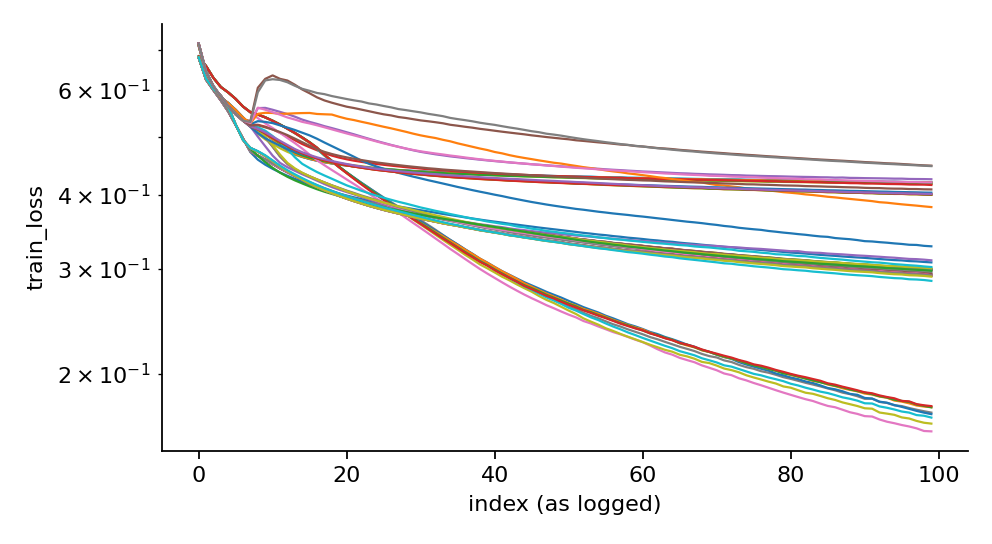
\includegraphics[width=\textwidth]{curve_train_loss.png}
\caption{\texttt{train\_loss}, the mean over seeds per cell.}
\label{fig:curve-1}
\end{figure}
\begin{figure}[tbp]
\centering
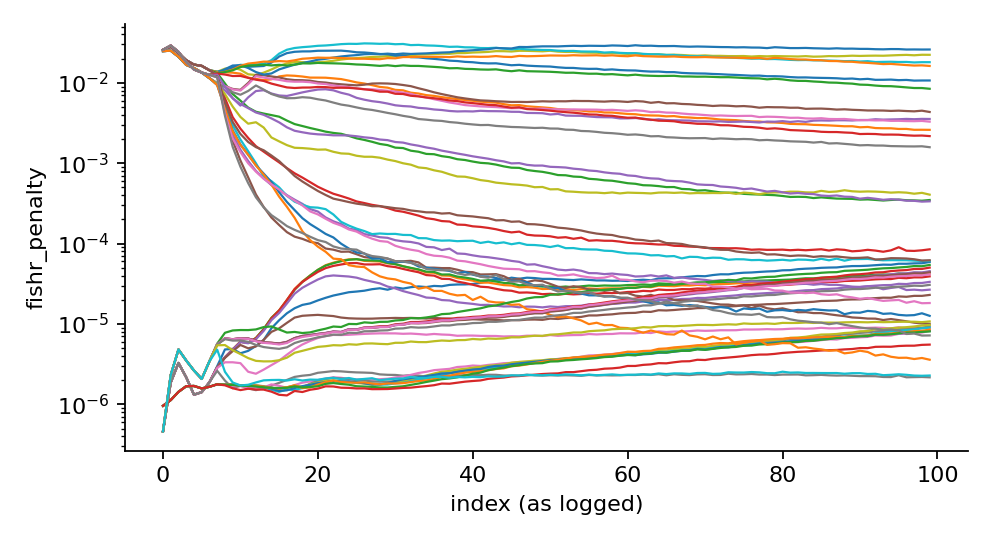
\includegraphics[width=\textwidth]{curve_fishr_penalty.png}
\caption{\texttt{fishr\_penalty}, the mean over seeds per cell.}
\label{fig:curve-2}
\end{figure}
\begin{figure}[tbp]
\centering
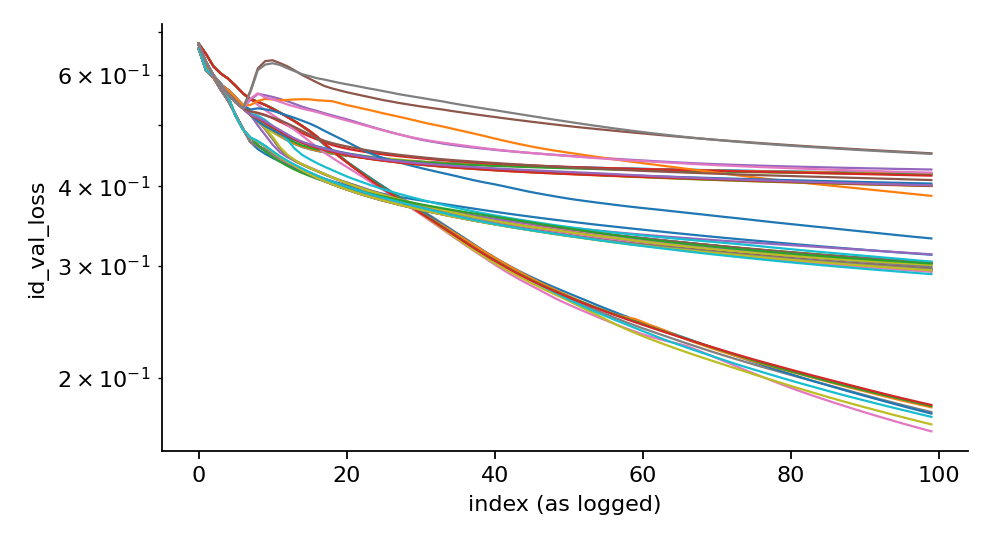
\includegraphics[width=\textwidth]{curve_id_val_loss.png}
\caption{\texttt{id\_val\_loss}, the mean over seeds per cell.}
\label{fig:curve-3}
\end{figure}

\section{Configuration}
The base configuration every run shares (frozen hash \texttt{69813b292d06}); factor levels are in \autoref{tab:summary-ood_len_f1}.
{\footnotesize
\begin{verbatim}
task:
  name: LISDataset
  value_range:
  - 1
  - 10
  target_range: null
  weight_range: null
  adversarial_range:
  - 10
  - 30
  noise_prob: 0.0
data:
  train_lengths:
  - 4
  - 5
  - 6
  - 7
  - 8
  ood_lengths:
  - 12
  - 16
  - 64
  ood_value_range: null
  ood_noise_range: null
  ood_noise_prob: 0.5
  n_per_length: 20000
  n_eval_per_length: 2000
  curve_eval_limit: 256
model:
  d_model: 64
  n_heads: 2
  num_layers: 1
  dropout: 0.0
  tropical_impl: legacy
optim:
  lr: 0.0001
  epochs: 100
  batch_size: 100
  eval_batch_size: 256
fishr:
  ema: 0.95
  anneal_iters: 1500
  reset_optimizer: true
\end{verbatim}
}
Store: \texttt{campaigns/tropical/LIS/results}.
\end{document}